\documentclass[../Bachelorarbeit.tex]{subfiles}

\begin{document}
\captionsetup[figure]{list=no}
\begin{figure}
    \centering
    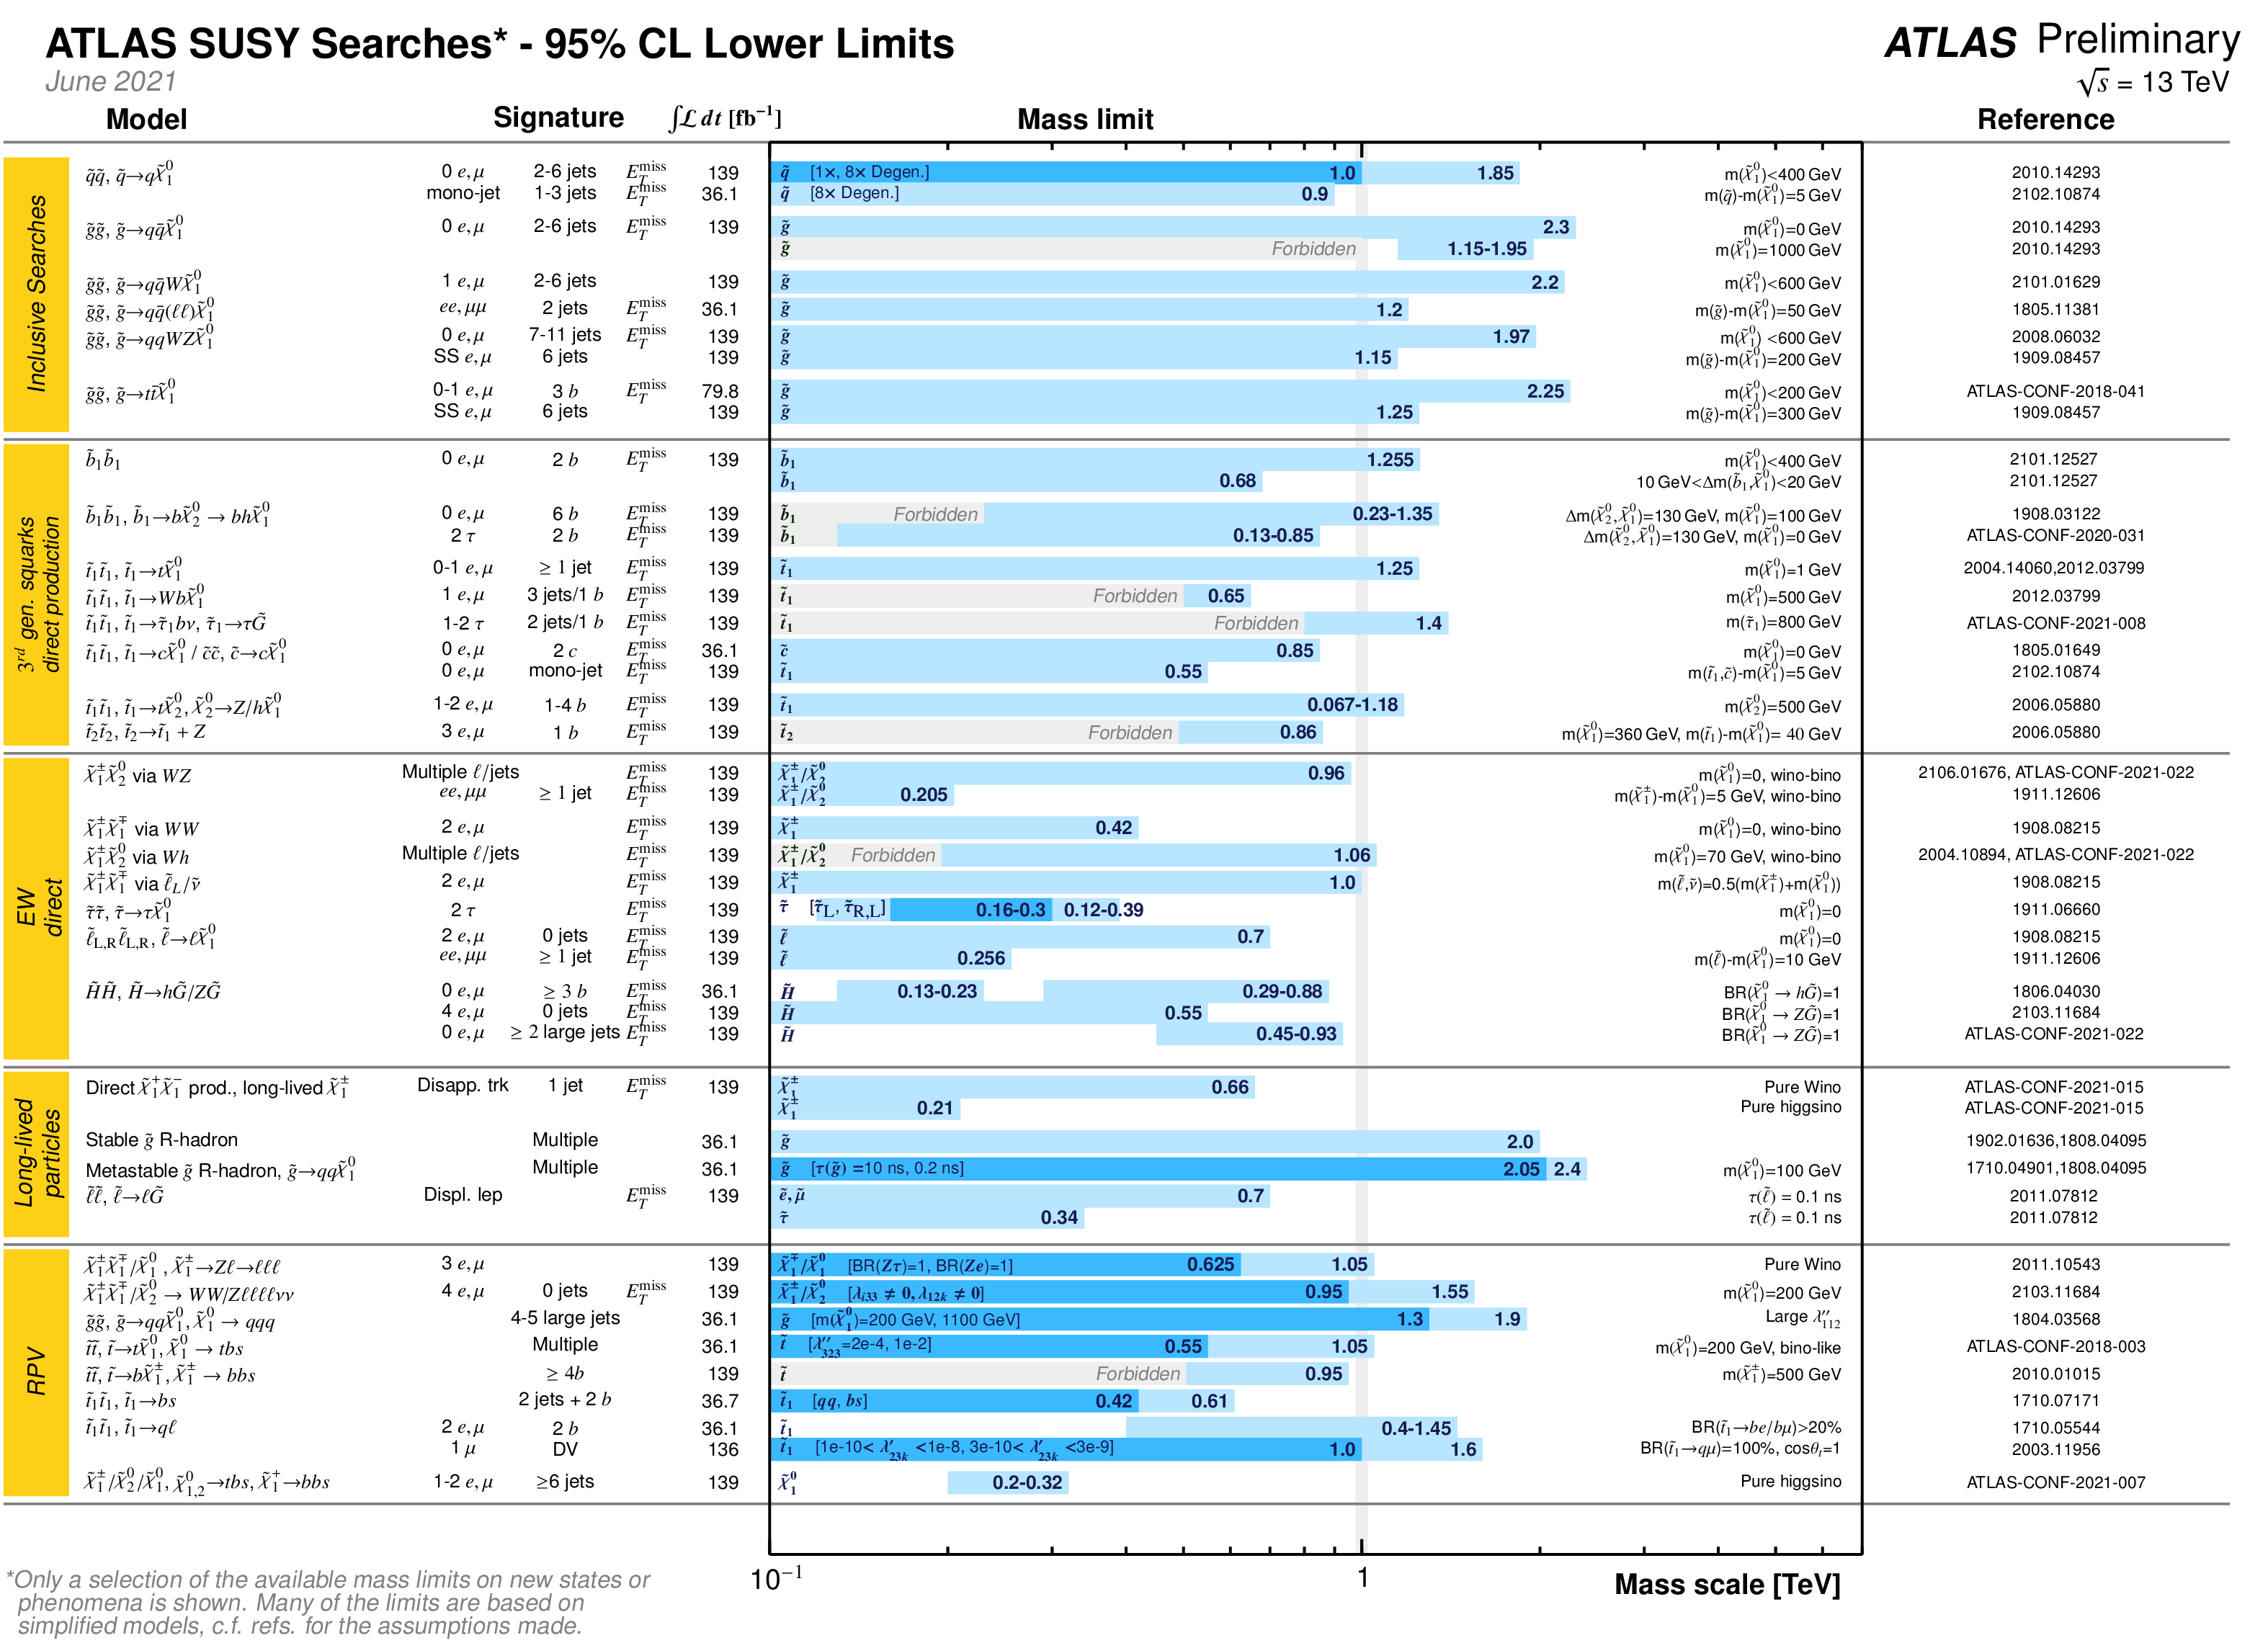
\includegraphics[width=\textwidth]{images/fig_23_ATLAS_SUSY.png}
    \caption{Example for SUSY as \acrshort{bsm} Model. All particles shown here have been rejected as they should have been found using described methods in \acrshort{bsm} search.  \cite{.07.06.2021}}
    \label{fig:ATLAS_SUSY}
\end{figure}

\section{Significance of dim-8 operators}
\label{sec:signif_dim8}


\begin{figure}[h]
    \centering
    \begin{subfigure}{0.45\textwidth}
        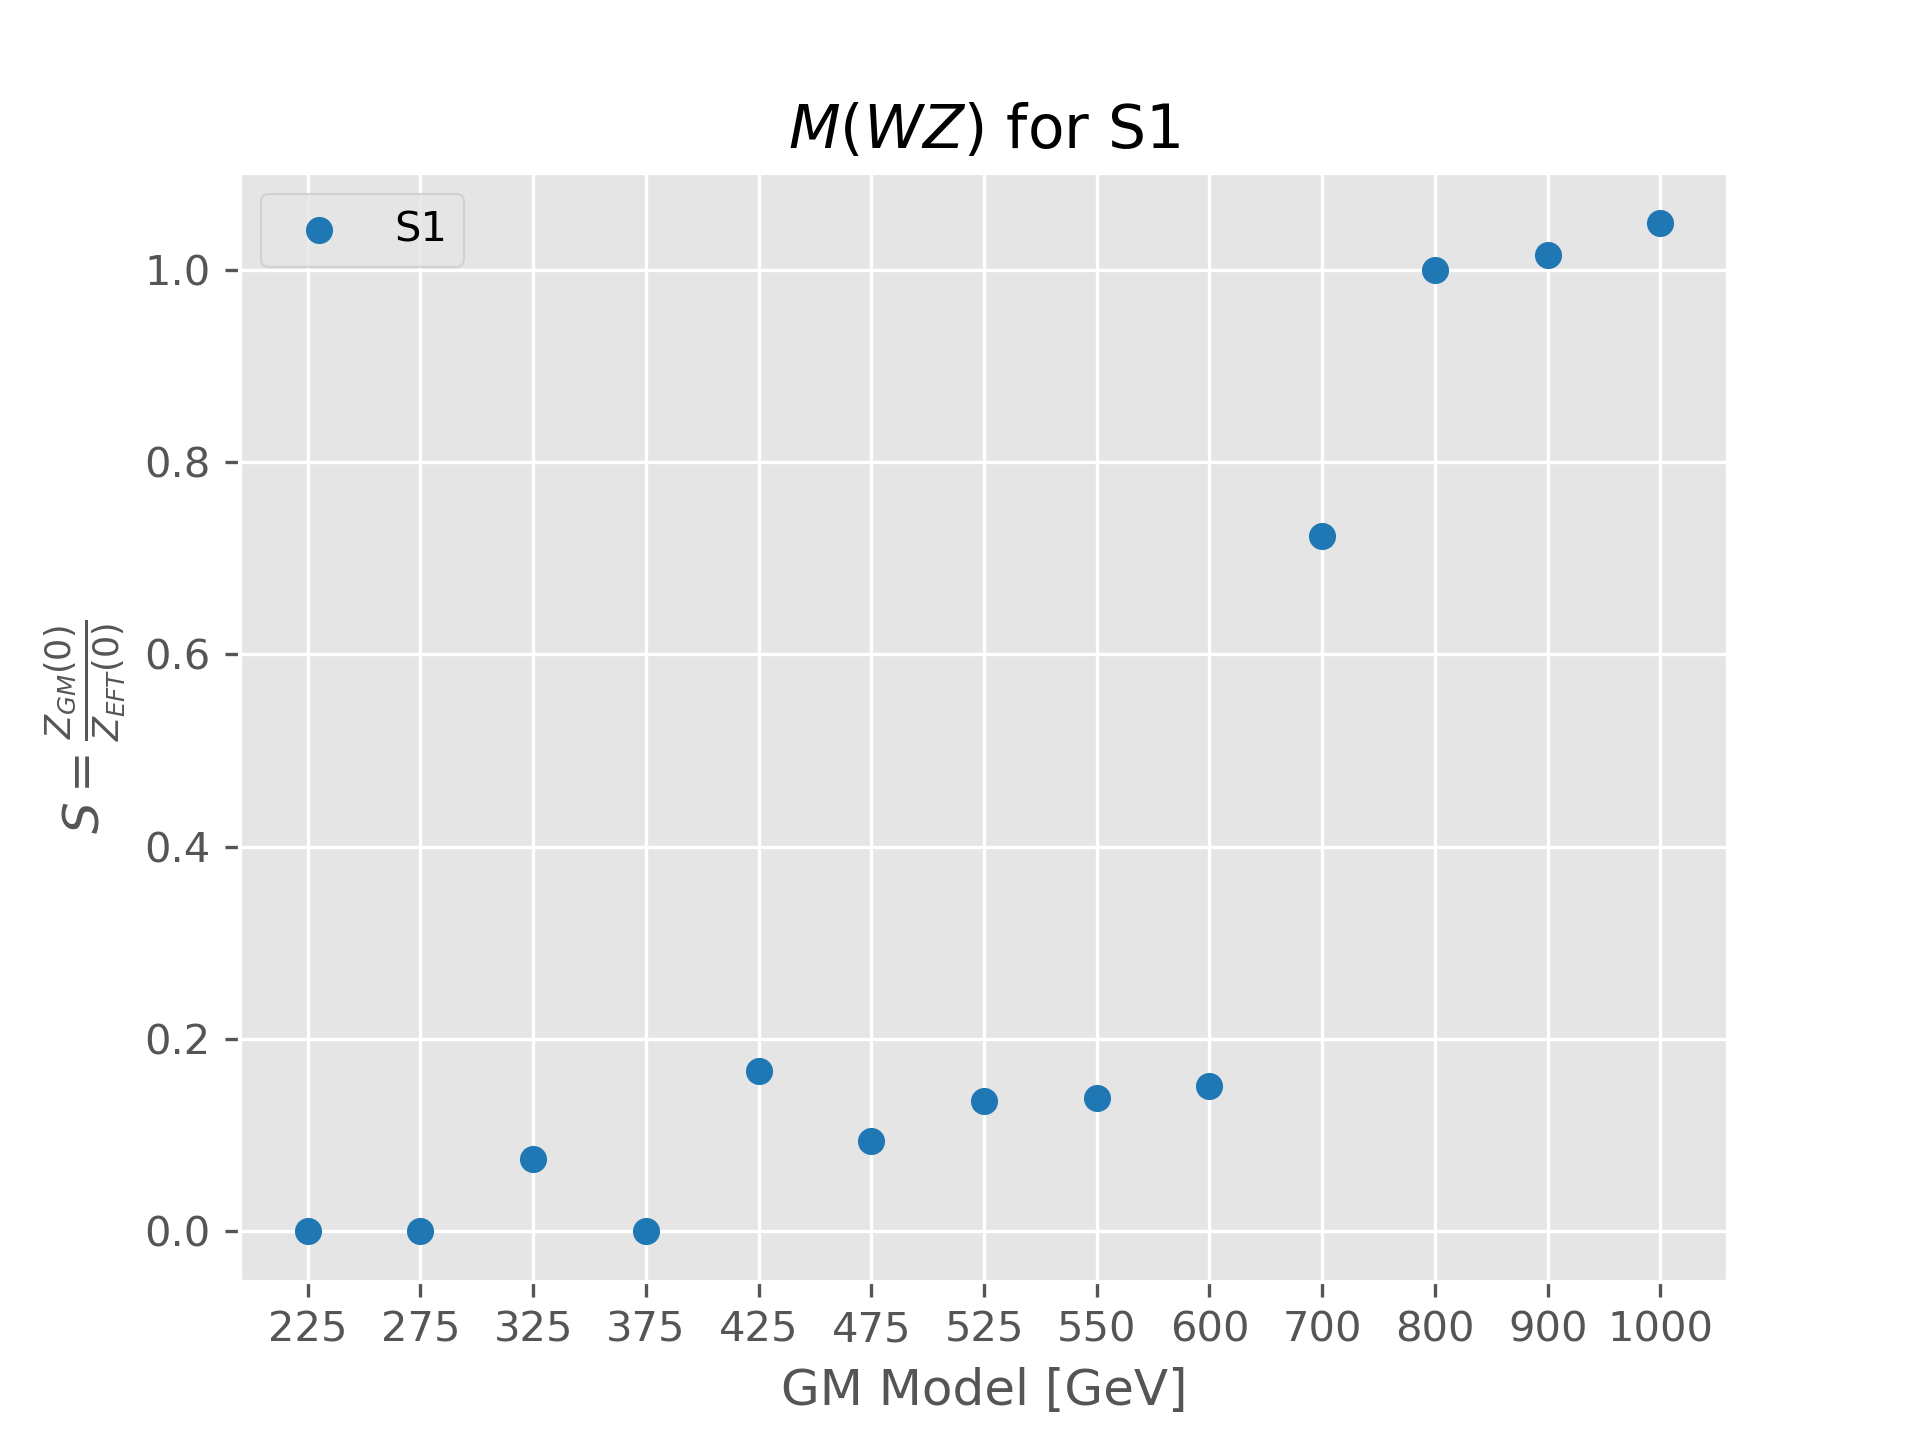
\includegraphics[width=\textwidth]{Plots/gm_relevanze/MWZ_op_S1.png}

    \end{subfigure}
    \begin{subfigure}{0.45\textwidth}
        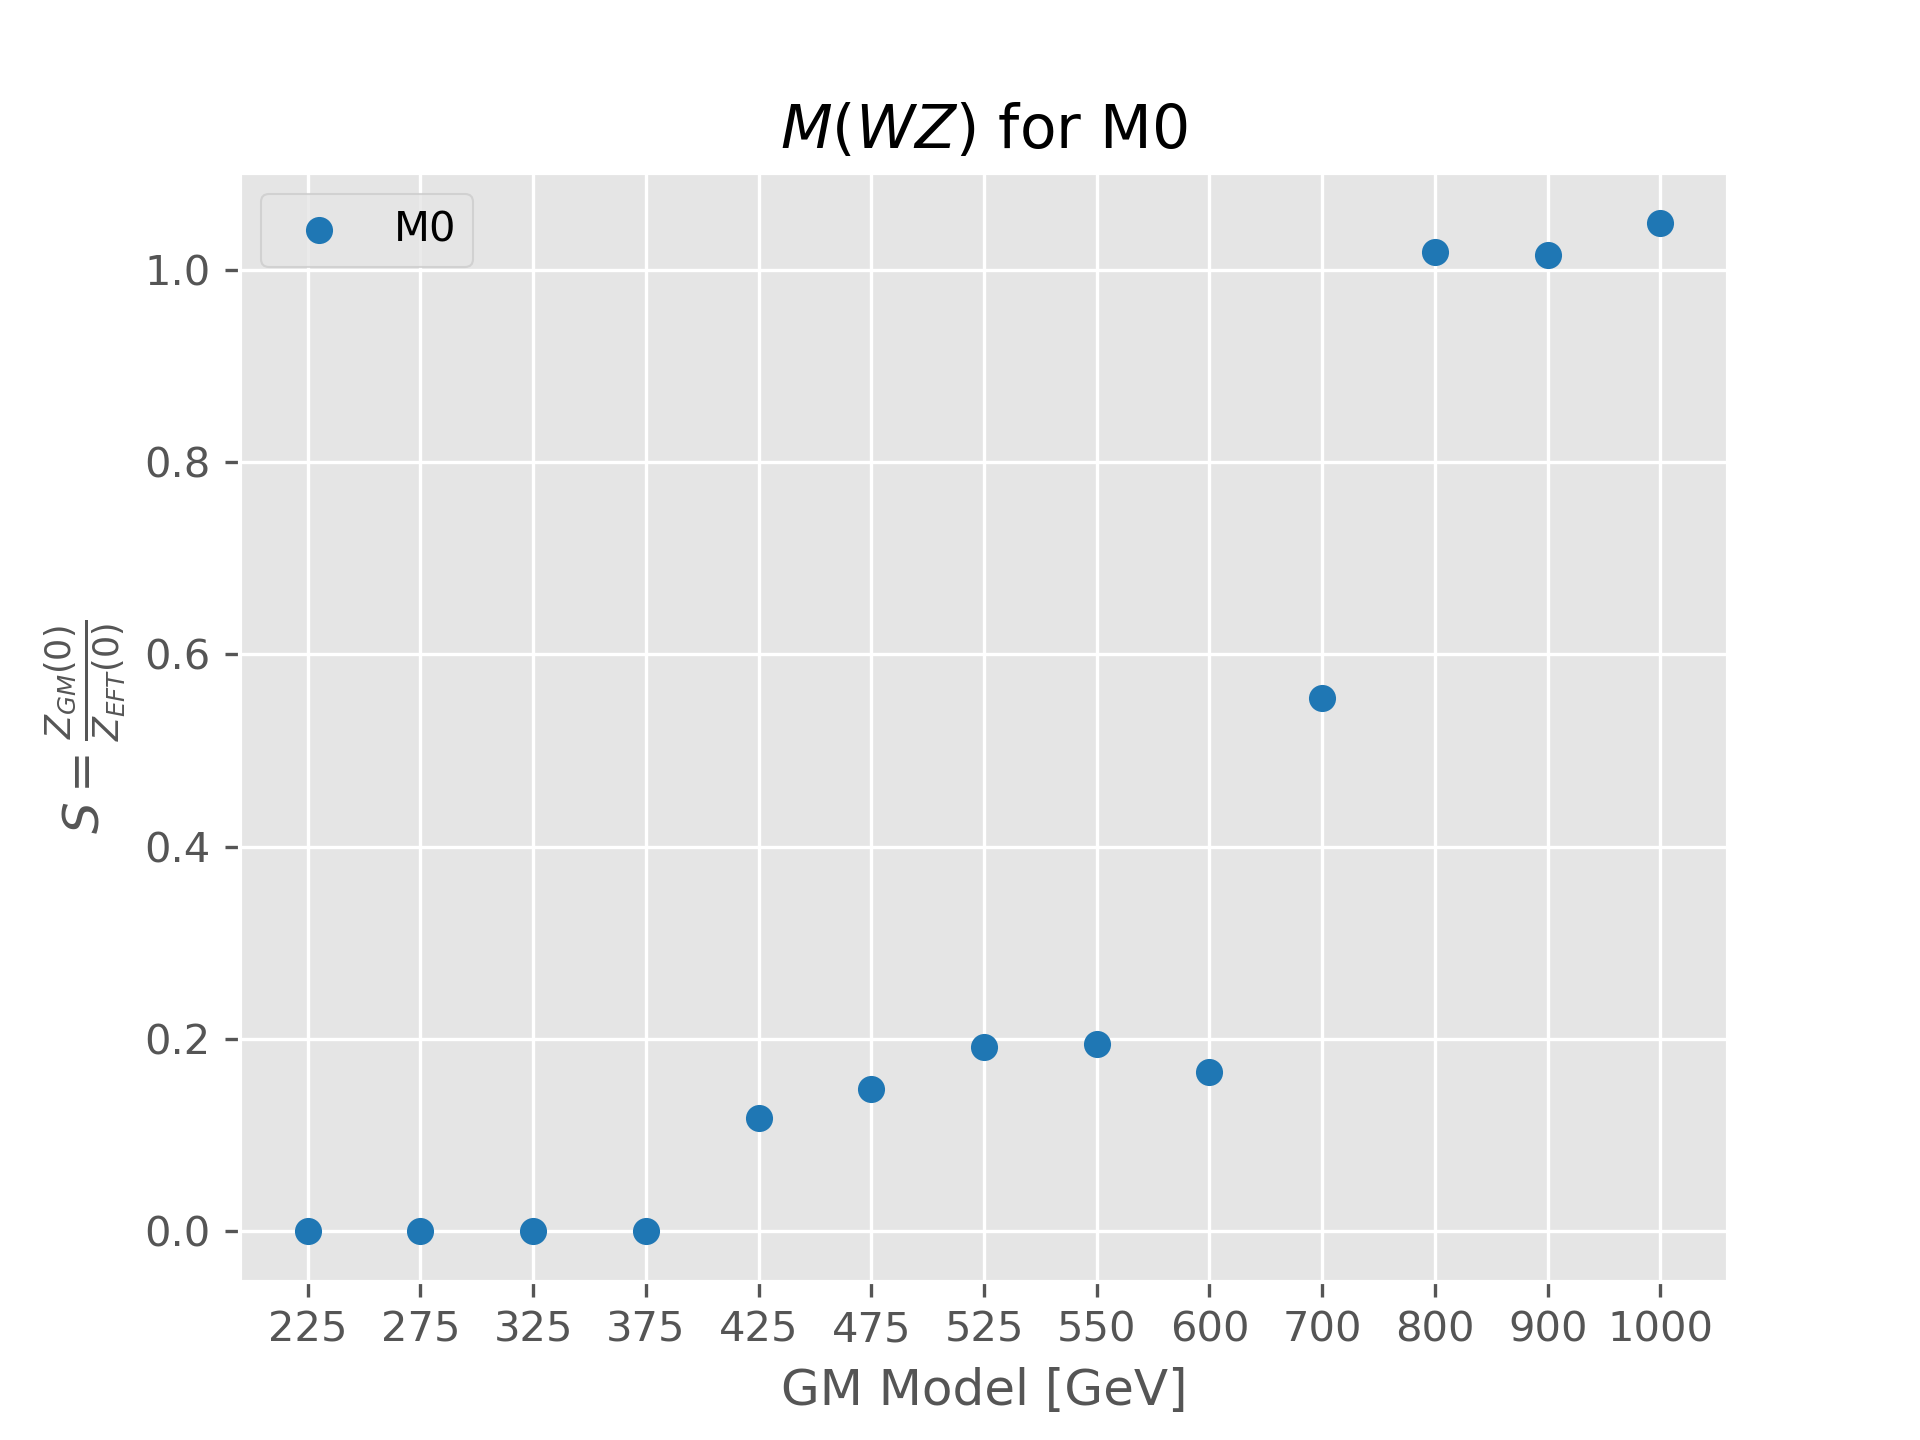
\includegraphics[width=\textwidth]{Plots/gm_relevanze/MWZ_op_M0.png}

    \end{subfigure}
    \begin{subfigure}{0.45\textwidth}
        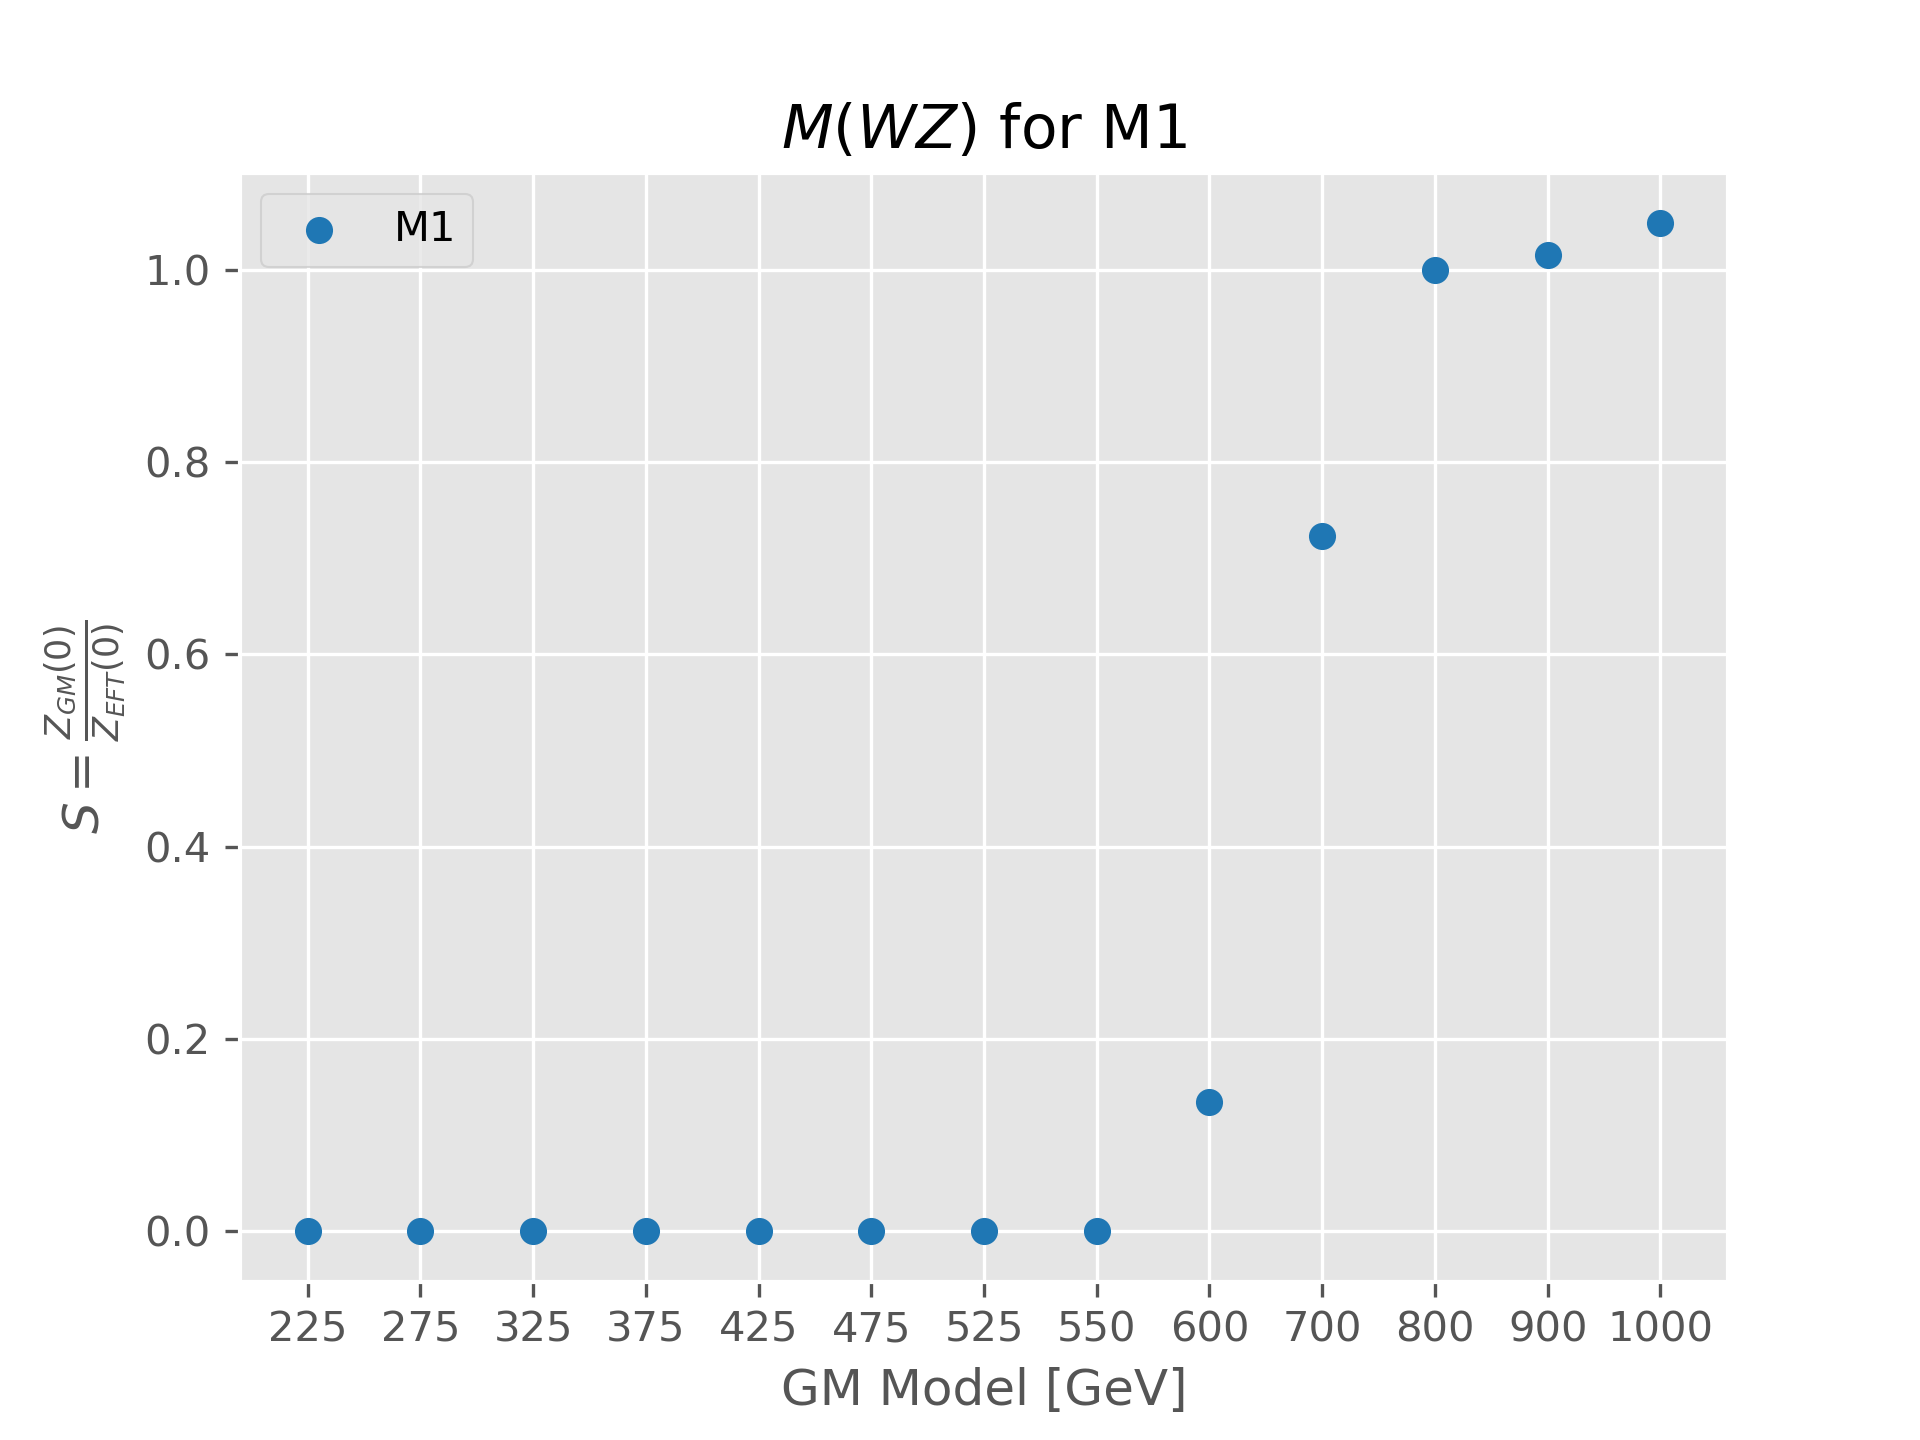
\includegraphics[width=\textwidth]{Plots/gm_relevanze/MWZ_op_M1.png}

    \end{subfigure}
    \begin{subfigure}{0.45\textwidth}
        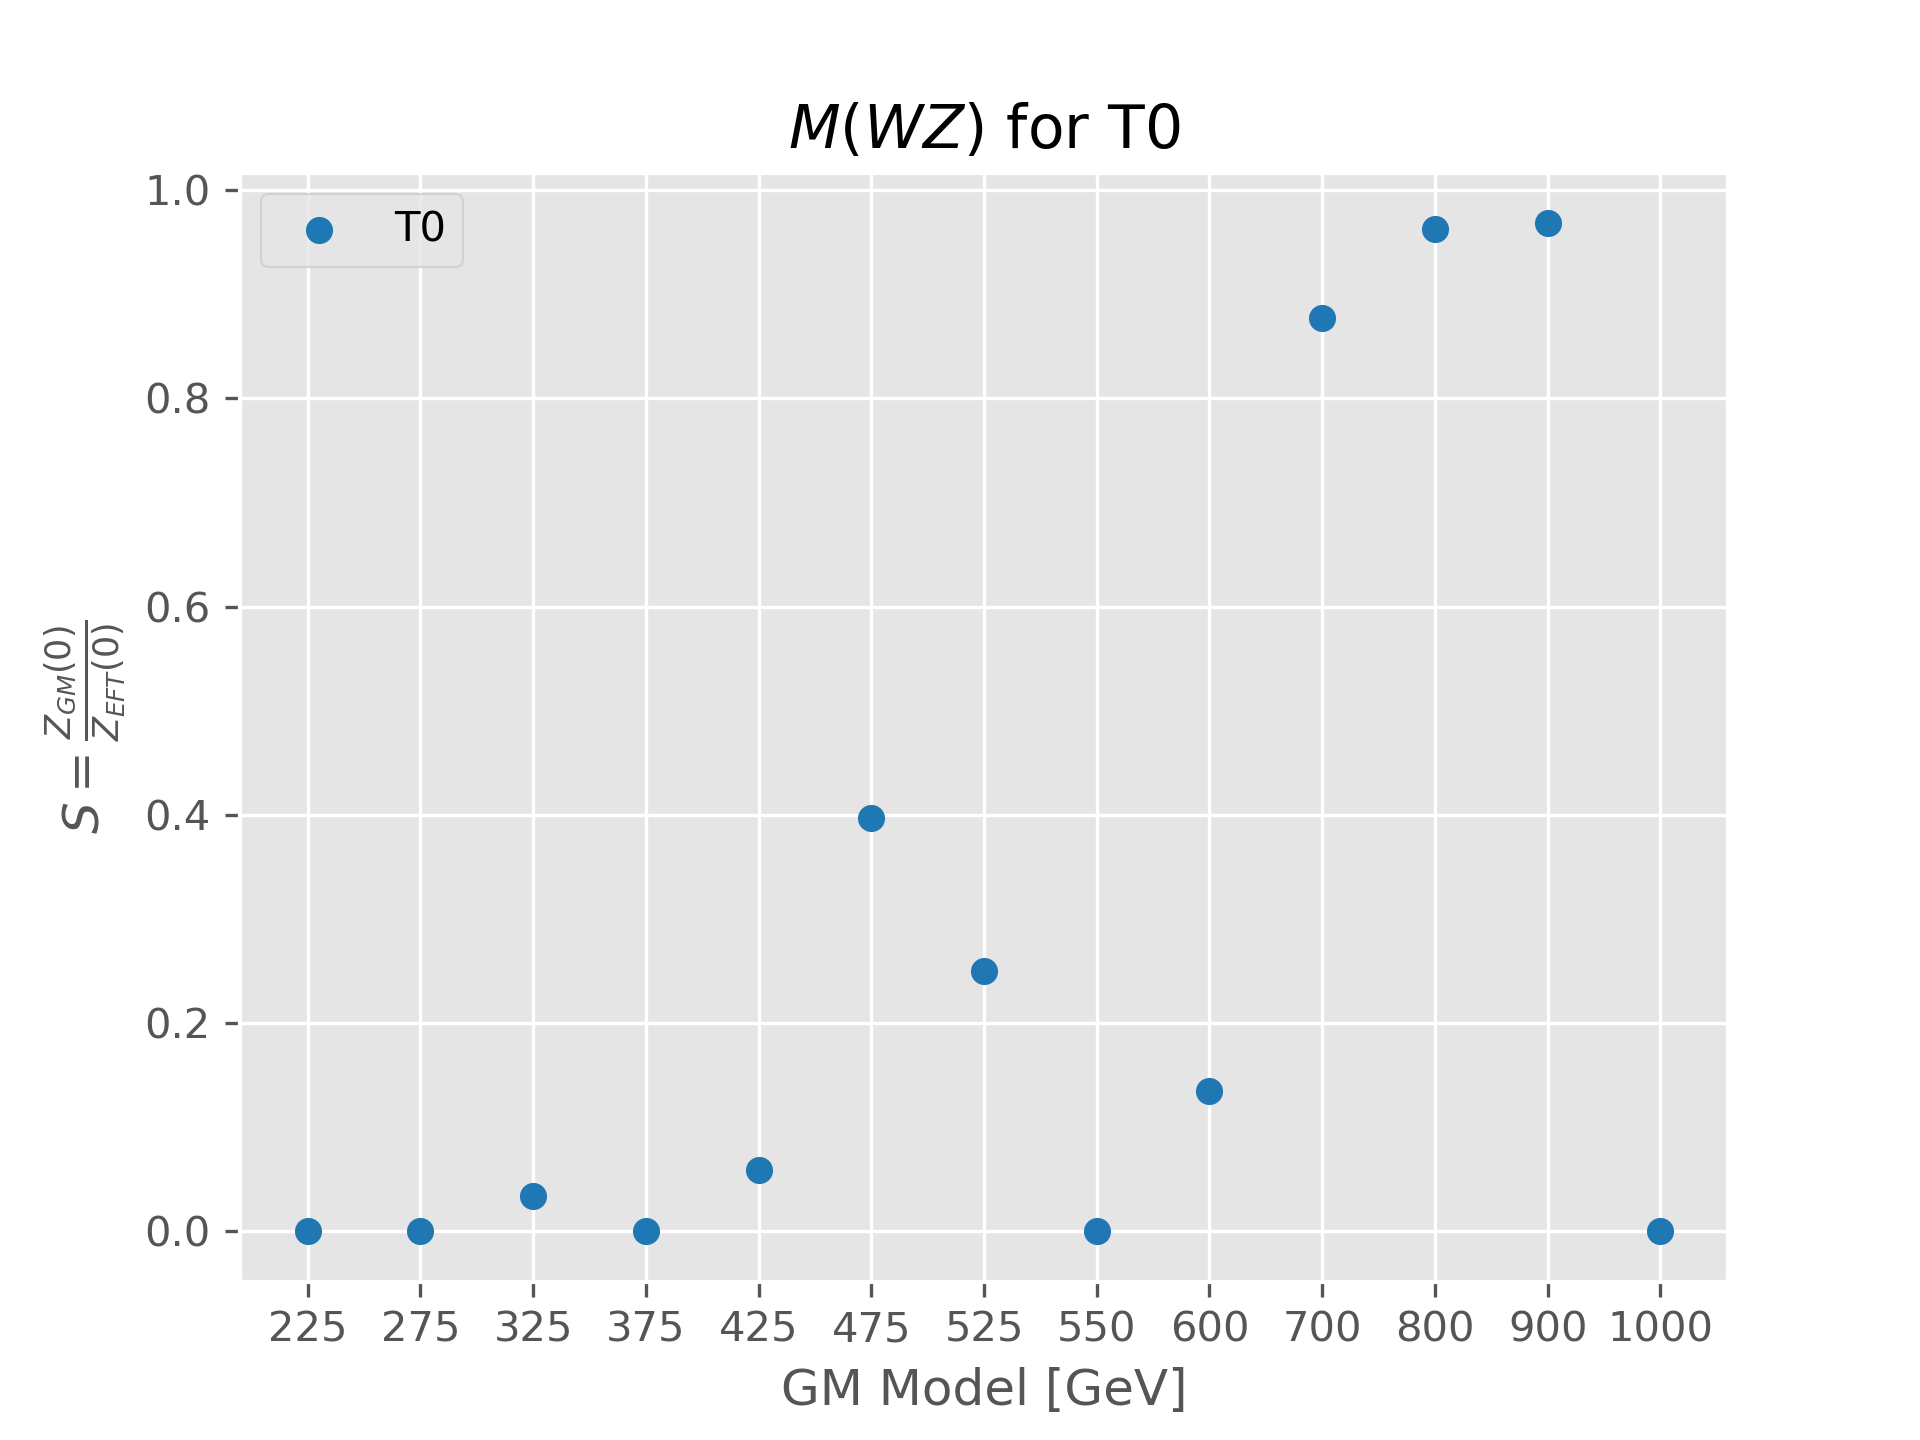
\includegraphics[width=\textwidth]{Plots/gm_relevanze/MWZ_op_T0.png}

    \end{subfigure}
    \begin{subfigure}{0.45\textwidth}
        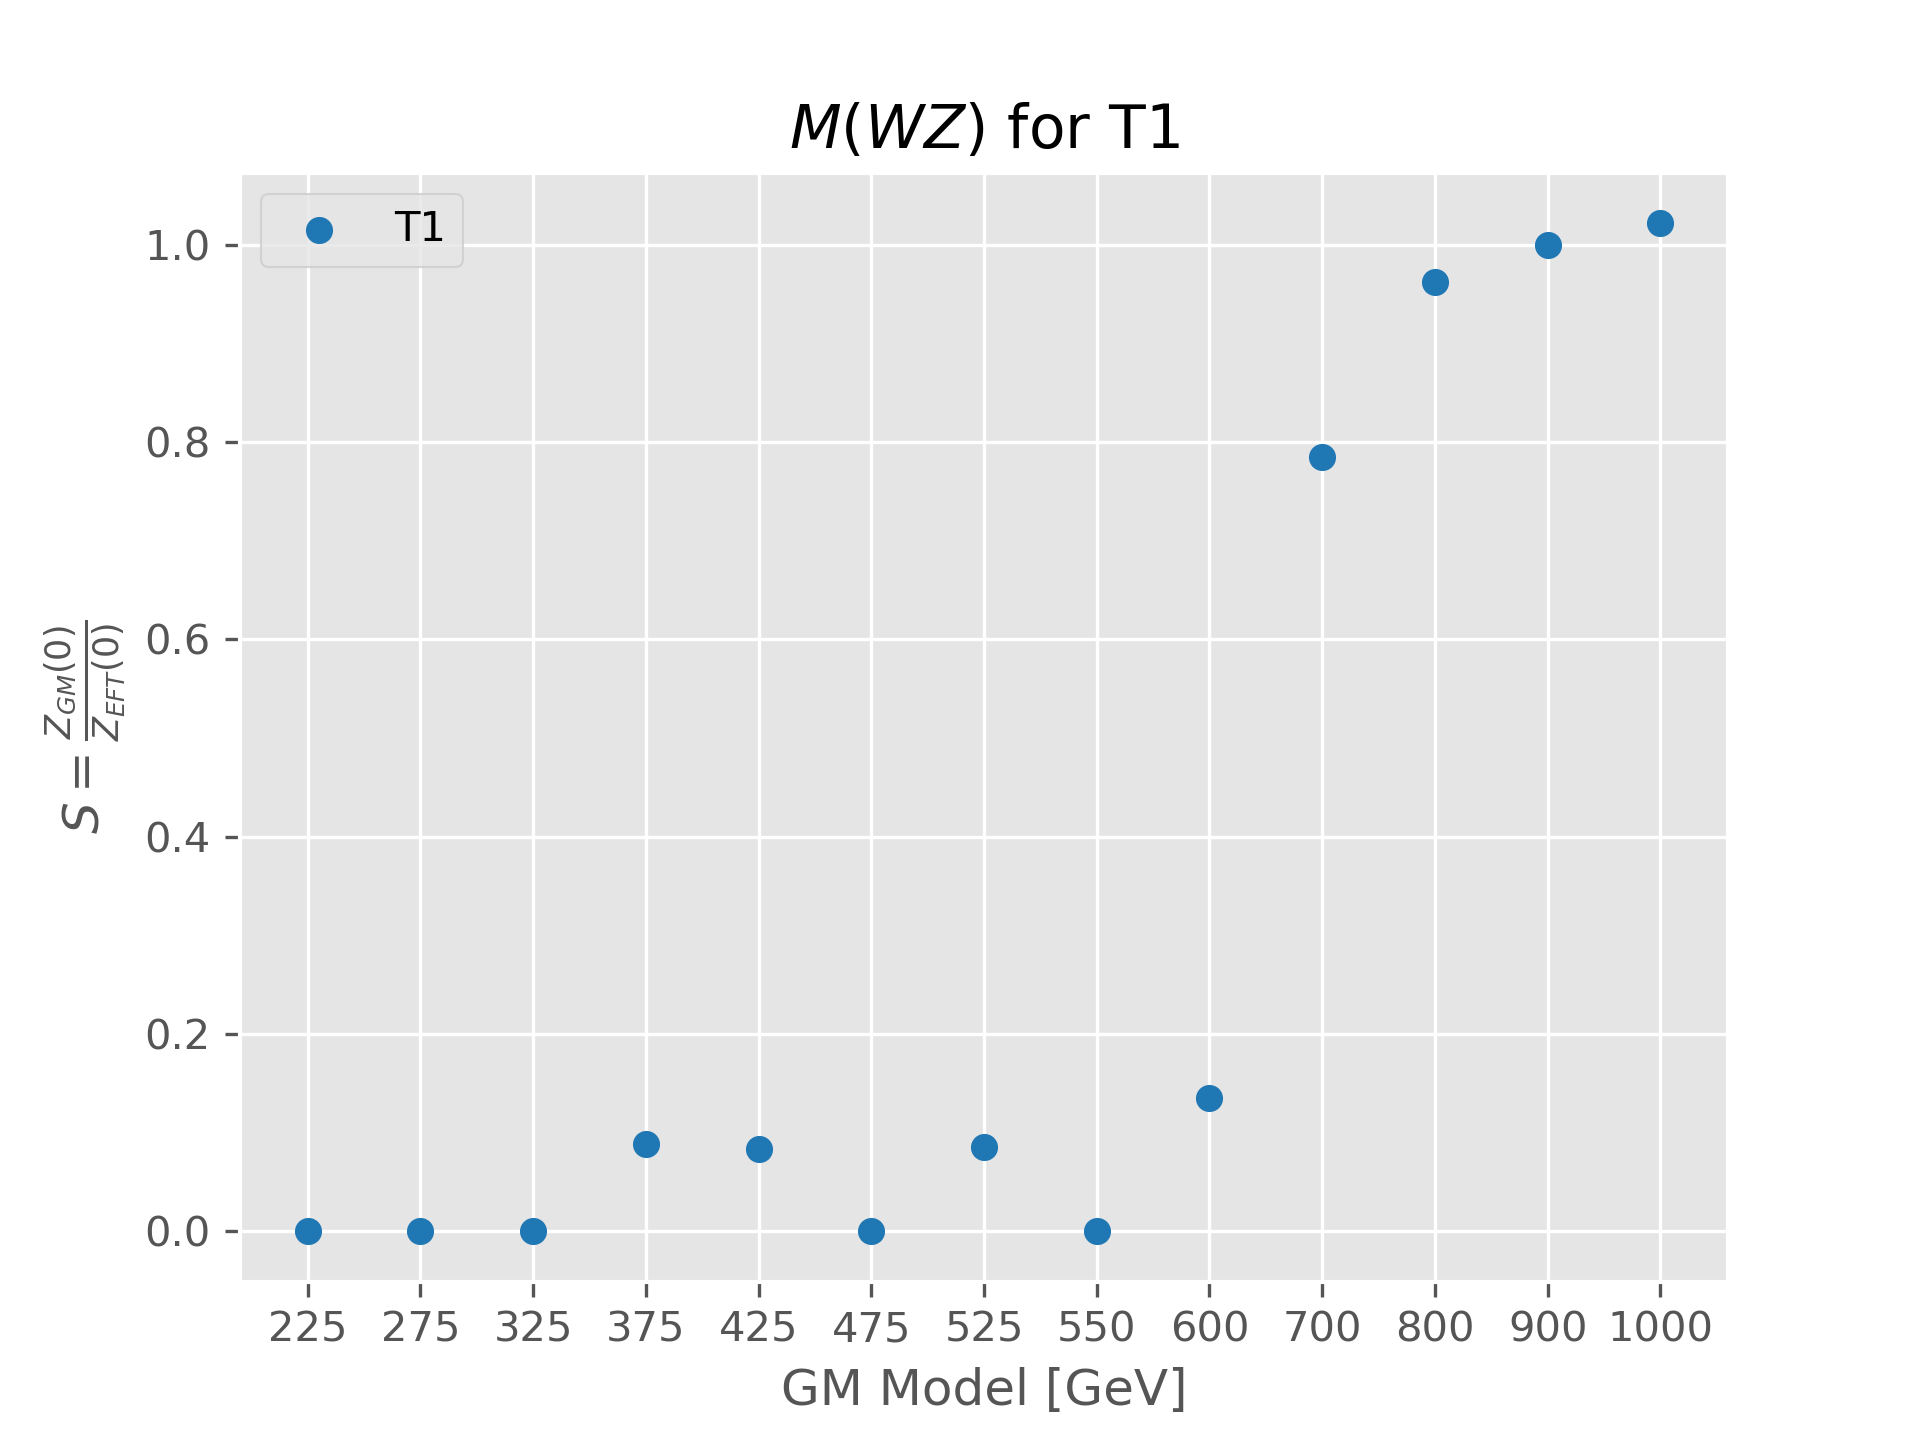
\includegraphics[width=\textwidth]{Plots/gm_relevanze/MWZ_op_T1.png}

    \end{subfigure}
    \begin{subfigure}{0.45\textwidth}
        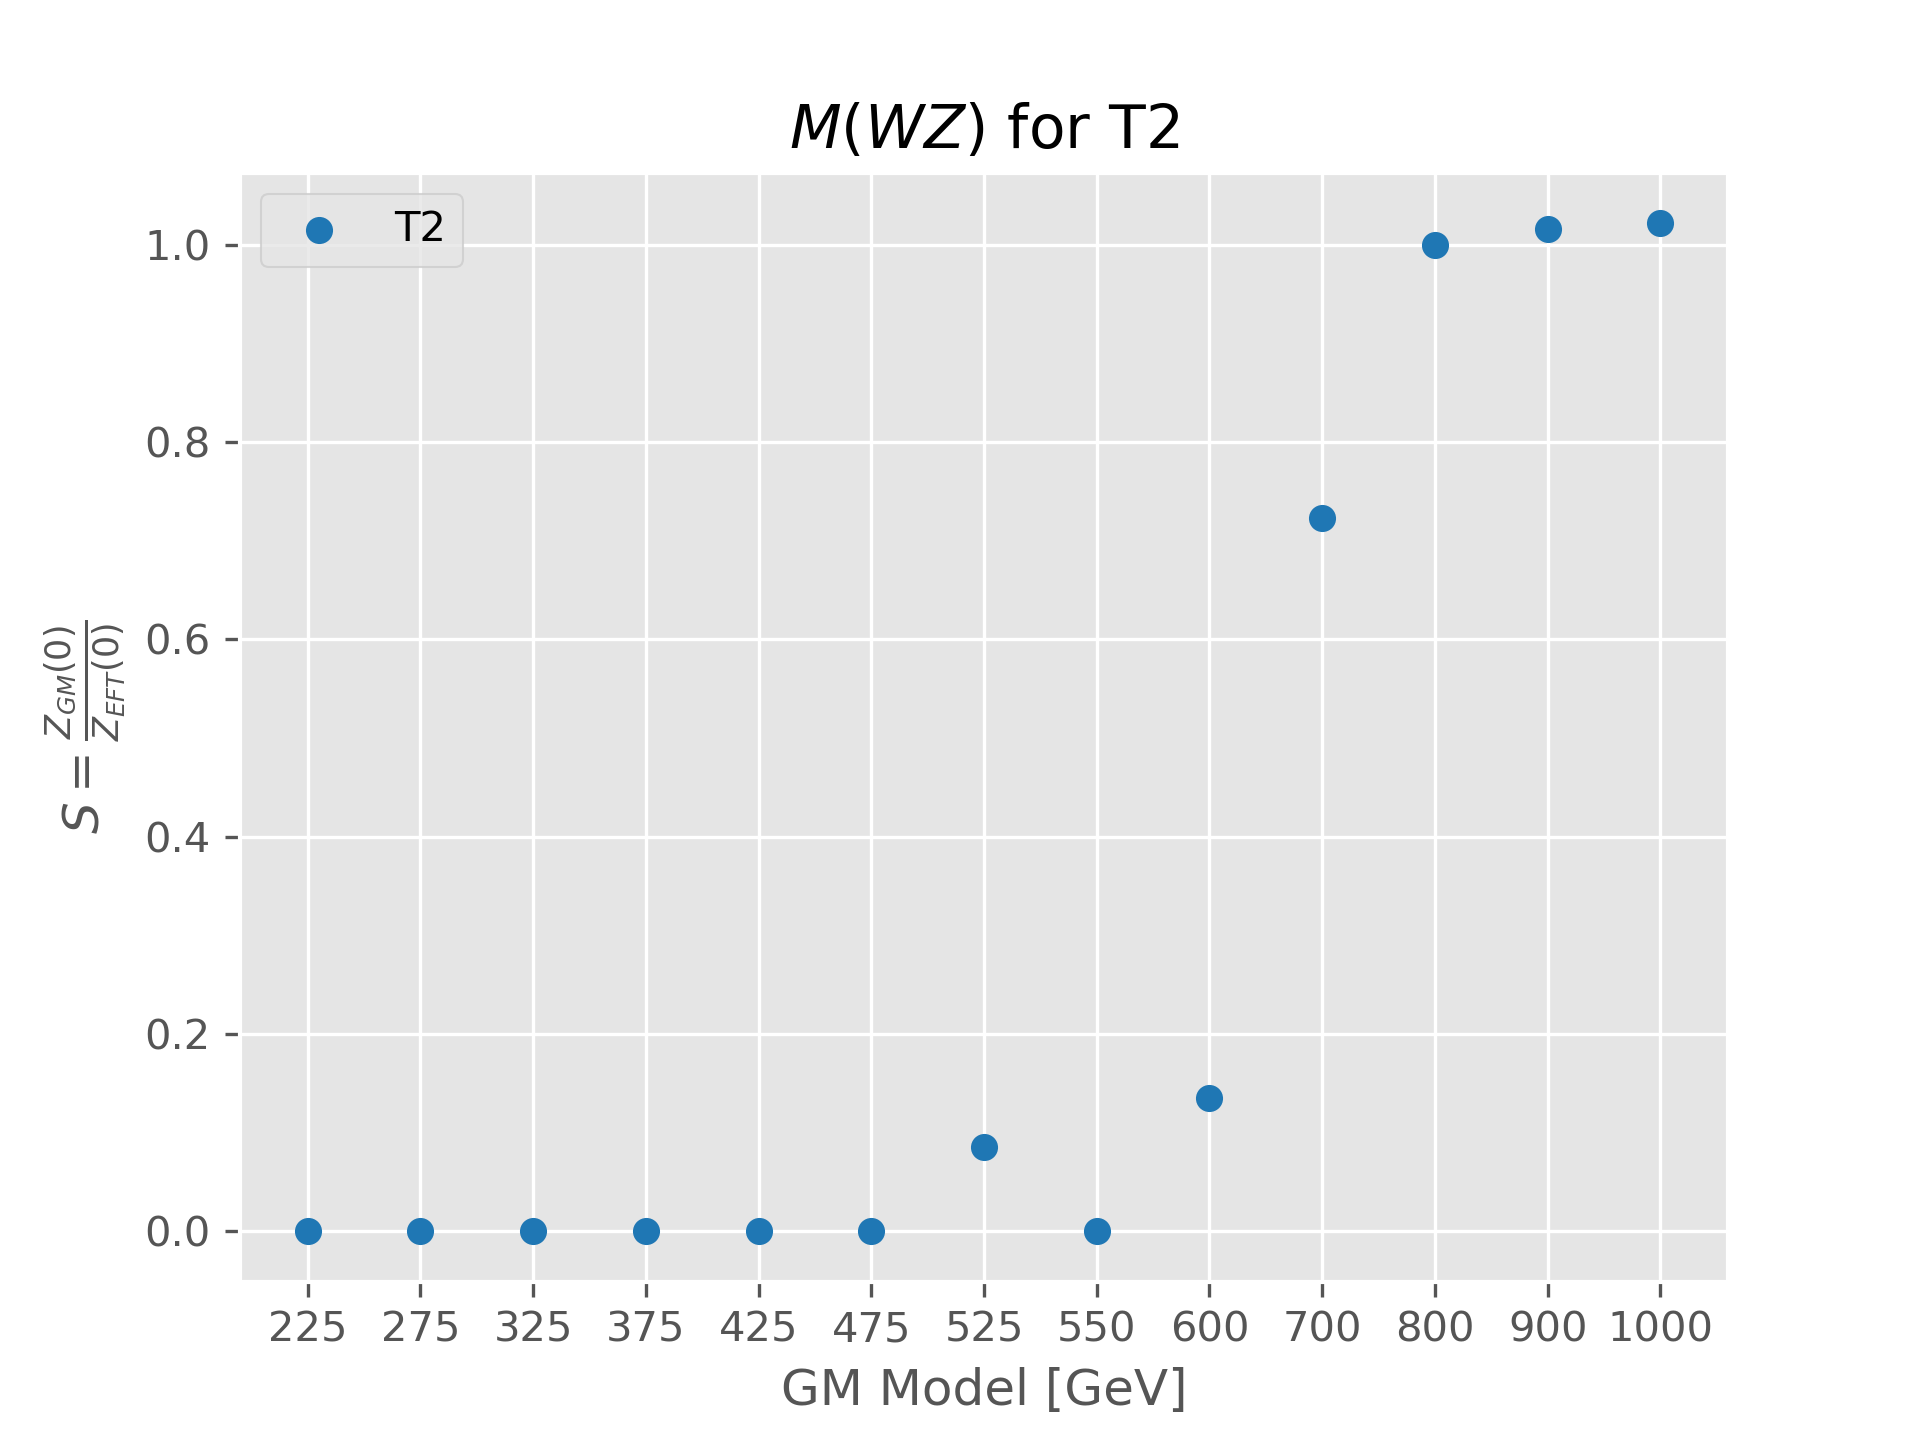
\includegraphics[width=\textwidth]{Plots/gm_relevanze/MWZ_op_T2.png}

    \end{subfigure}

\end{figure}


\begin{figure}[h]
    \centering
    \begin{subfigure}{0.45\textwidth}
        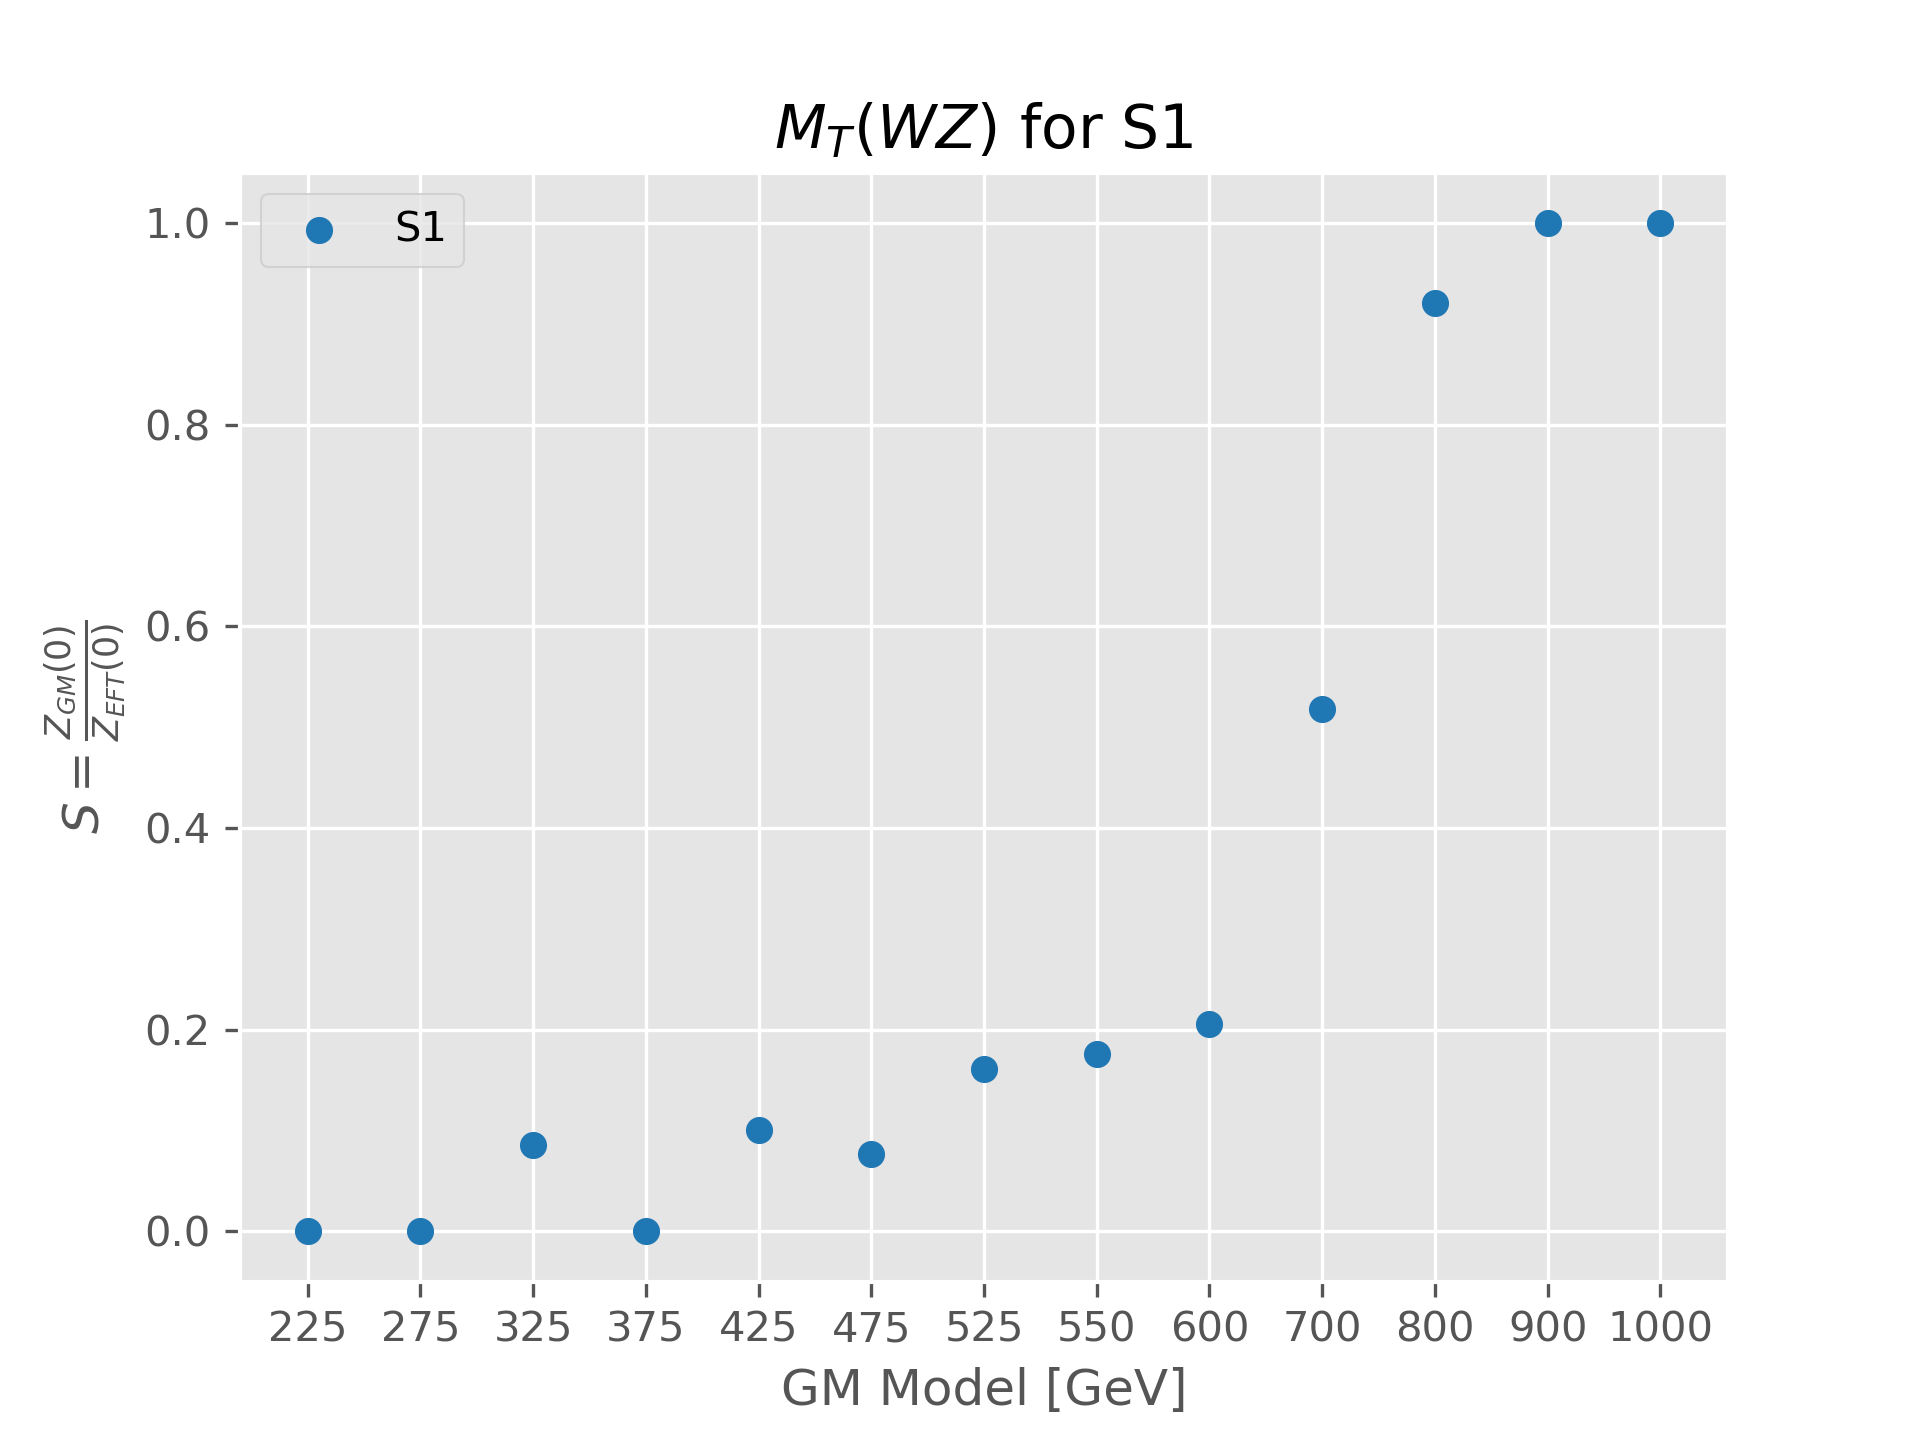
\includegraphics[width=\textwidth]{Plots/gm_relevanze/MTWZ_op_S1.png}

    \end{subfigure}
    \begin{subfigure}{0.45\textwidth}
        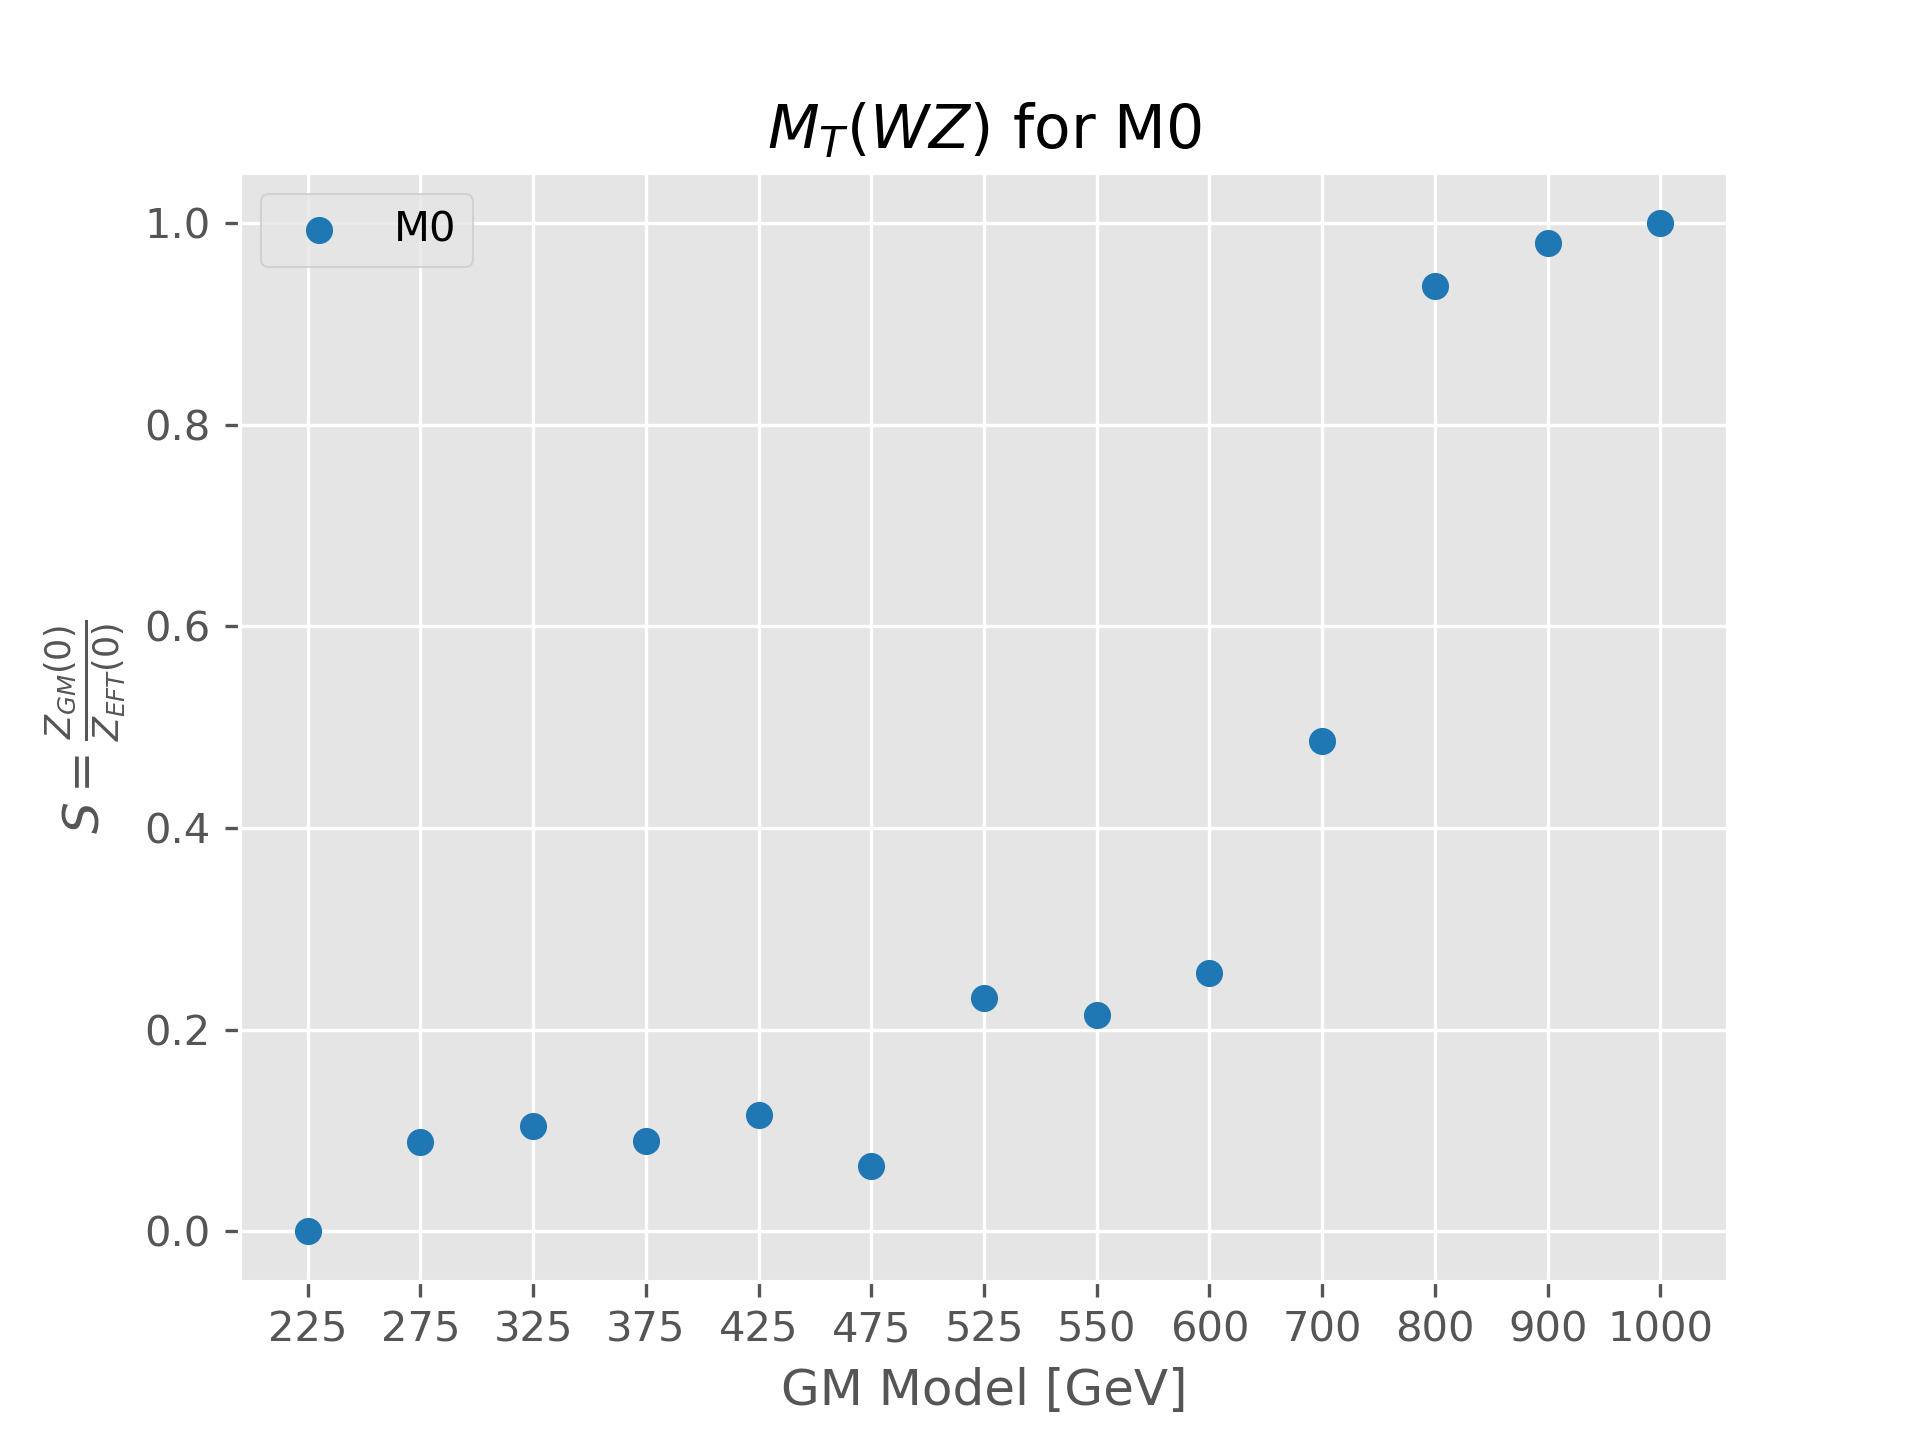
\includegraphics[width=\textwidth]{Plots/gm_relevanze/MTWZ_op_M0.png}

    \end{subfigure}
    \begin{subfigure}{0.45\textwidth}
        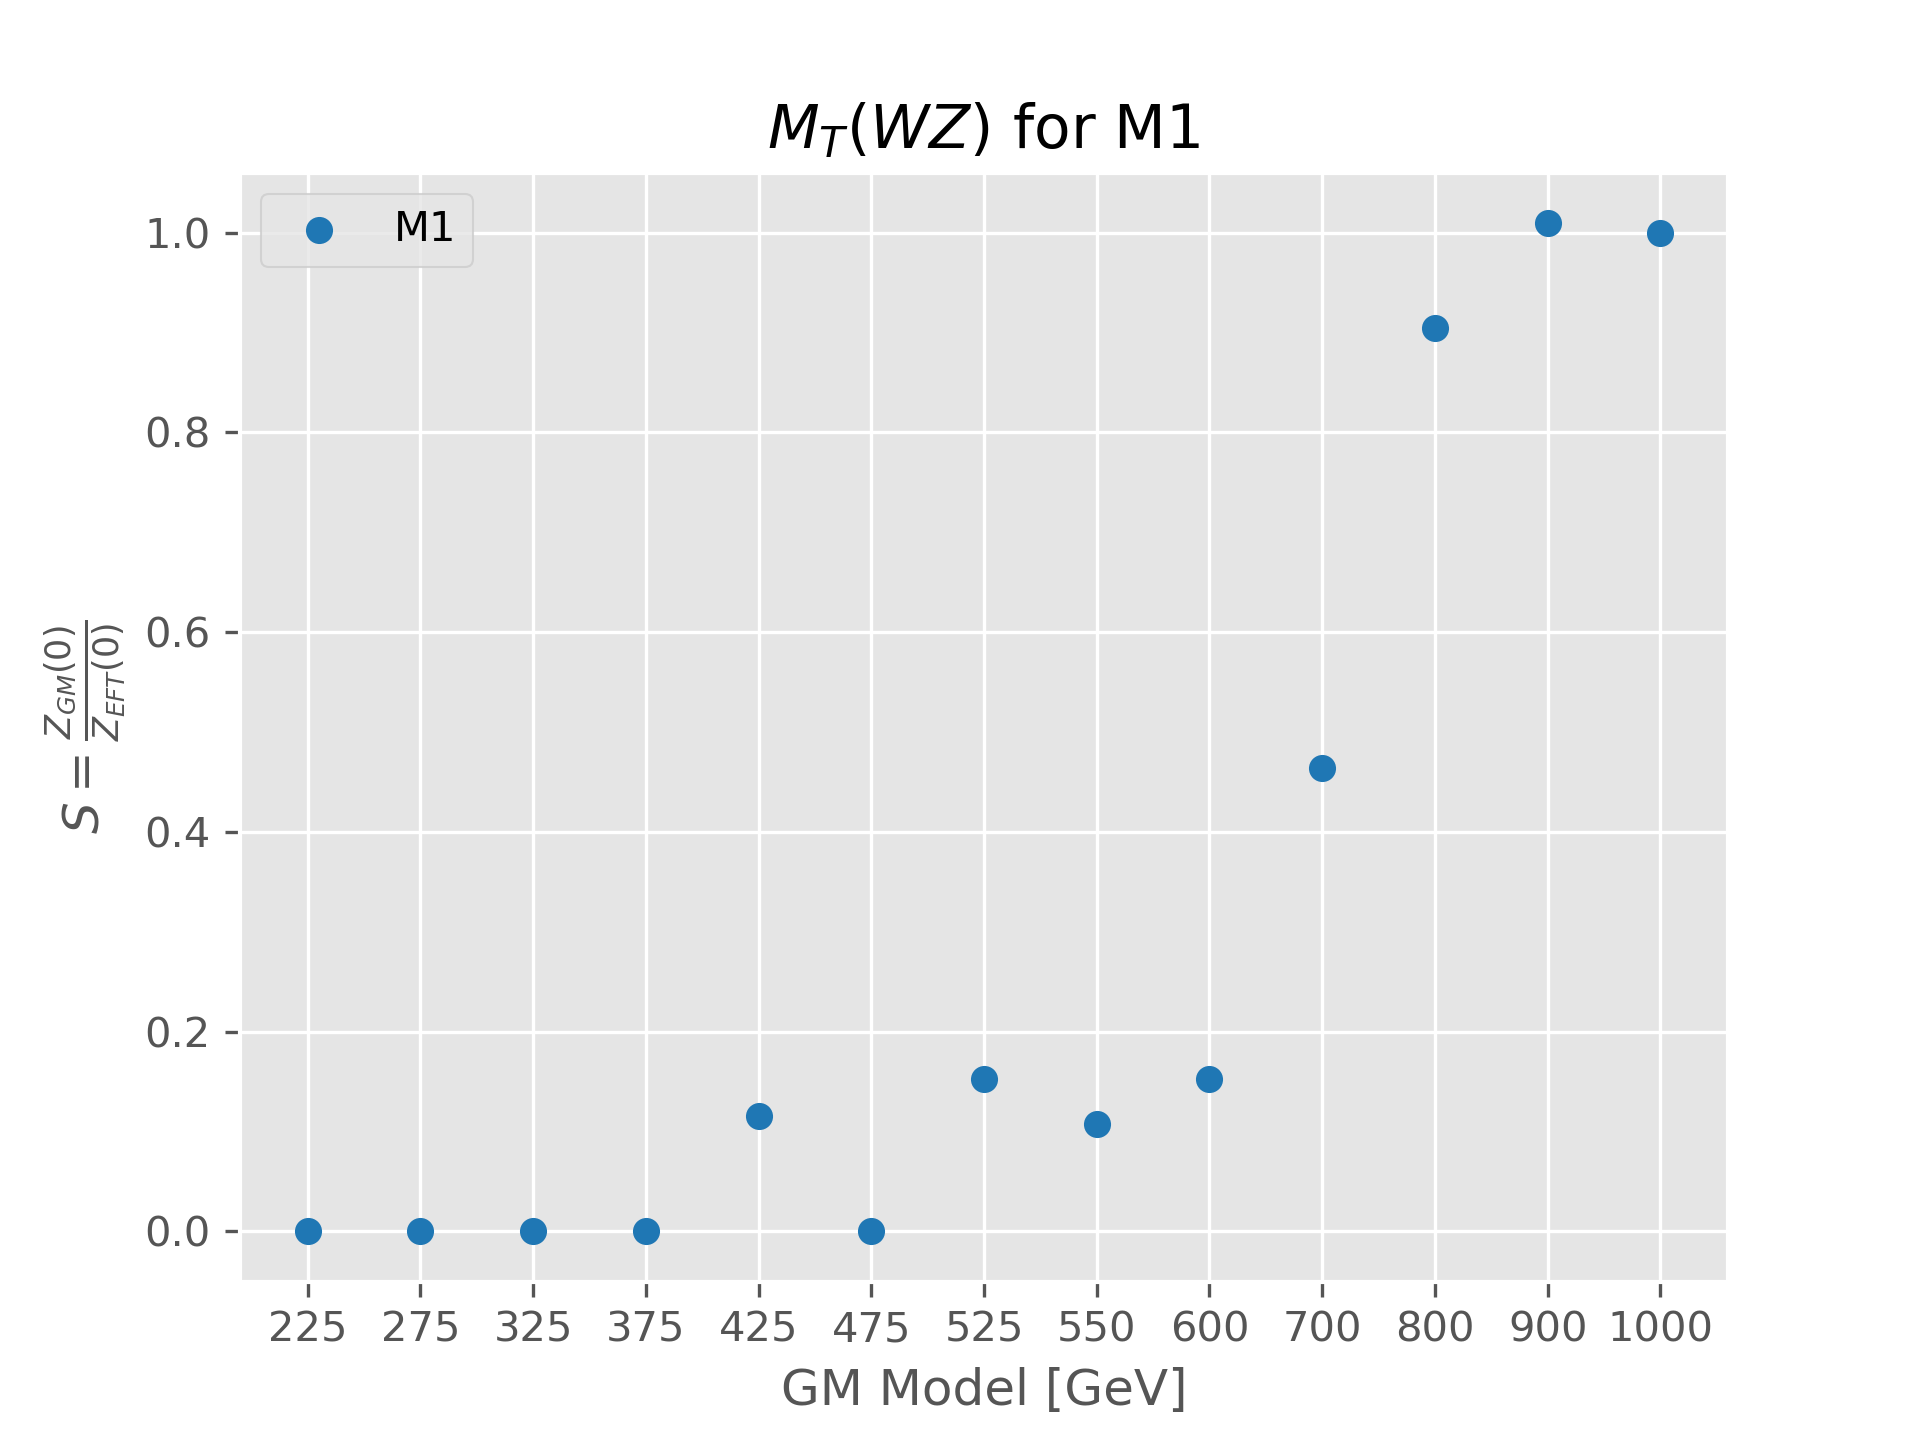
\includegraphics[width=\textwidth]{Plots/gm_relevanze/MTWZ_op_M1.png}

    \end{subfigure}
    \begin{subfigure}{0.45\textwidth}
        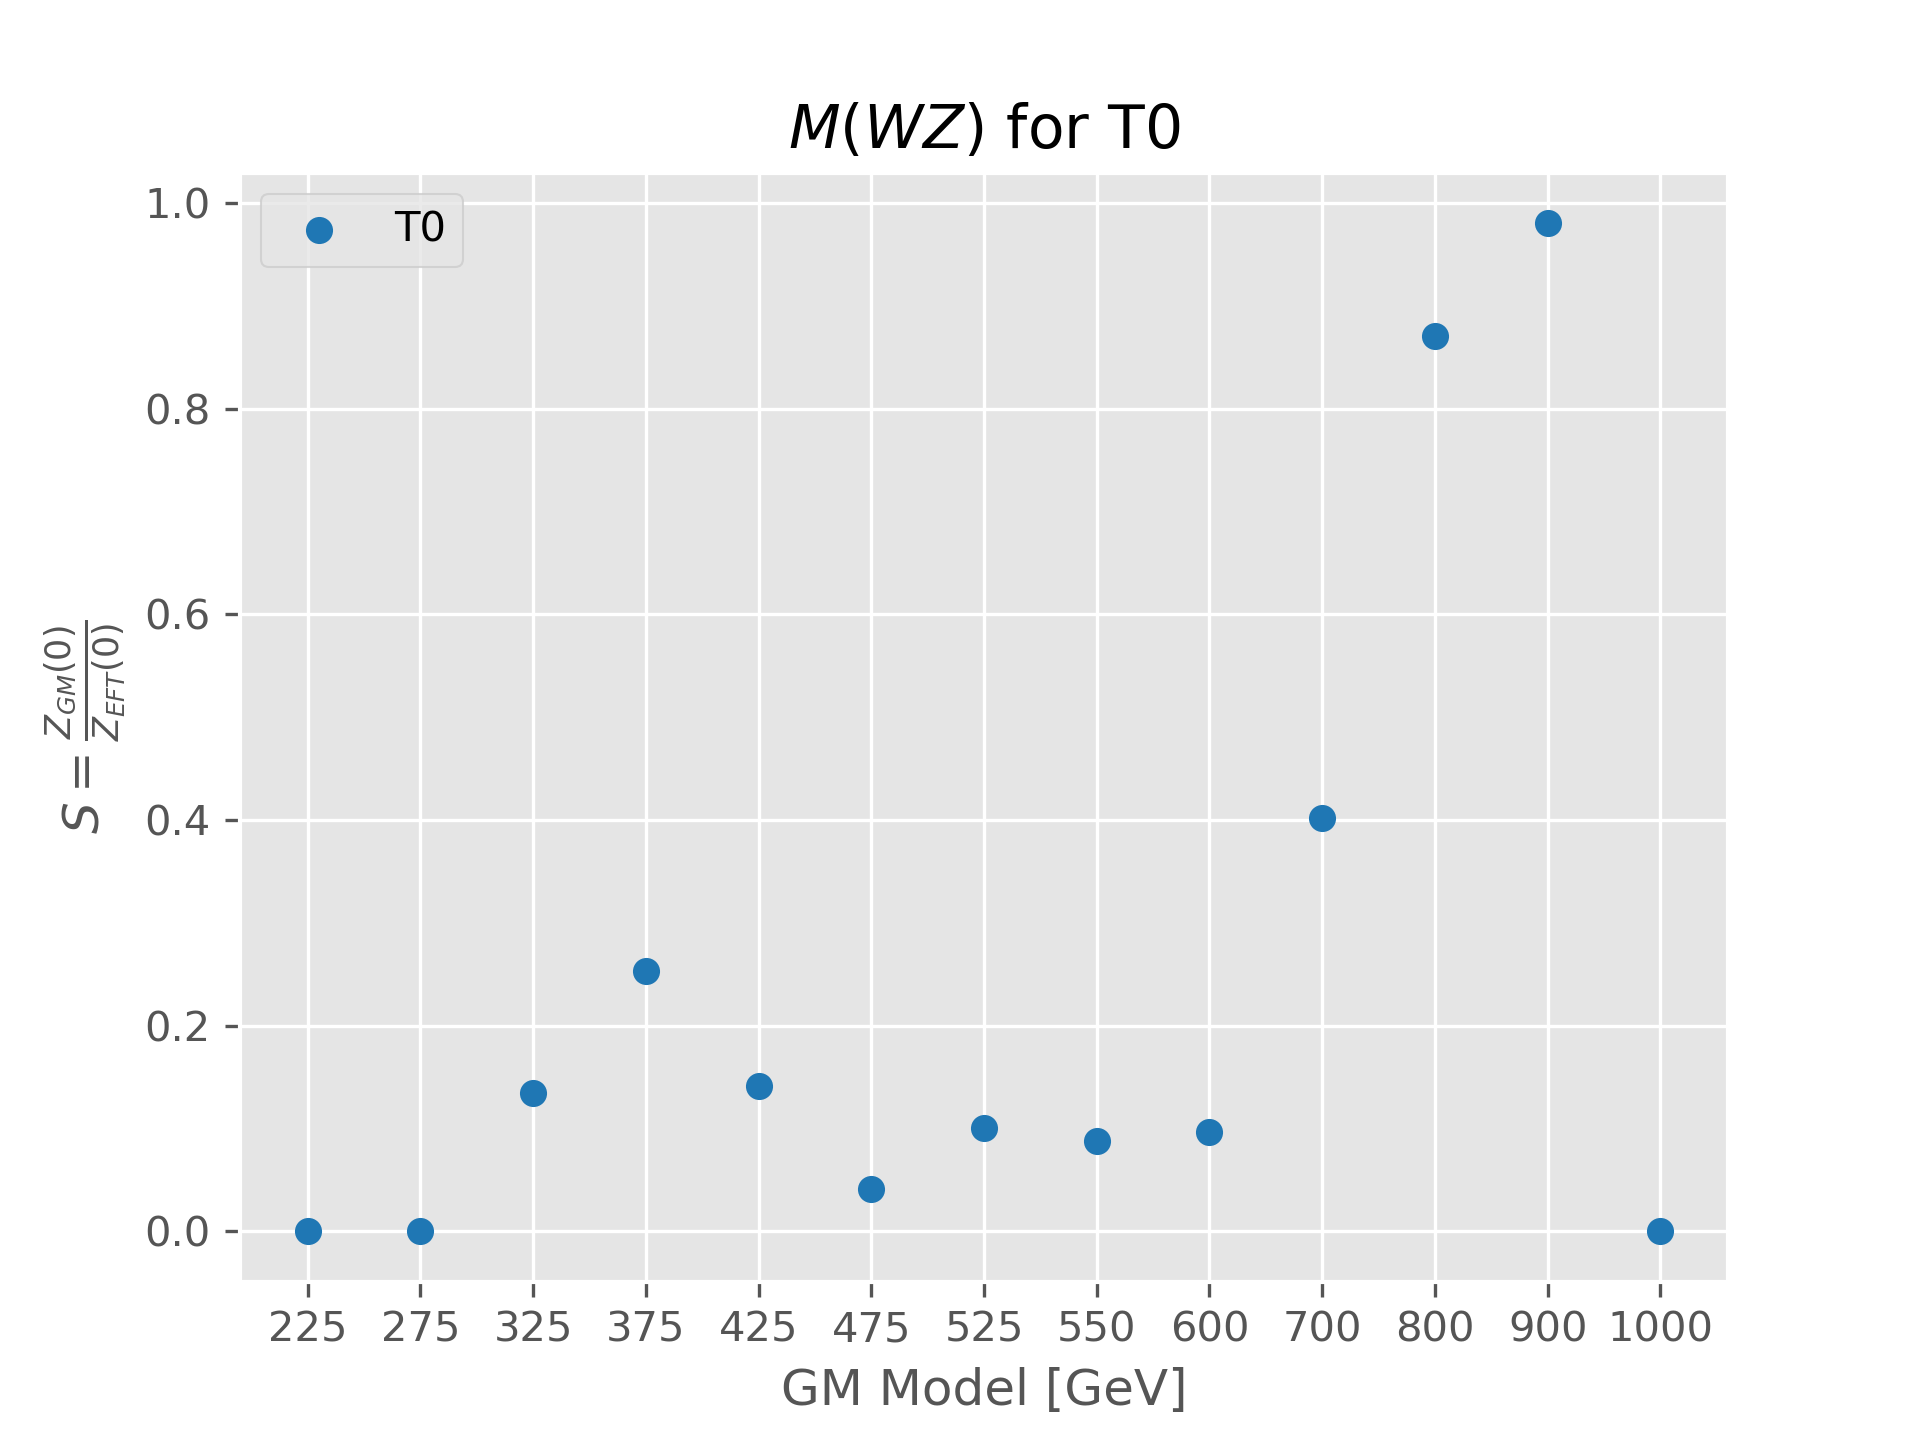
\includegraphics[width=\textwidth]{Plots/gm_relevanze/MTWZ_op_T0.png}

    \end{subfigure}
    \begin{subfigure}{0.45\textwidth}
        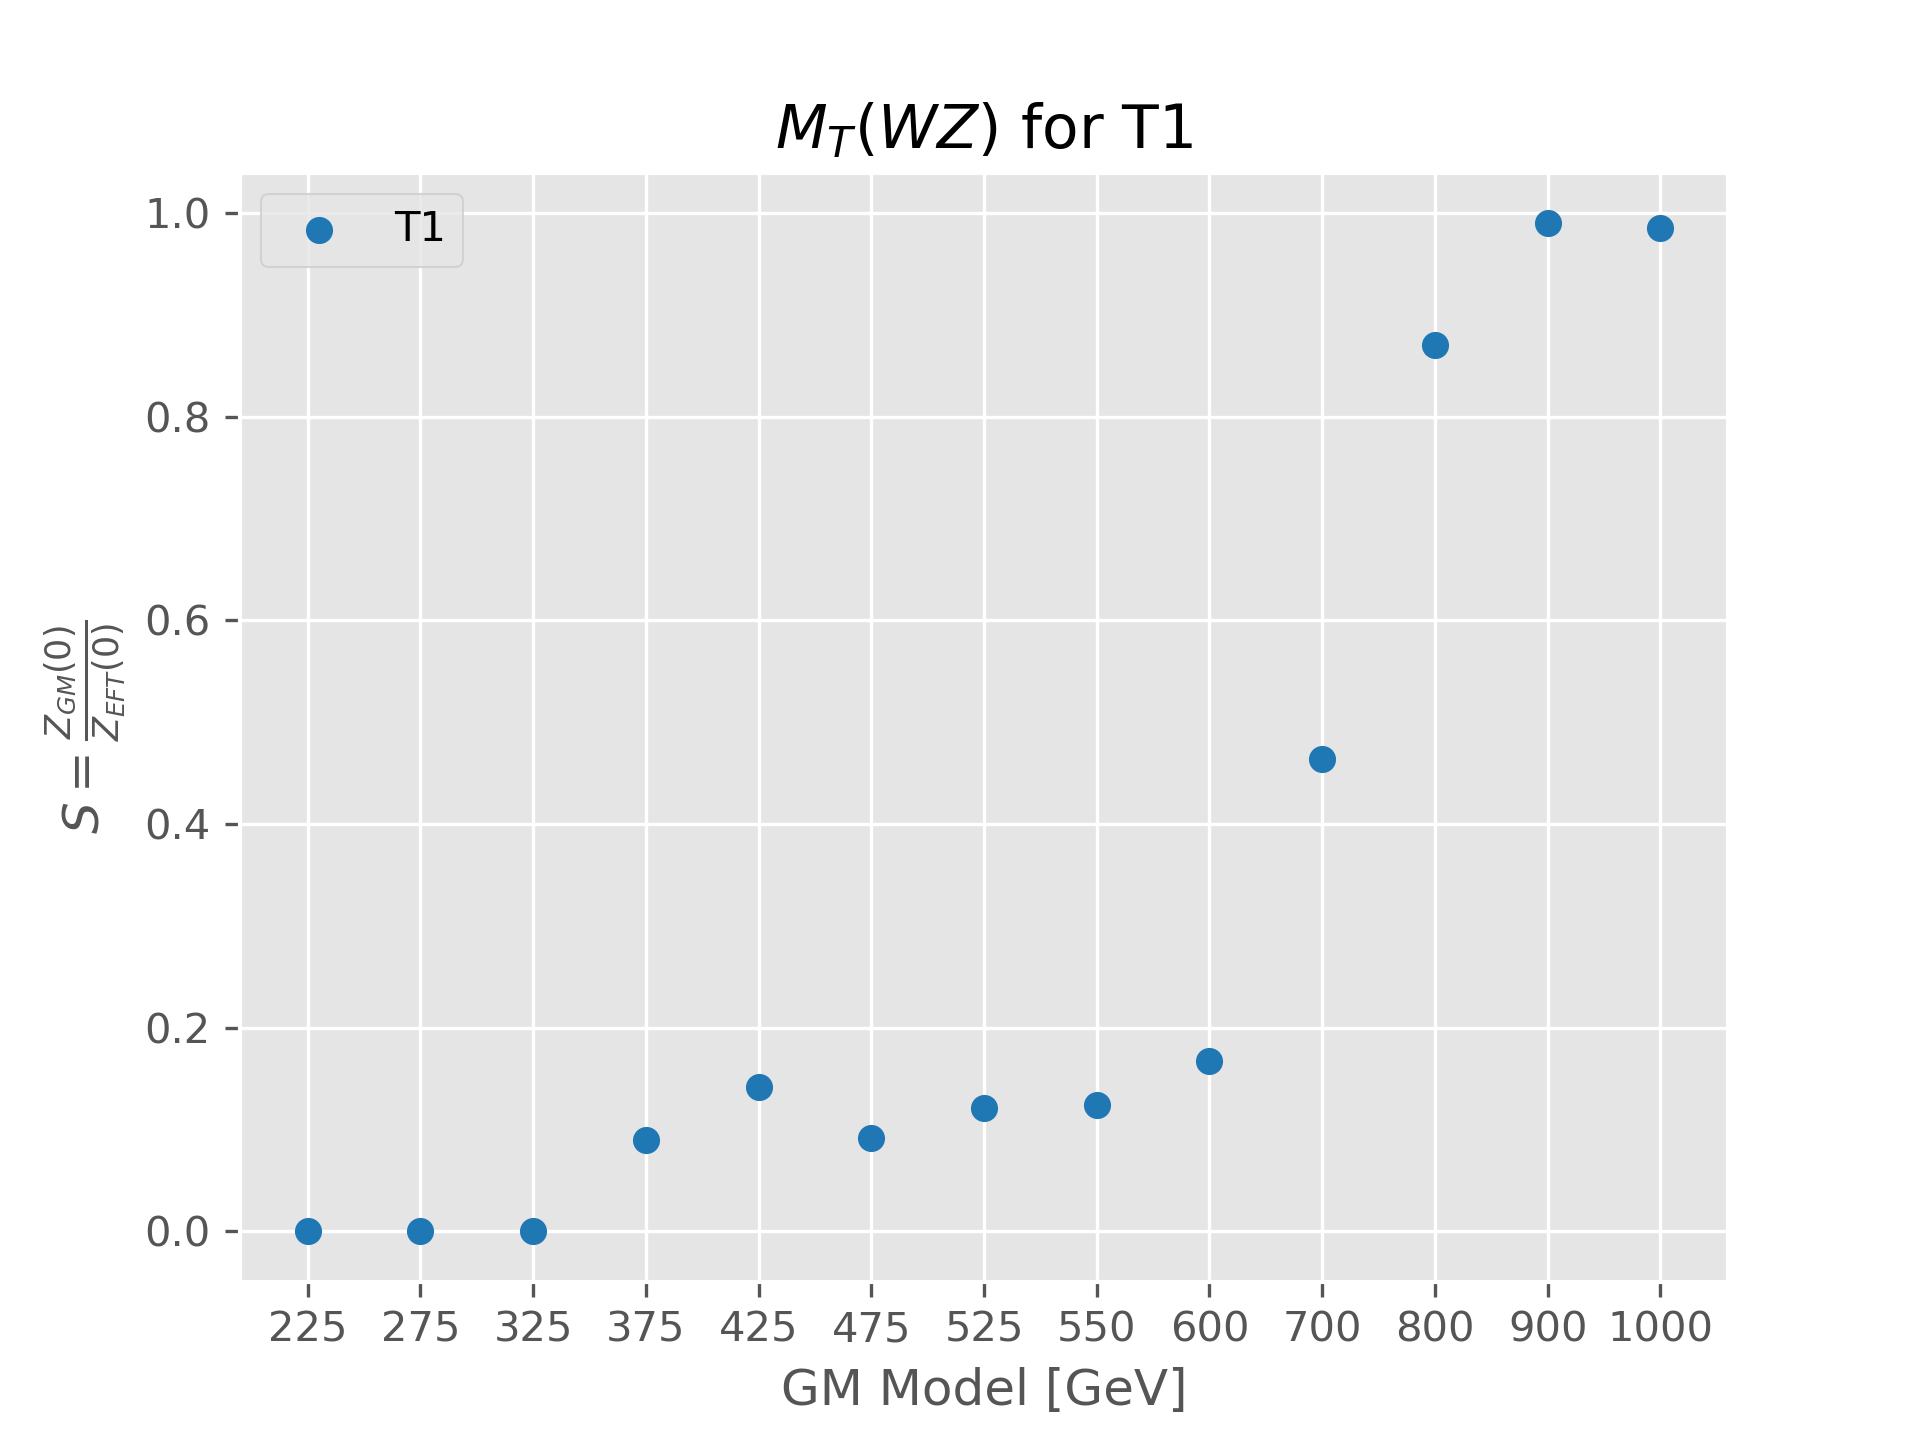
\includegraphics[width=\textwidth]{Plots/gm_relevanze/MTWZ_op_T1.png}

    \end{subfigure}
    \begin{subfigure}{0.45\textwidth}
        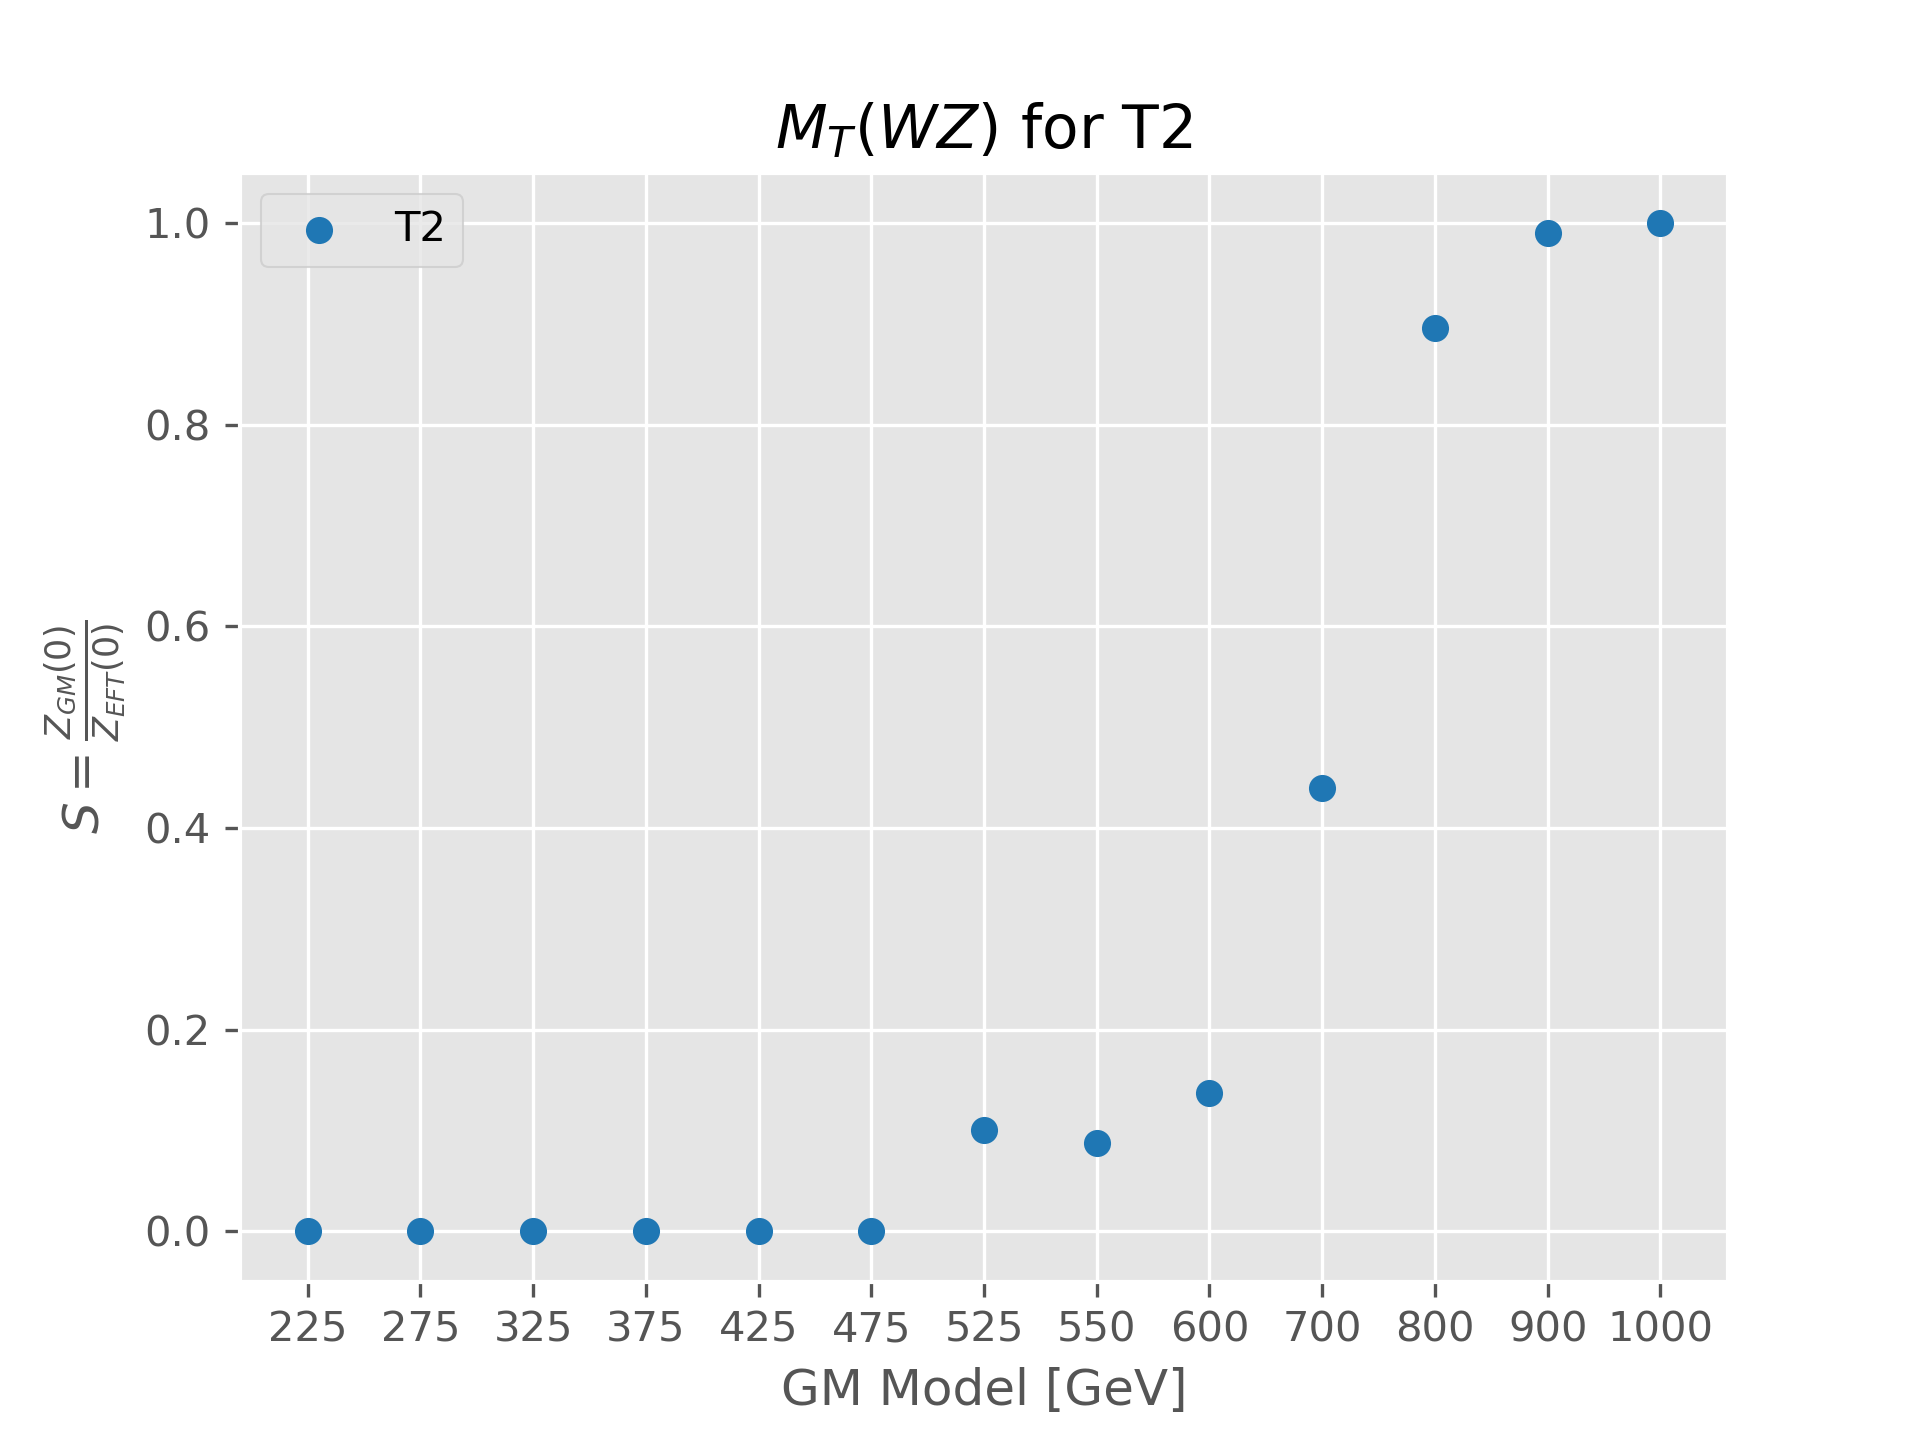
\includegraphics[width=\textwidth]{Plots/gm_relevanze/MTWZ_op_T2.png}

    \end{subfigure}

\end{figure}


\section{Cross-section comparison for dim-8 operators}
\label{sec:cross-section-comp}
\begin{figure}[h]
    \centering
    \begin{subfigure}{0.45\textwidth}
        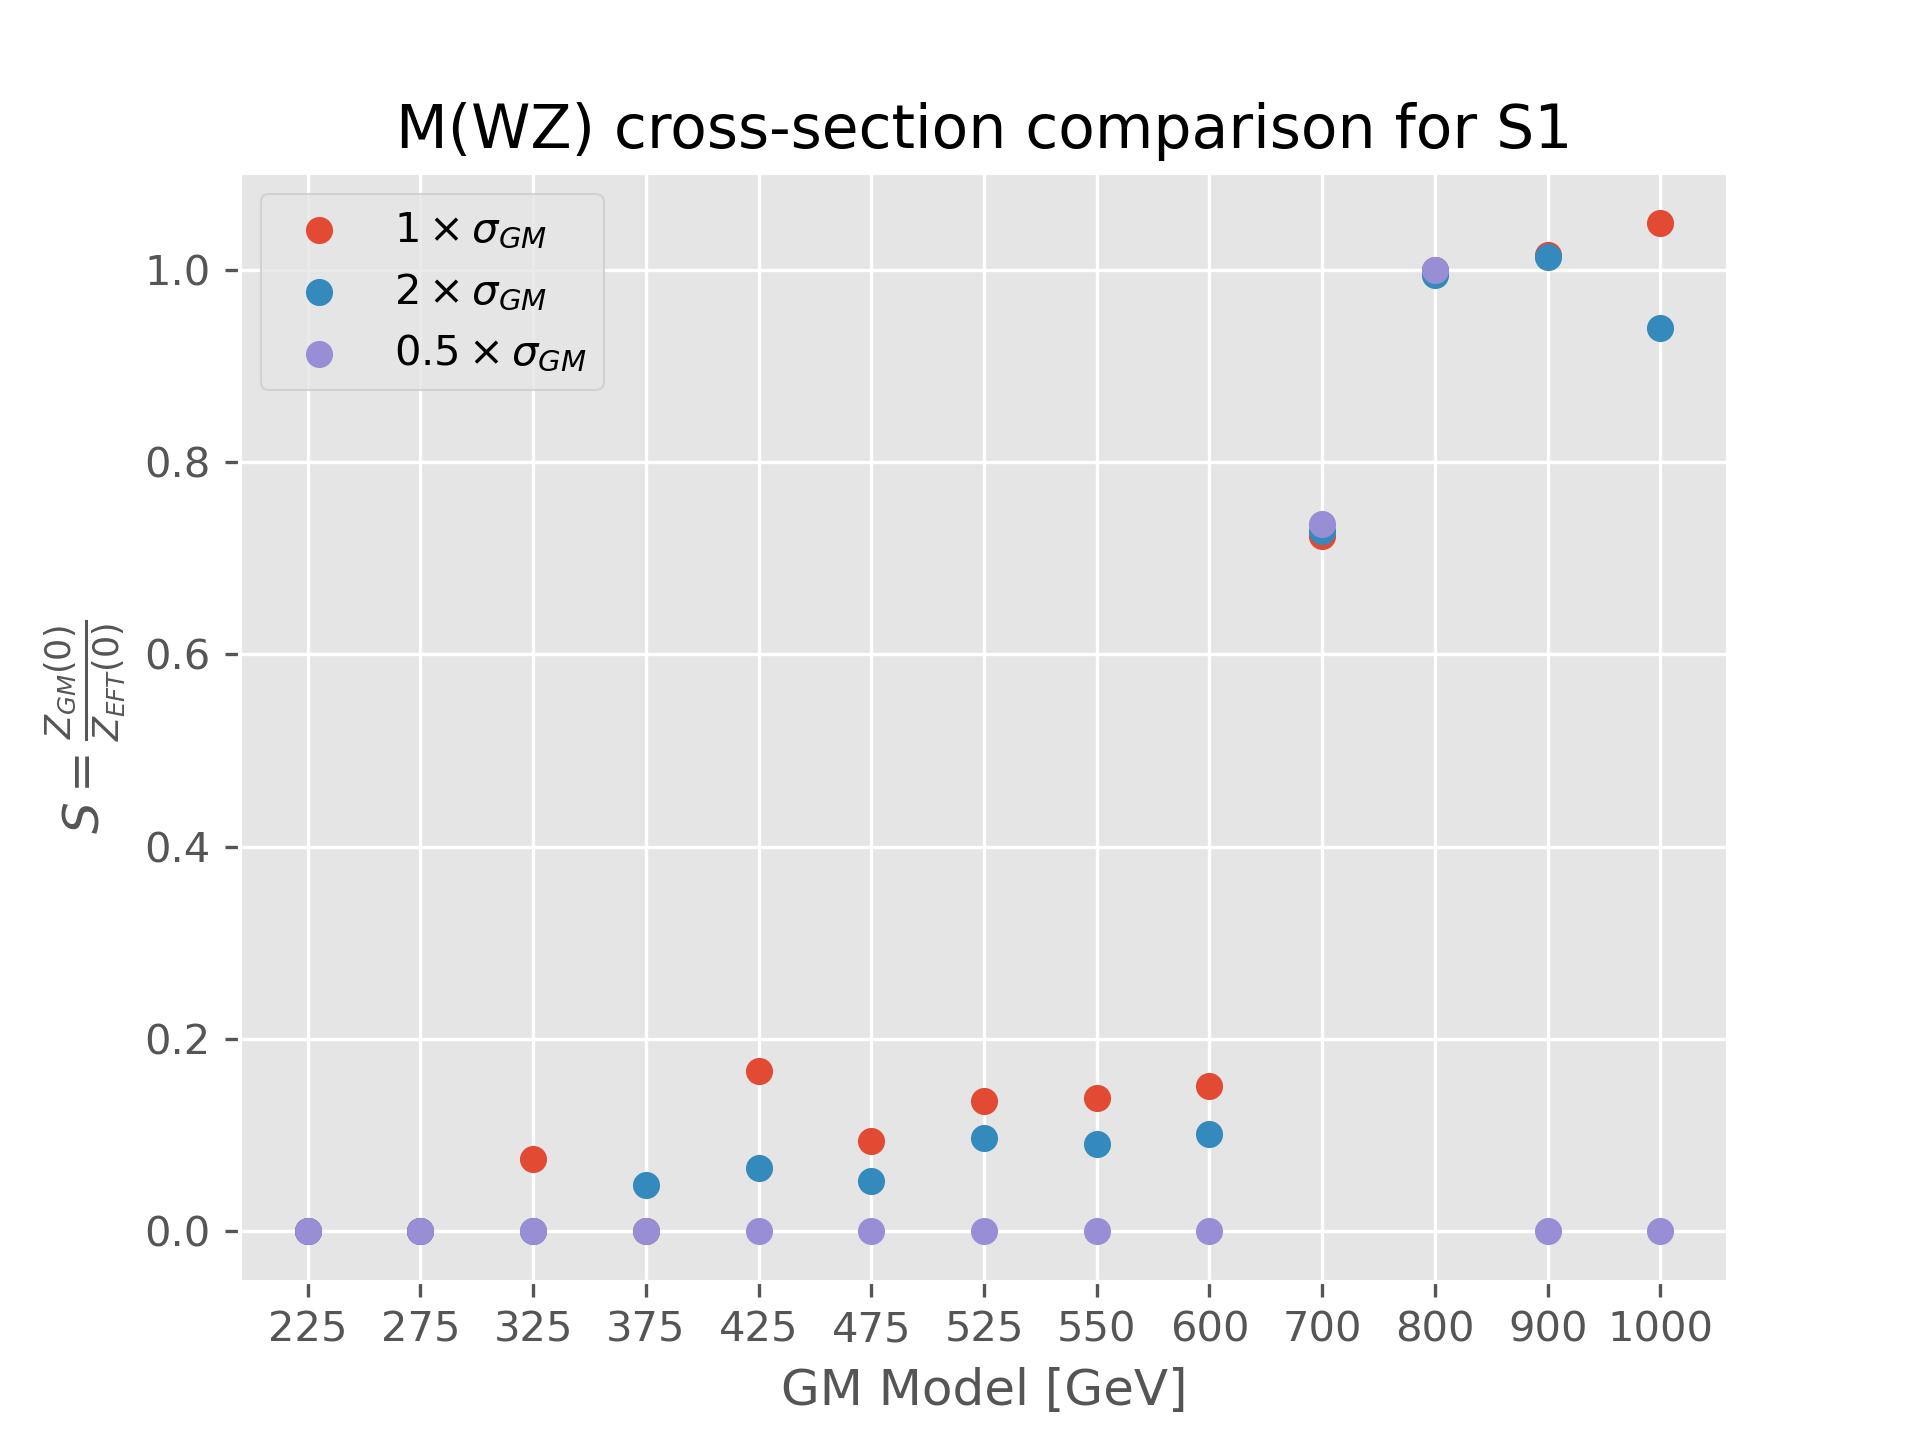
\includegraphics[width=\textwidth]{Plots/gm_relevanze/MWZ_comparision_S1.png}

    \end{subfigure}
    \begin{subfigure}{0.45\textwidth}
        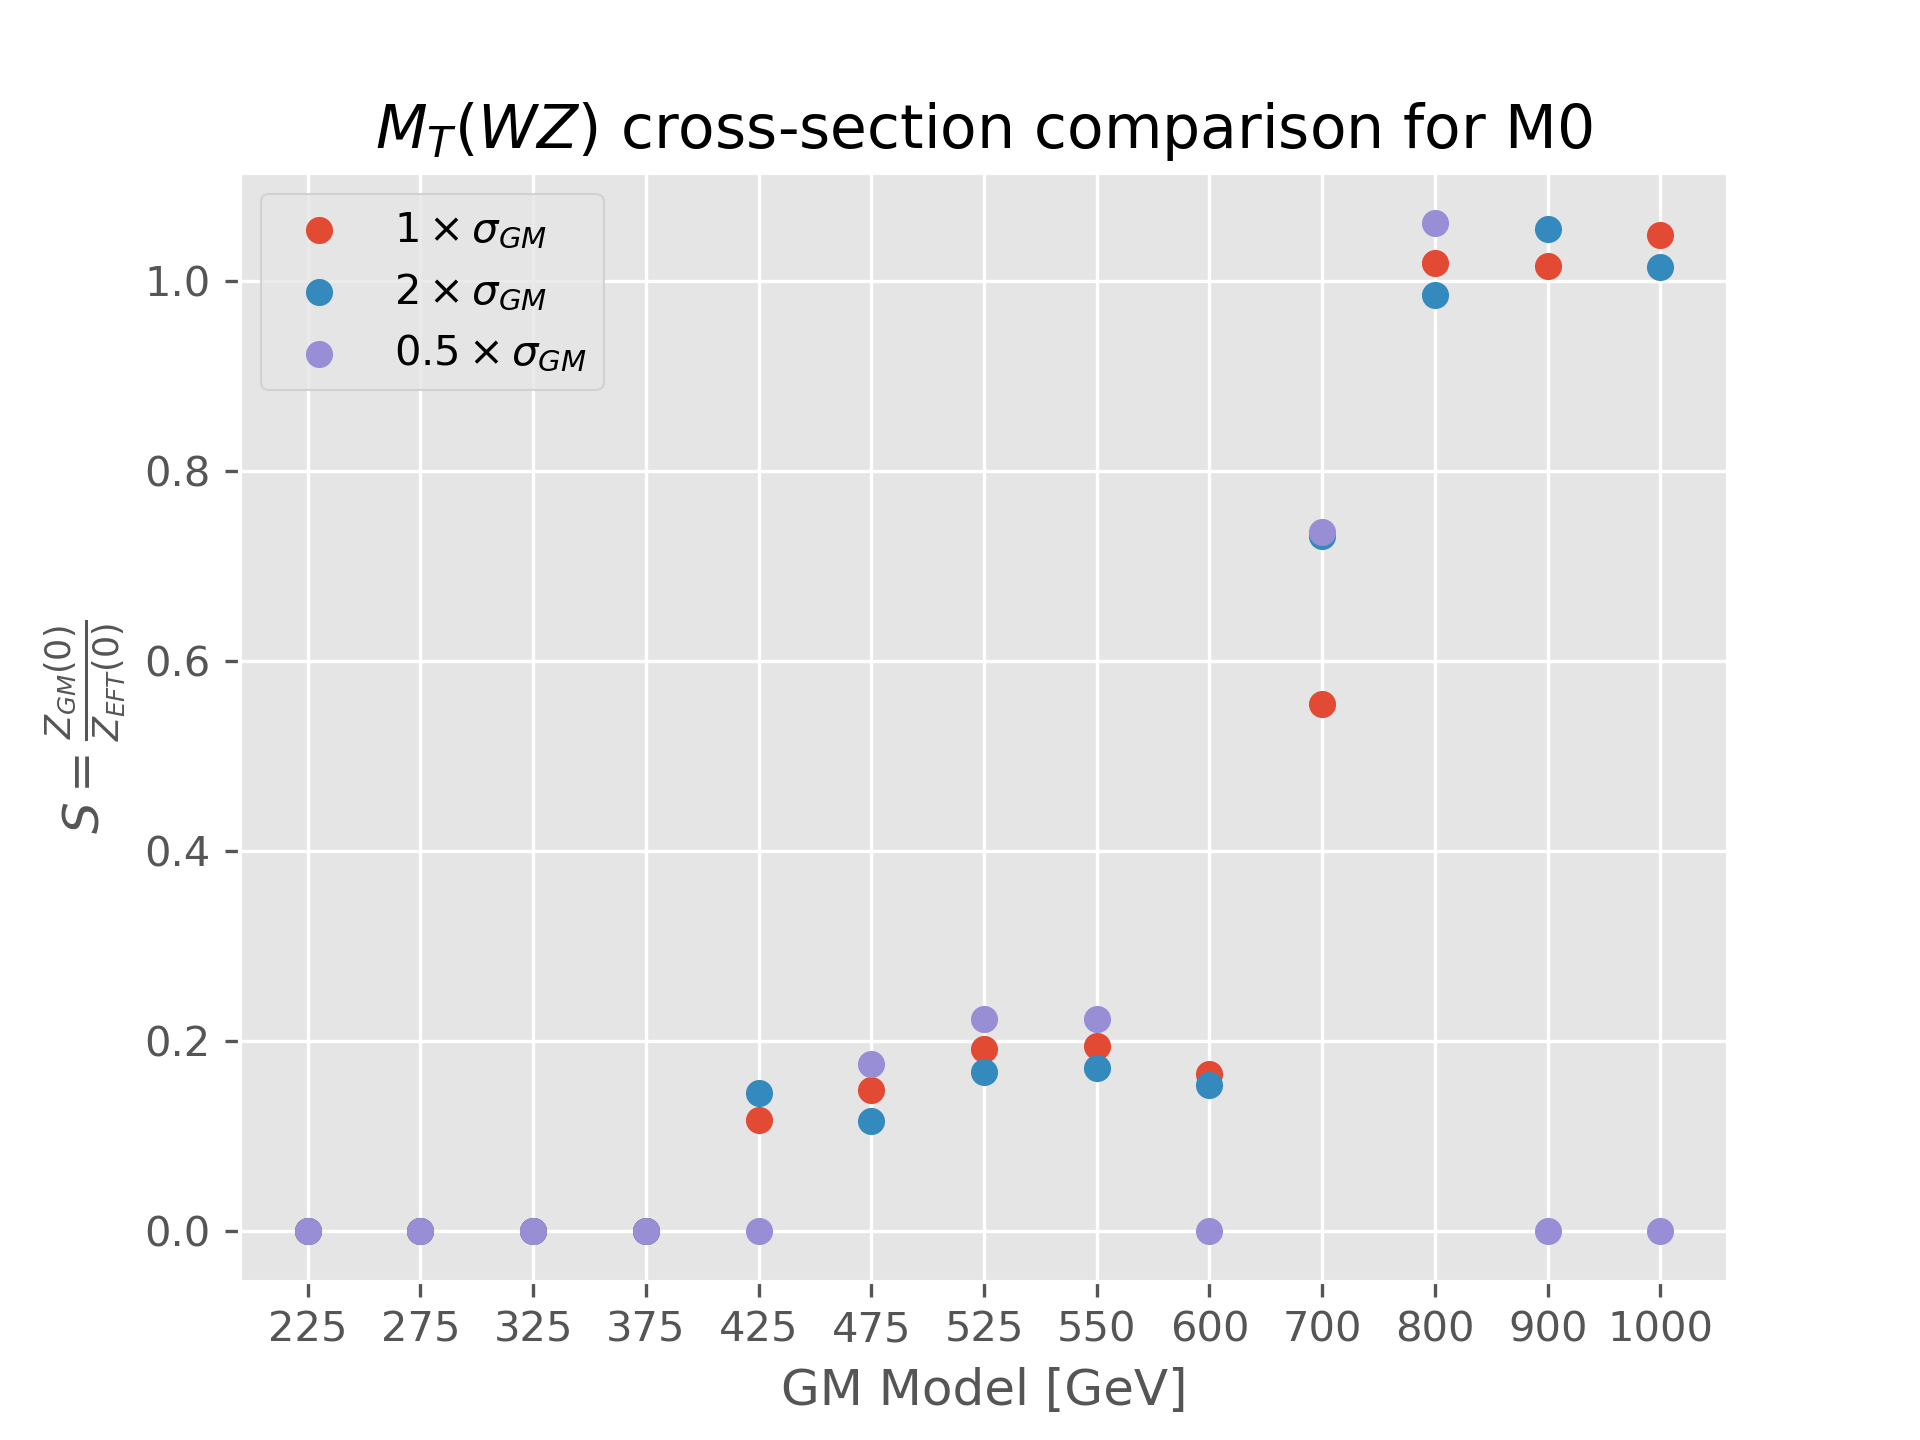
\includegraphics[width=\textwidth]{Plots/gm_relevanze/MWZ_comparision_M0.png}

    \end{subfigure}
    \begin{subfigure}{0.45\textwidth}
        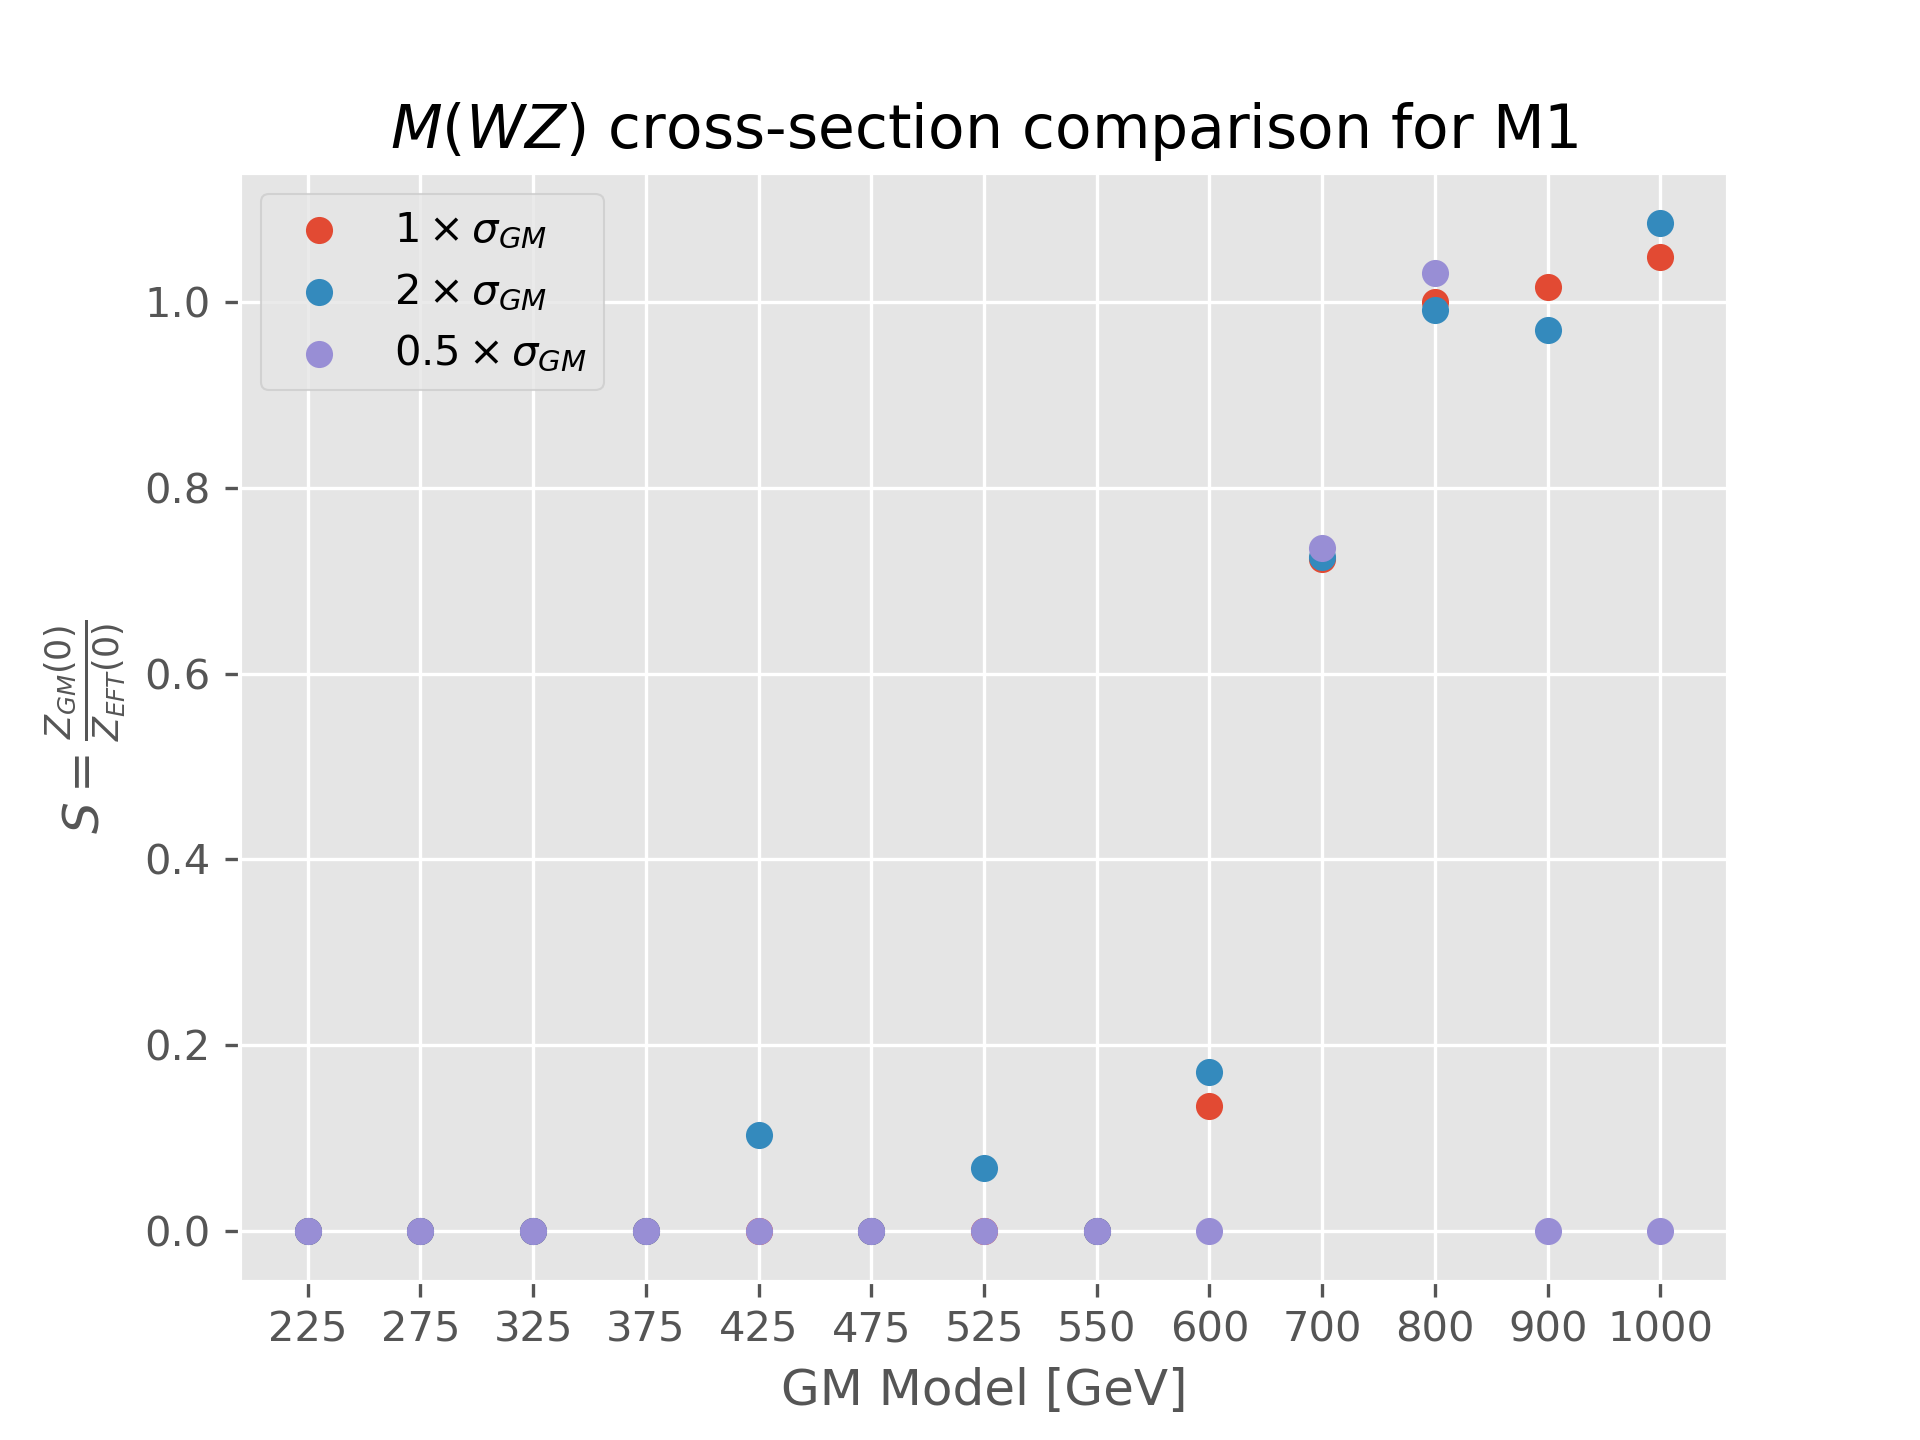
\includegraphics[width=\textwidth]{Plots/gm_relevanze/MWZ_comparision_M1.png}

    \end{subfigure}
    \begin{subfigure}{0.45\textwidth}
        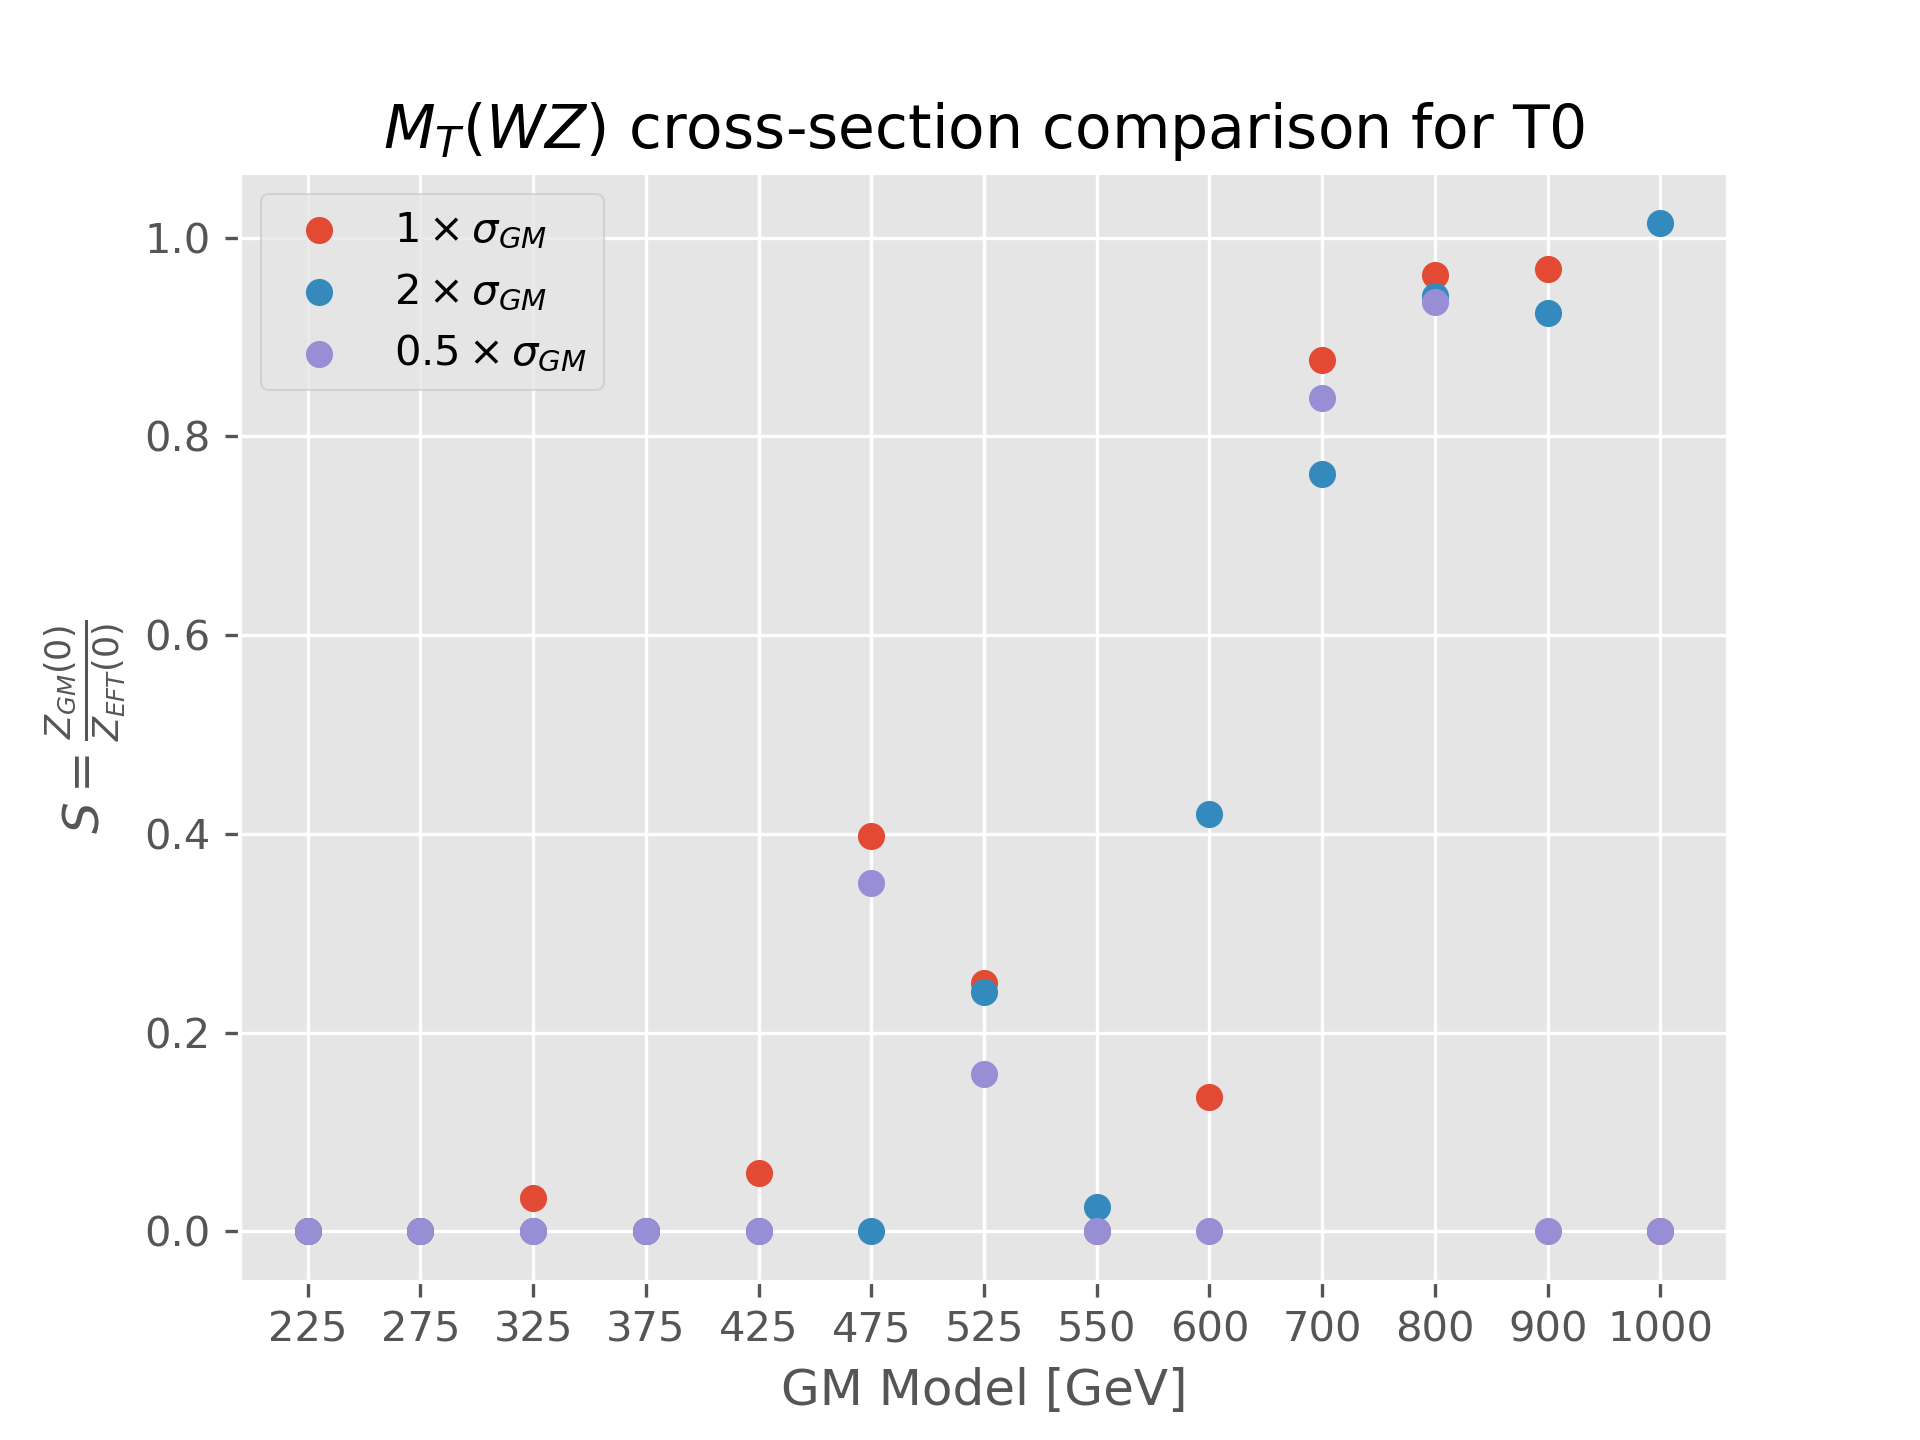
\includegraphics[width=\textwidth]{Plots/gm_relevanze/MWZ_comparision_T0.png}

    \end{subfigure}
    \begin{subfigure}{0.45\textwidth}
        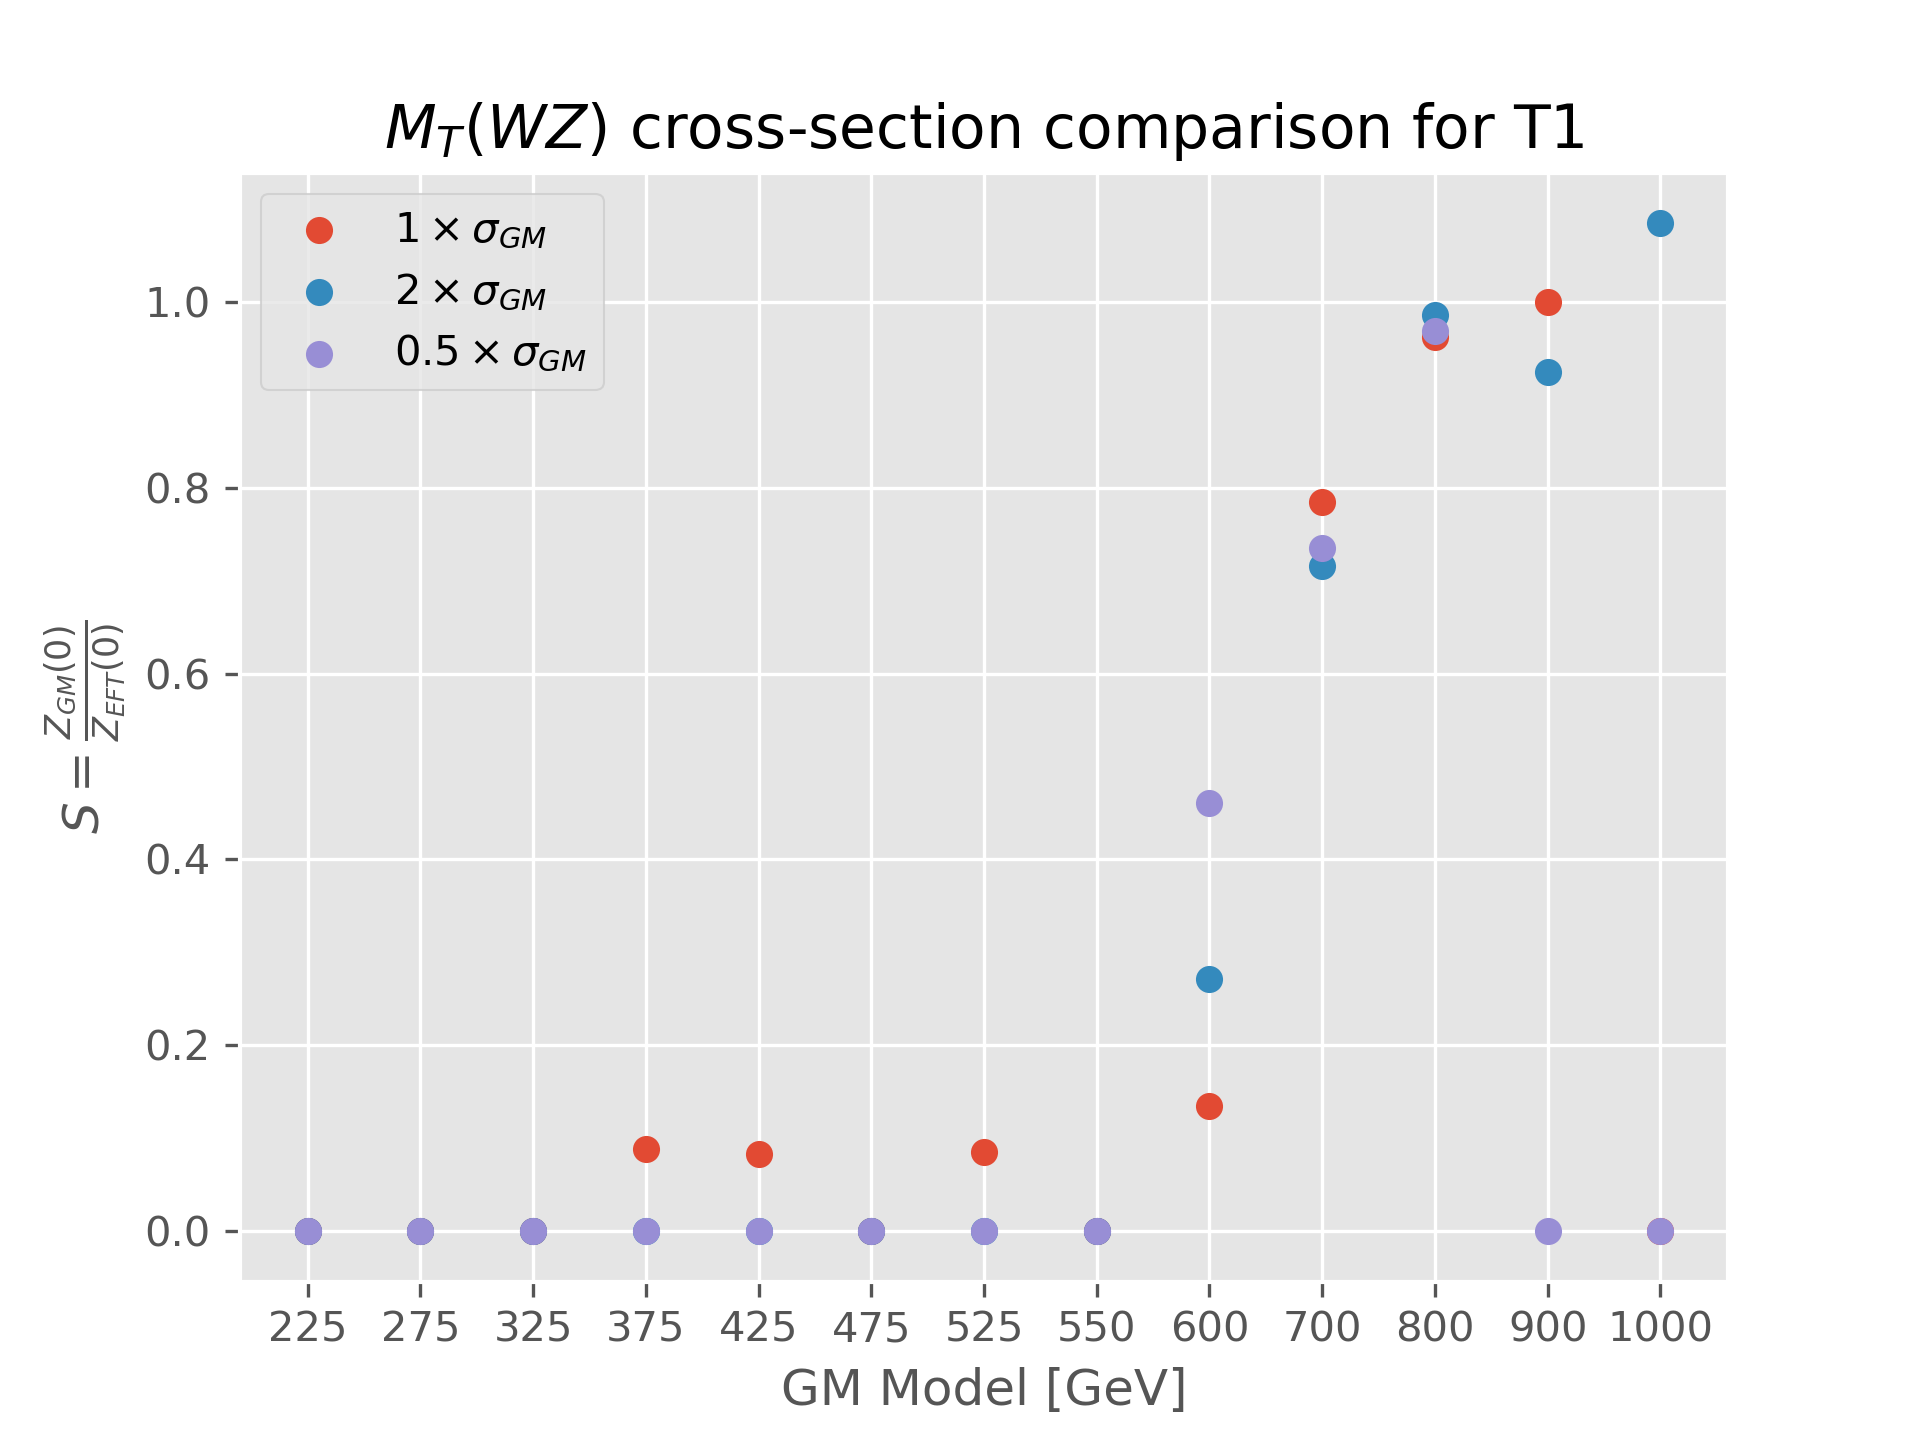
\includegraphics[width=\textwidth]{Plots/gm_relevanze/MWZ_comparision_T1.png}

    \end{subfigure}
    \begin{subfigure}{0.45\textwidth}
        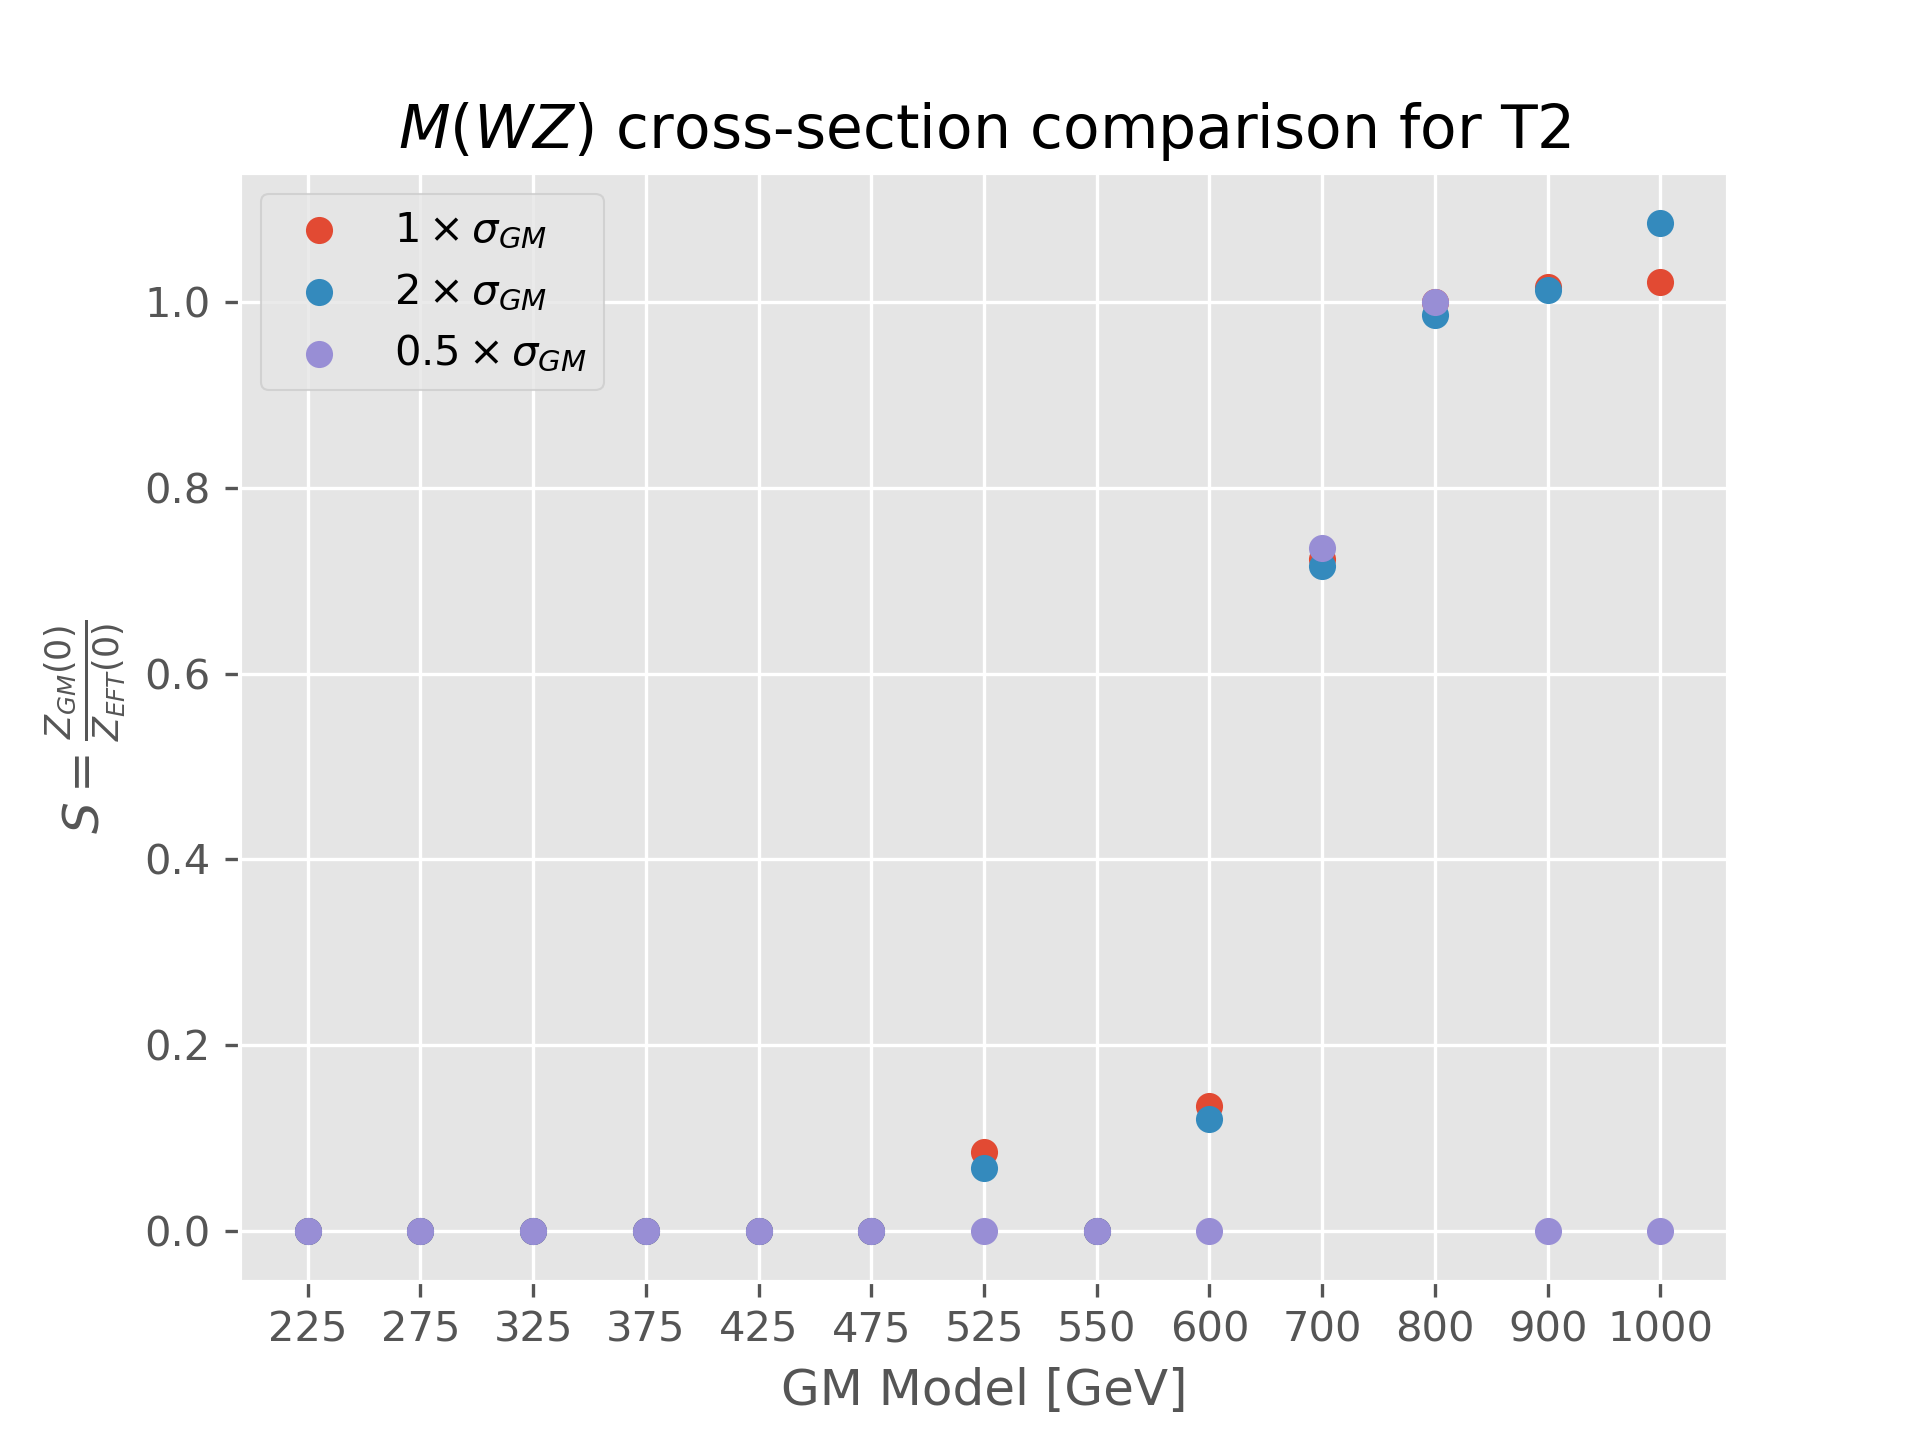
\includegraphics[width=\textwidth]{Plots/gm_relevanze/MWZ_comparision_T2.png}

    \end{subfigure}

\end{figure}


\begin{figure}[h]
    \centering
    \begin{subfigure}{0.45\textwidth}
        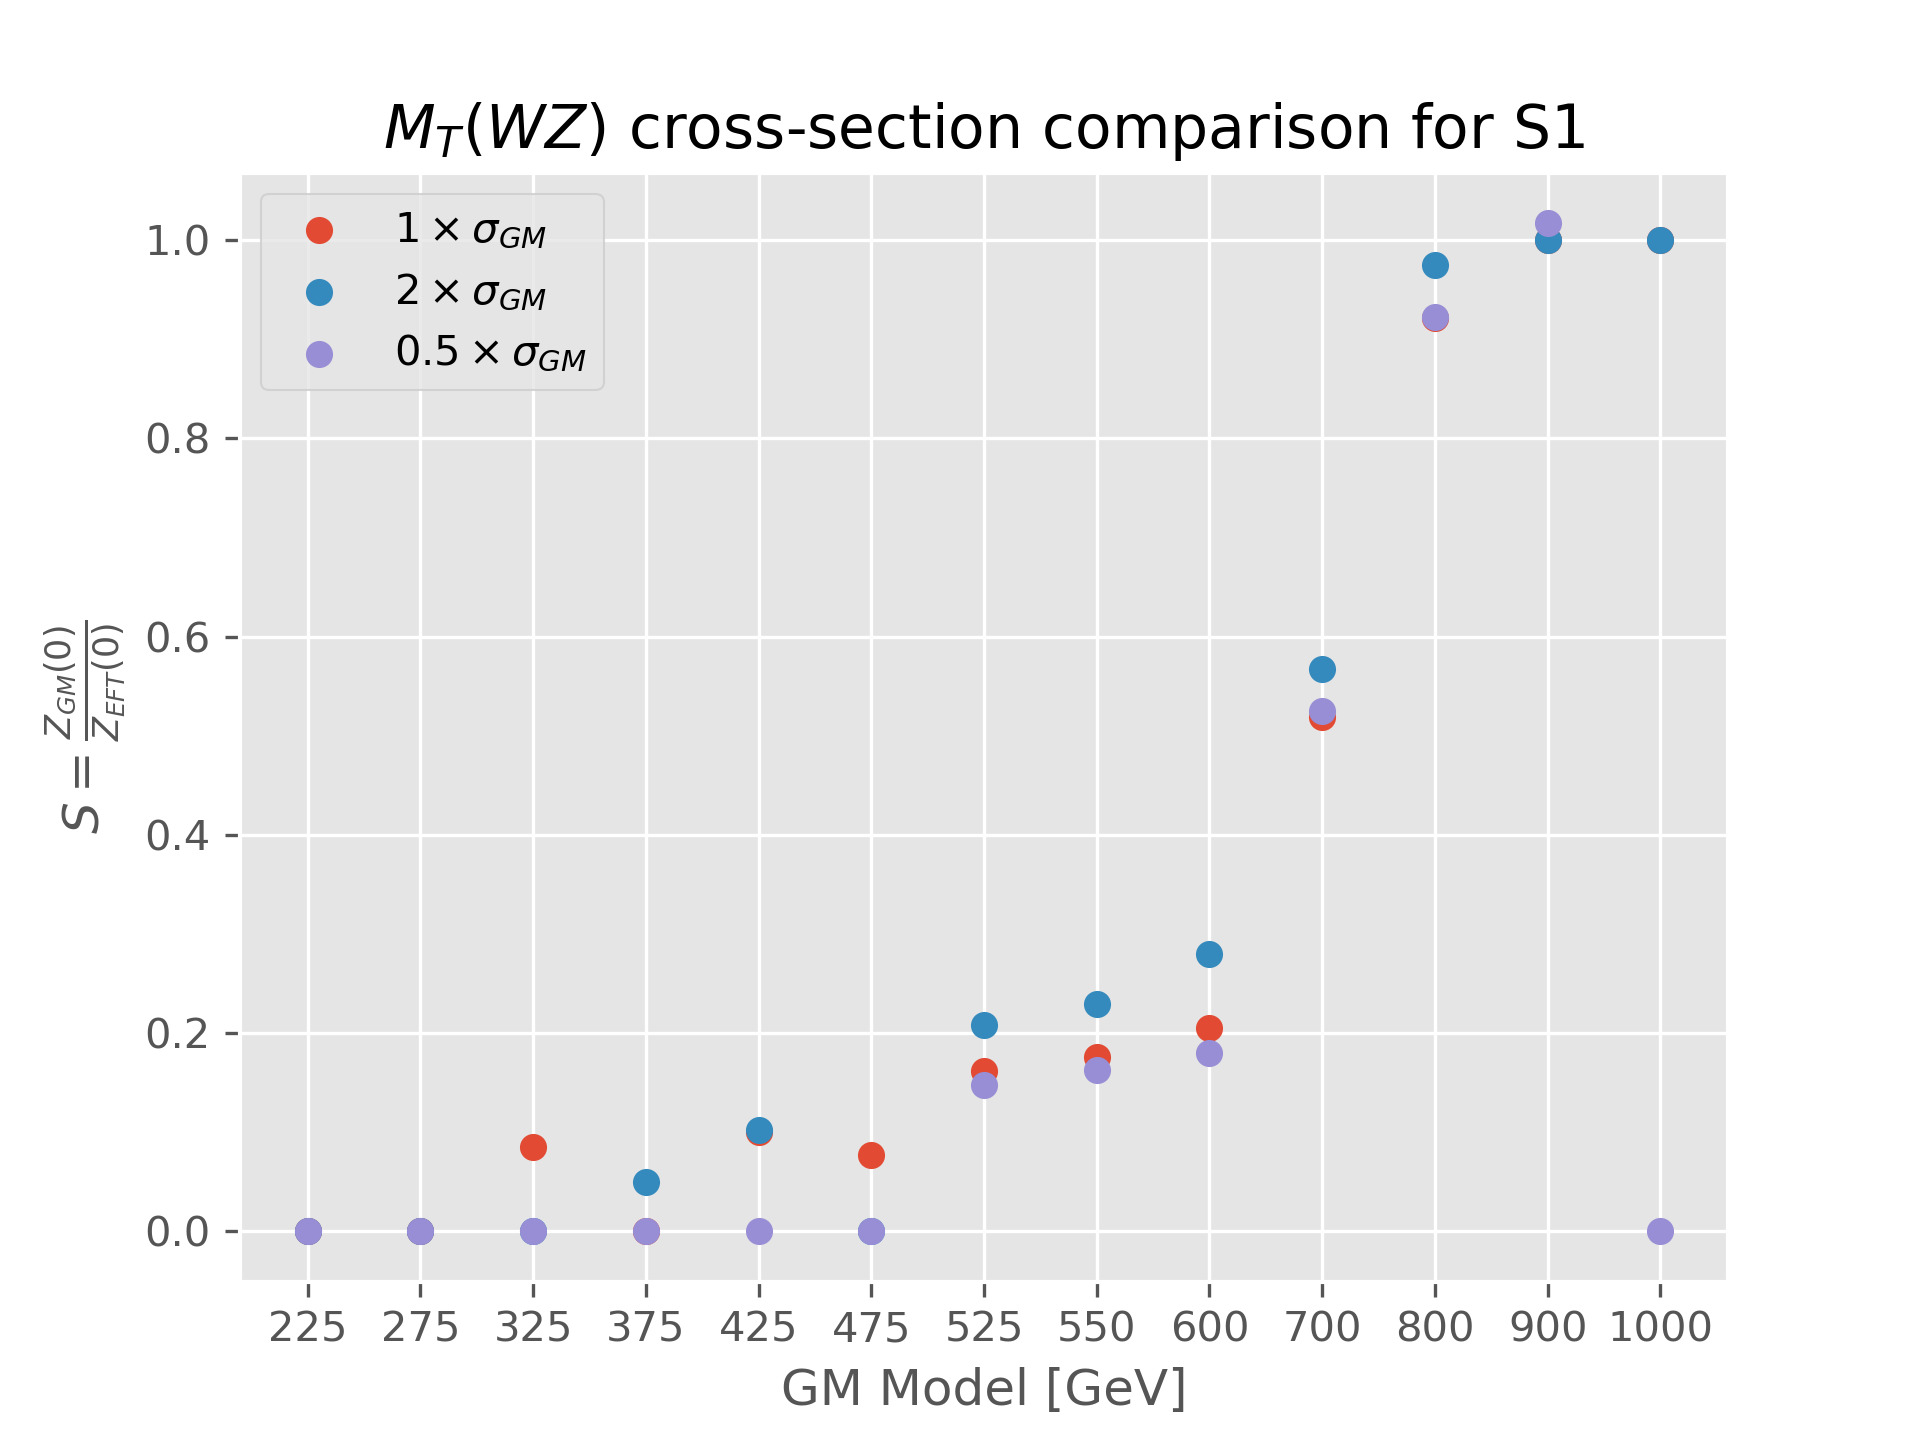
\includegraphics[width=\textwidth]{Plots/gm_relevanze/MTWZ_comparision_S1.png}

    \end{subfigure}
    \begin{subfigure}{0.45\textwidth}
        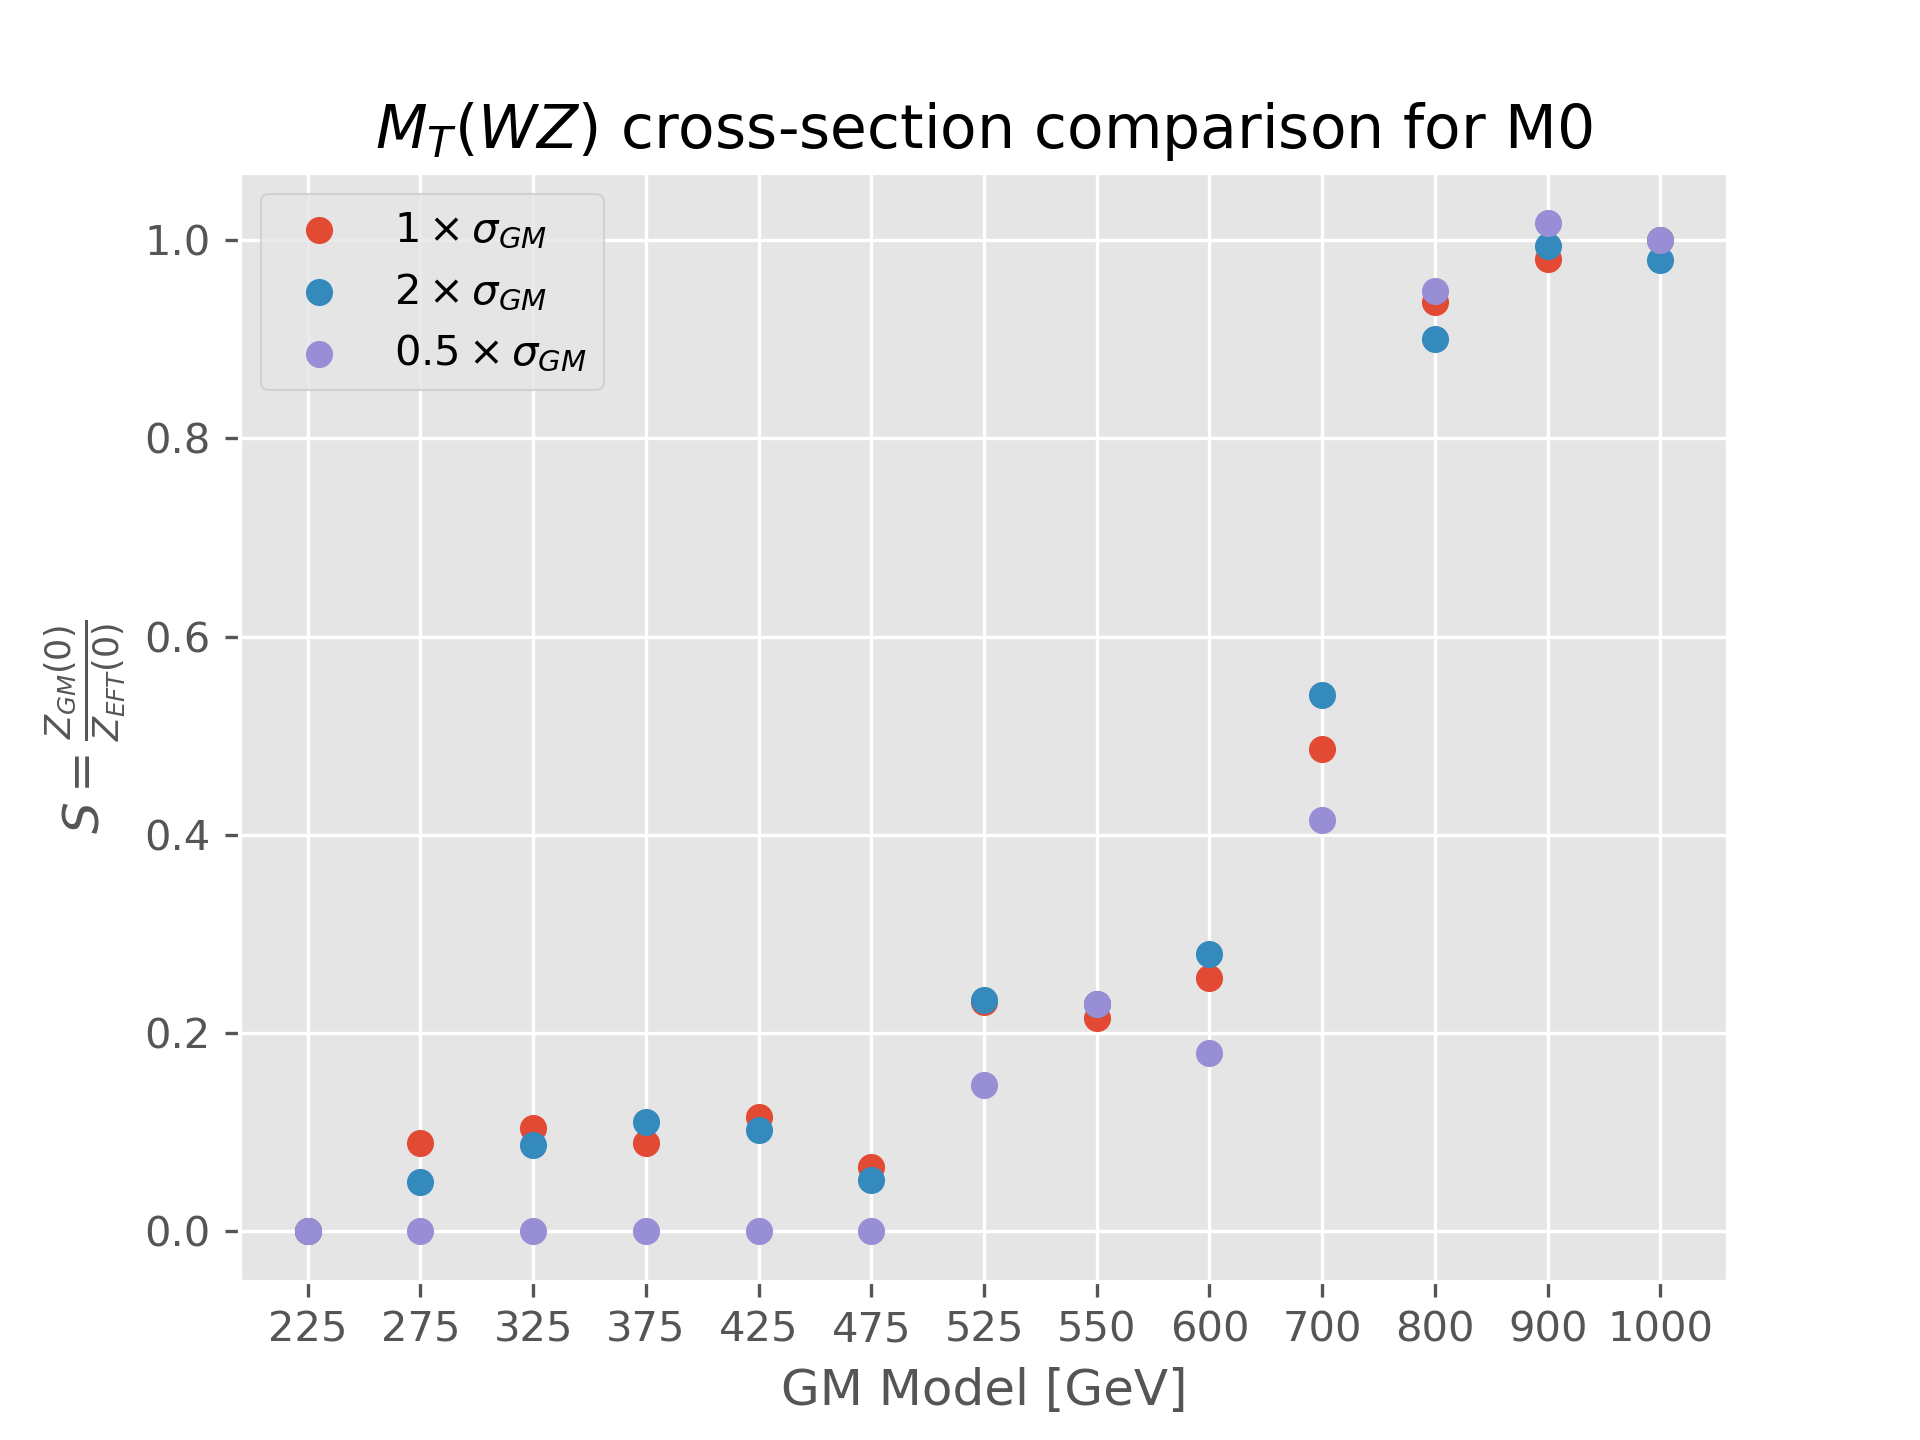
\includegraphics[width=\textwidth]{Plots/gm_relevanze/MTWZ_comparision_M0.png}

    \end{subfigure}
    \begin{subfigure}{0.45\textwidth}
        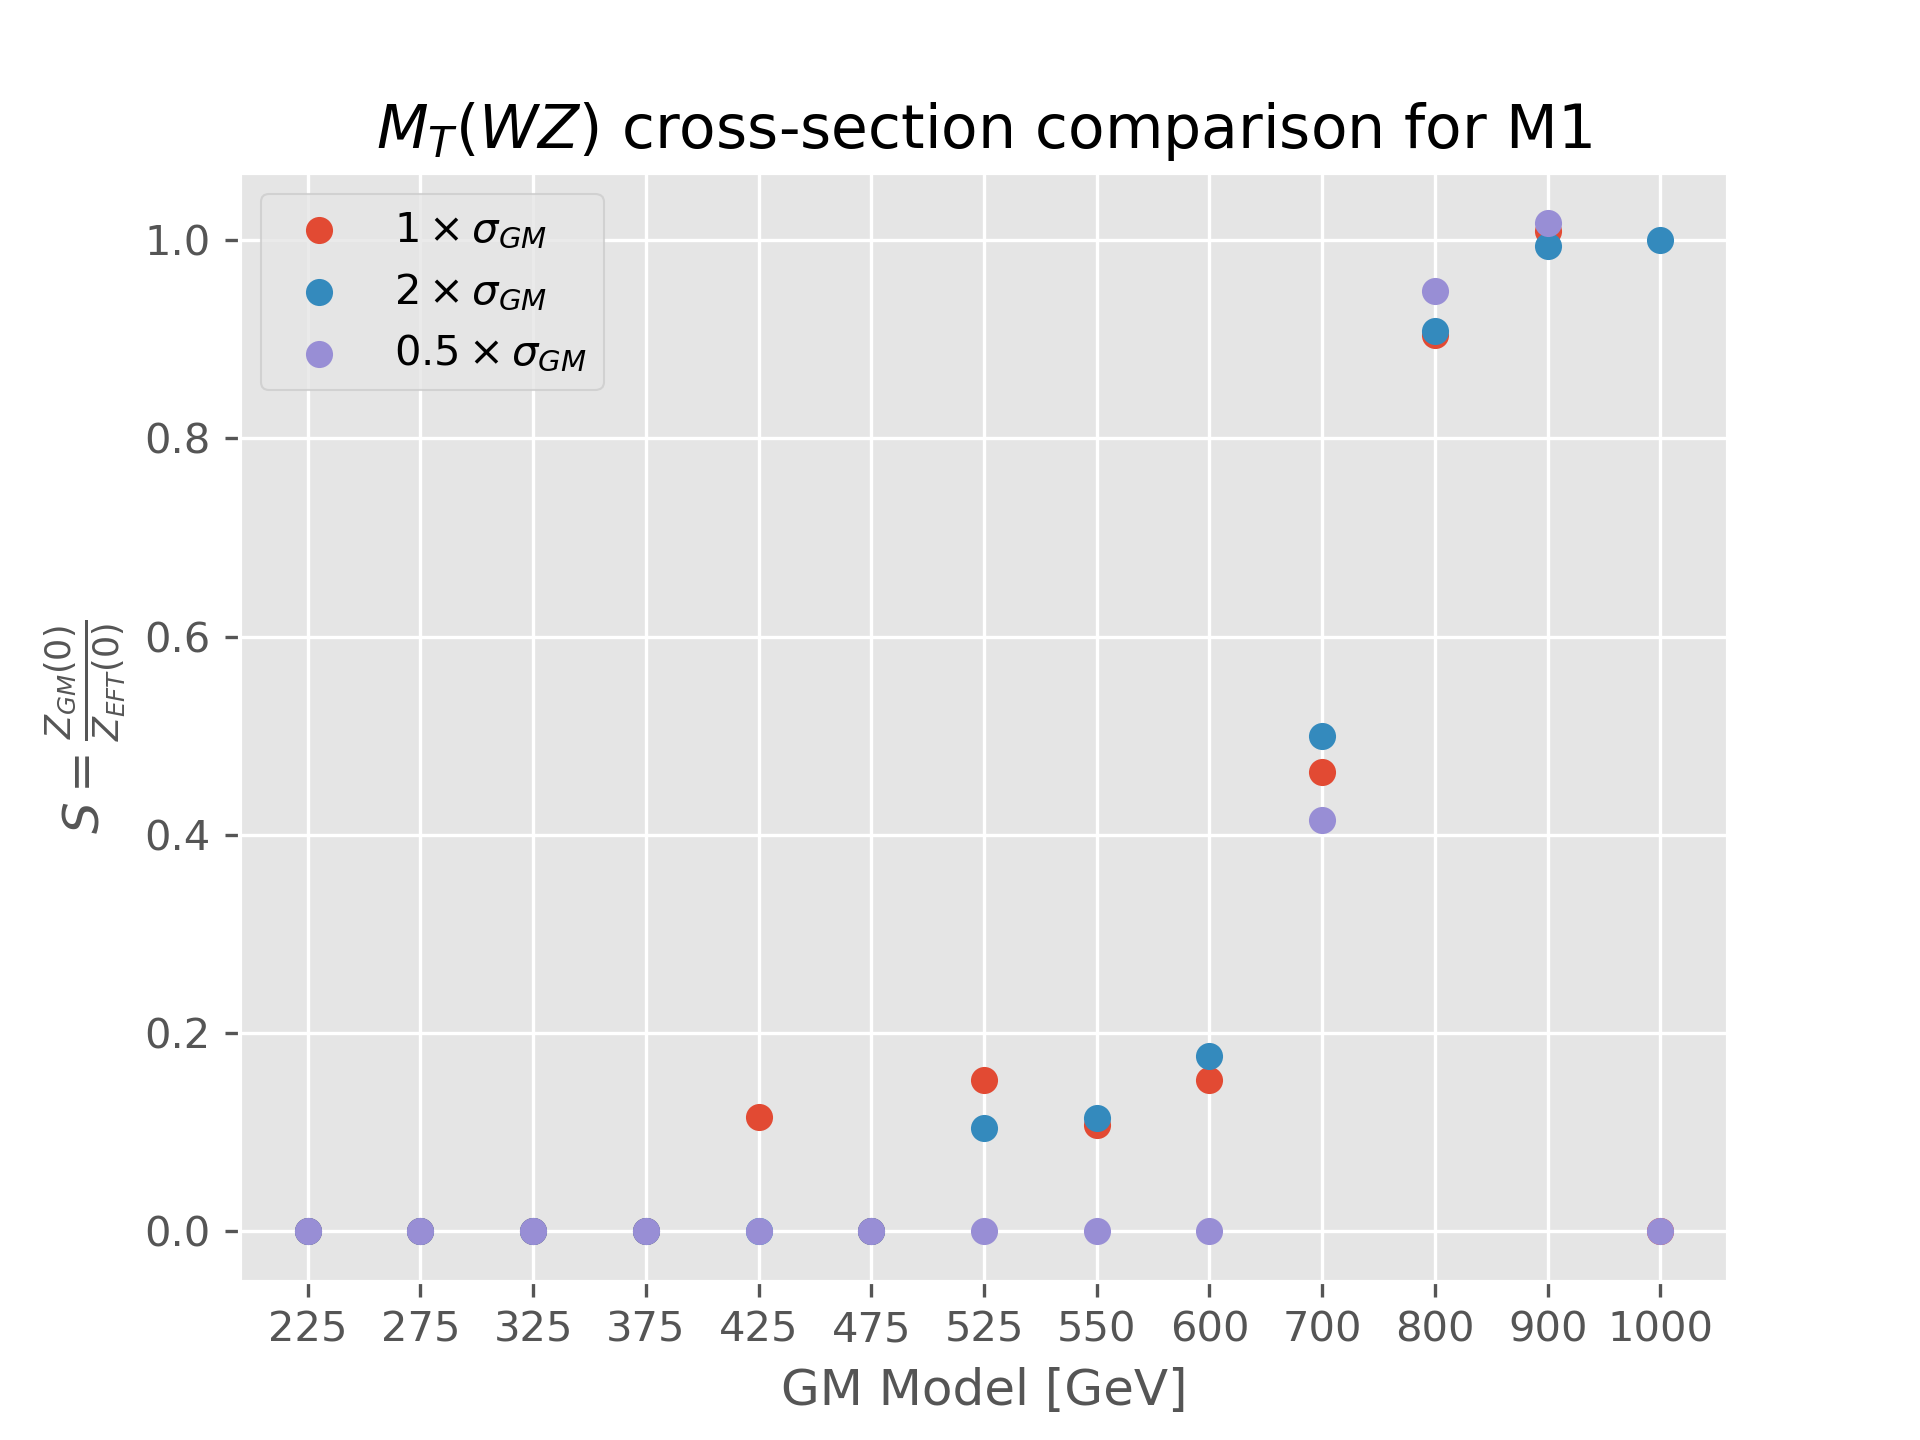
\includegraphics[width=\textwidth]{Plots/gm_relevanze/MTWZ_comparision_M1.png}

    \end{subfigure}
    \begin{subfigure}{0.45\textwidth}
        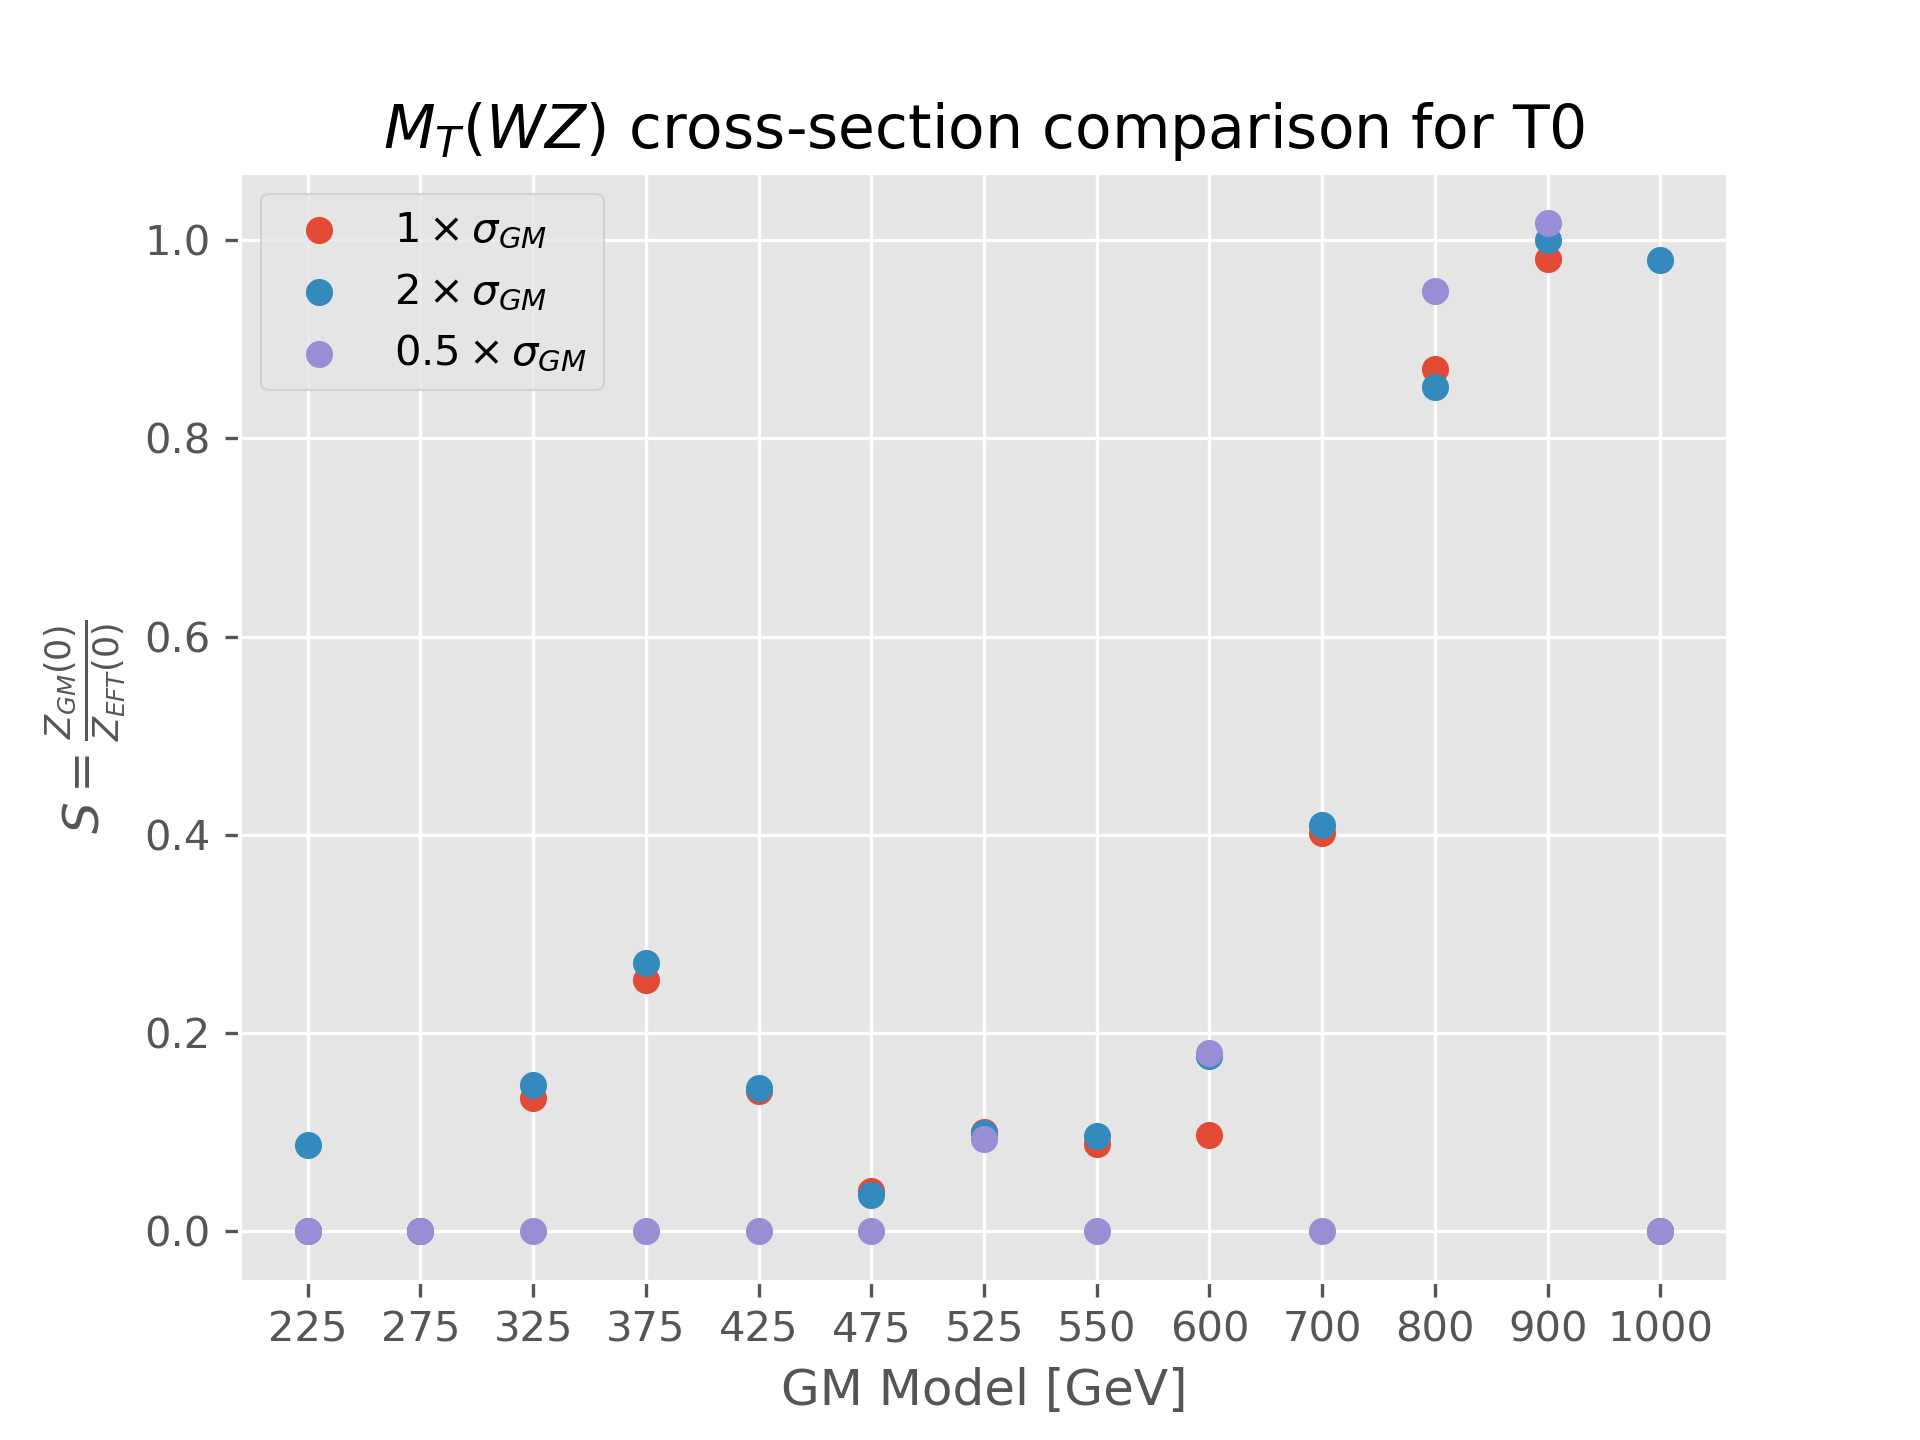
\includegraphics[width=\textwidth]{Plots/gm_relevanze/MTWZ_comparision_T0.png}

    \end{subfigure}
    \begin{subfigure}{0.45\textwidth}
        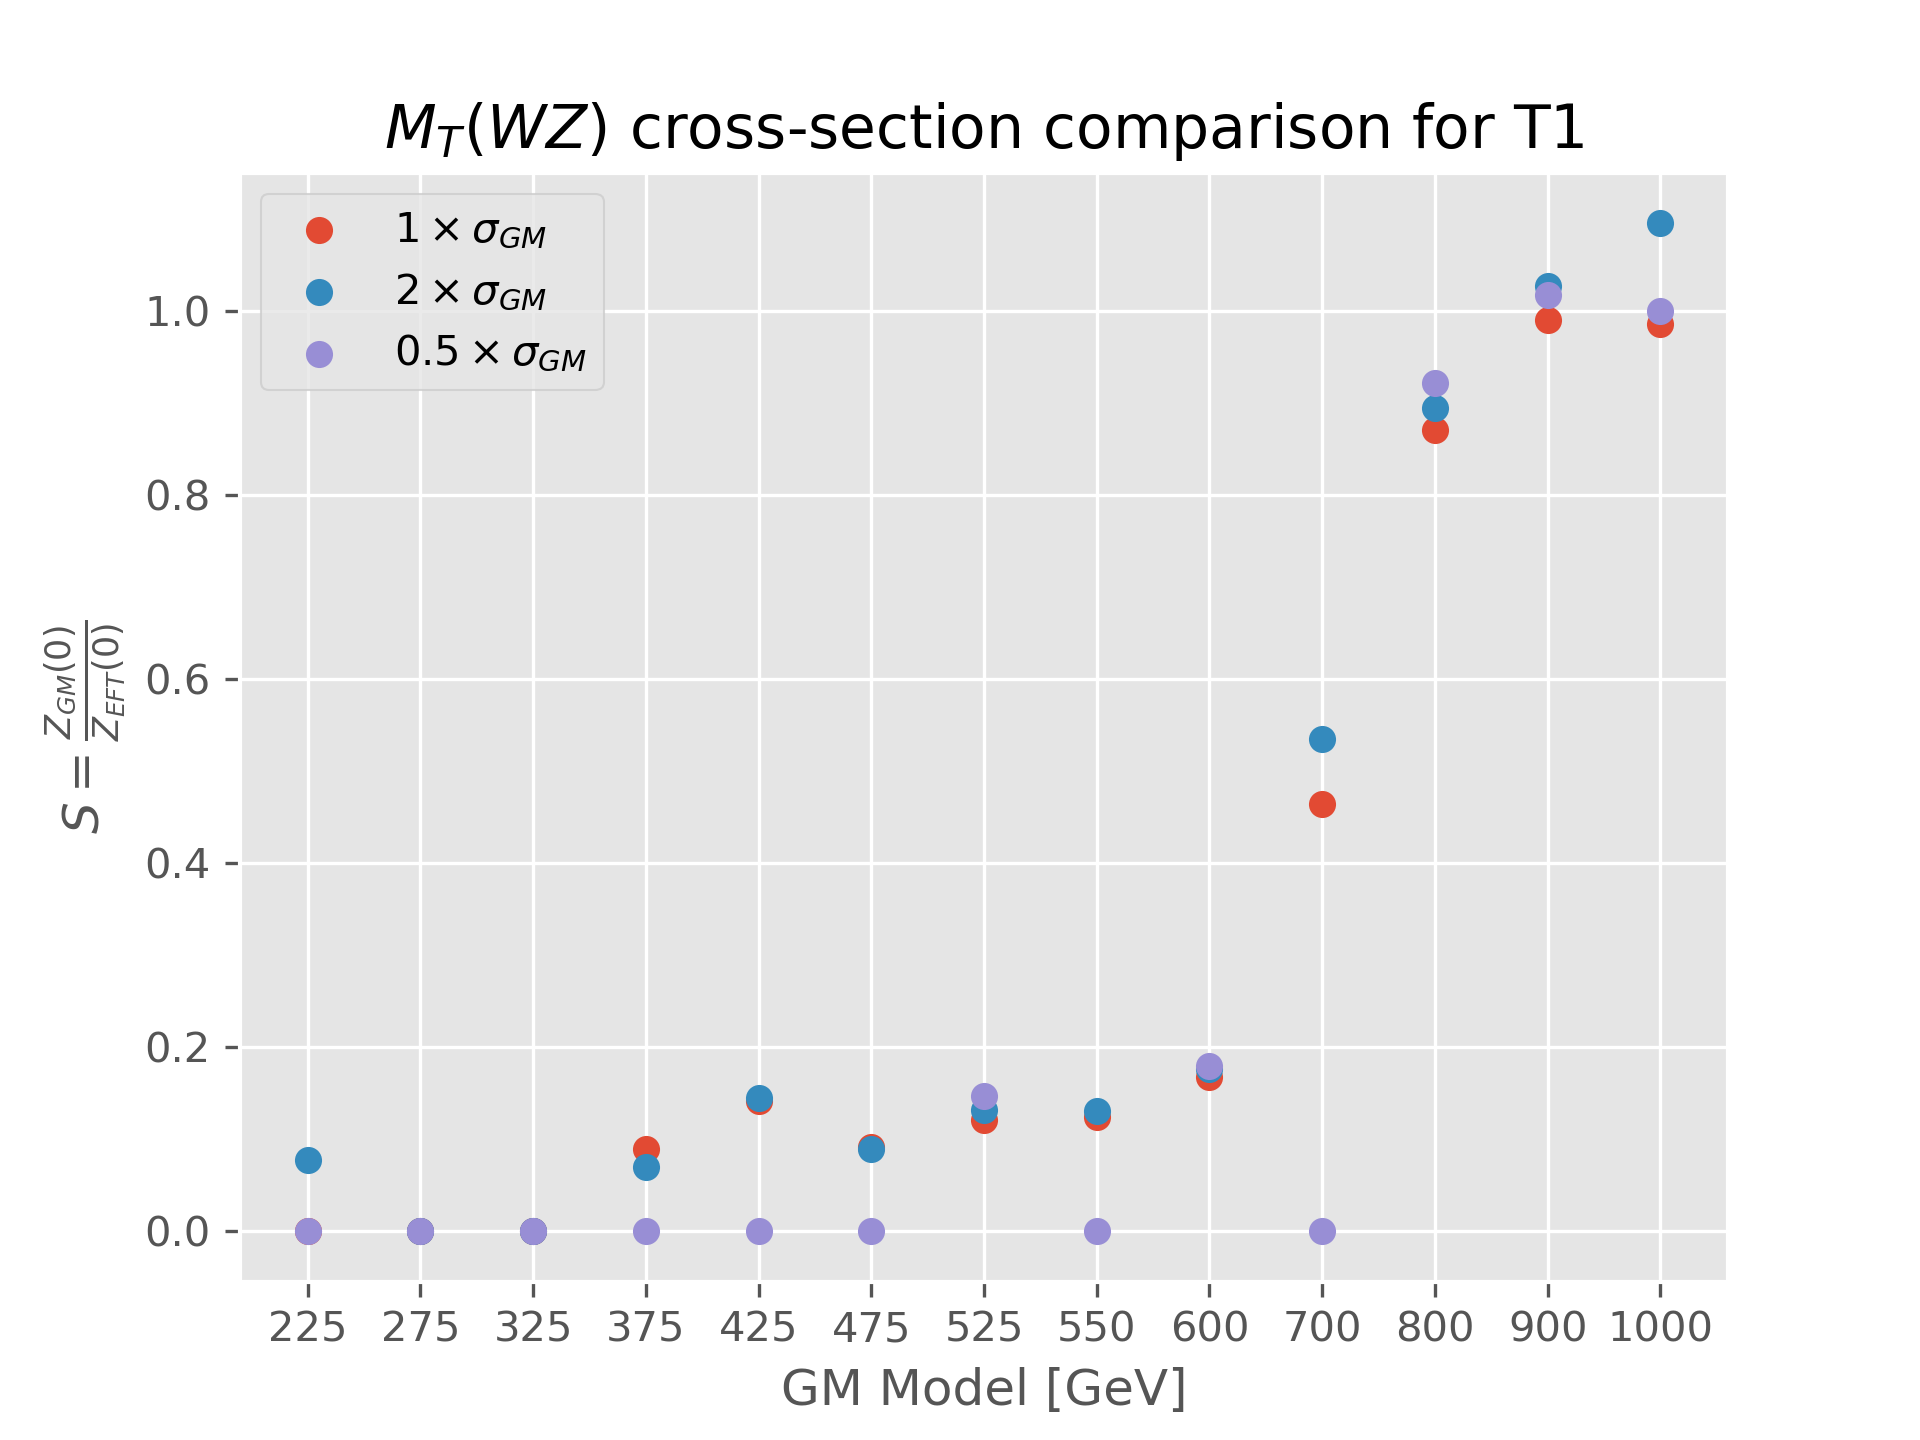
\includegraphics[width=\textwidth]{Plots/gm_relevanze/MTWZ_comparision_T1.png}

    \end{subfigure}
    \begin{subfigure}{0.45\textwidth}
        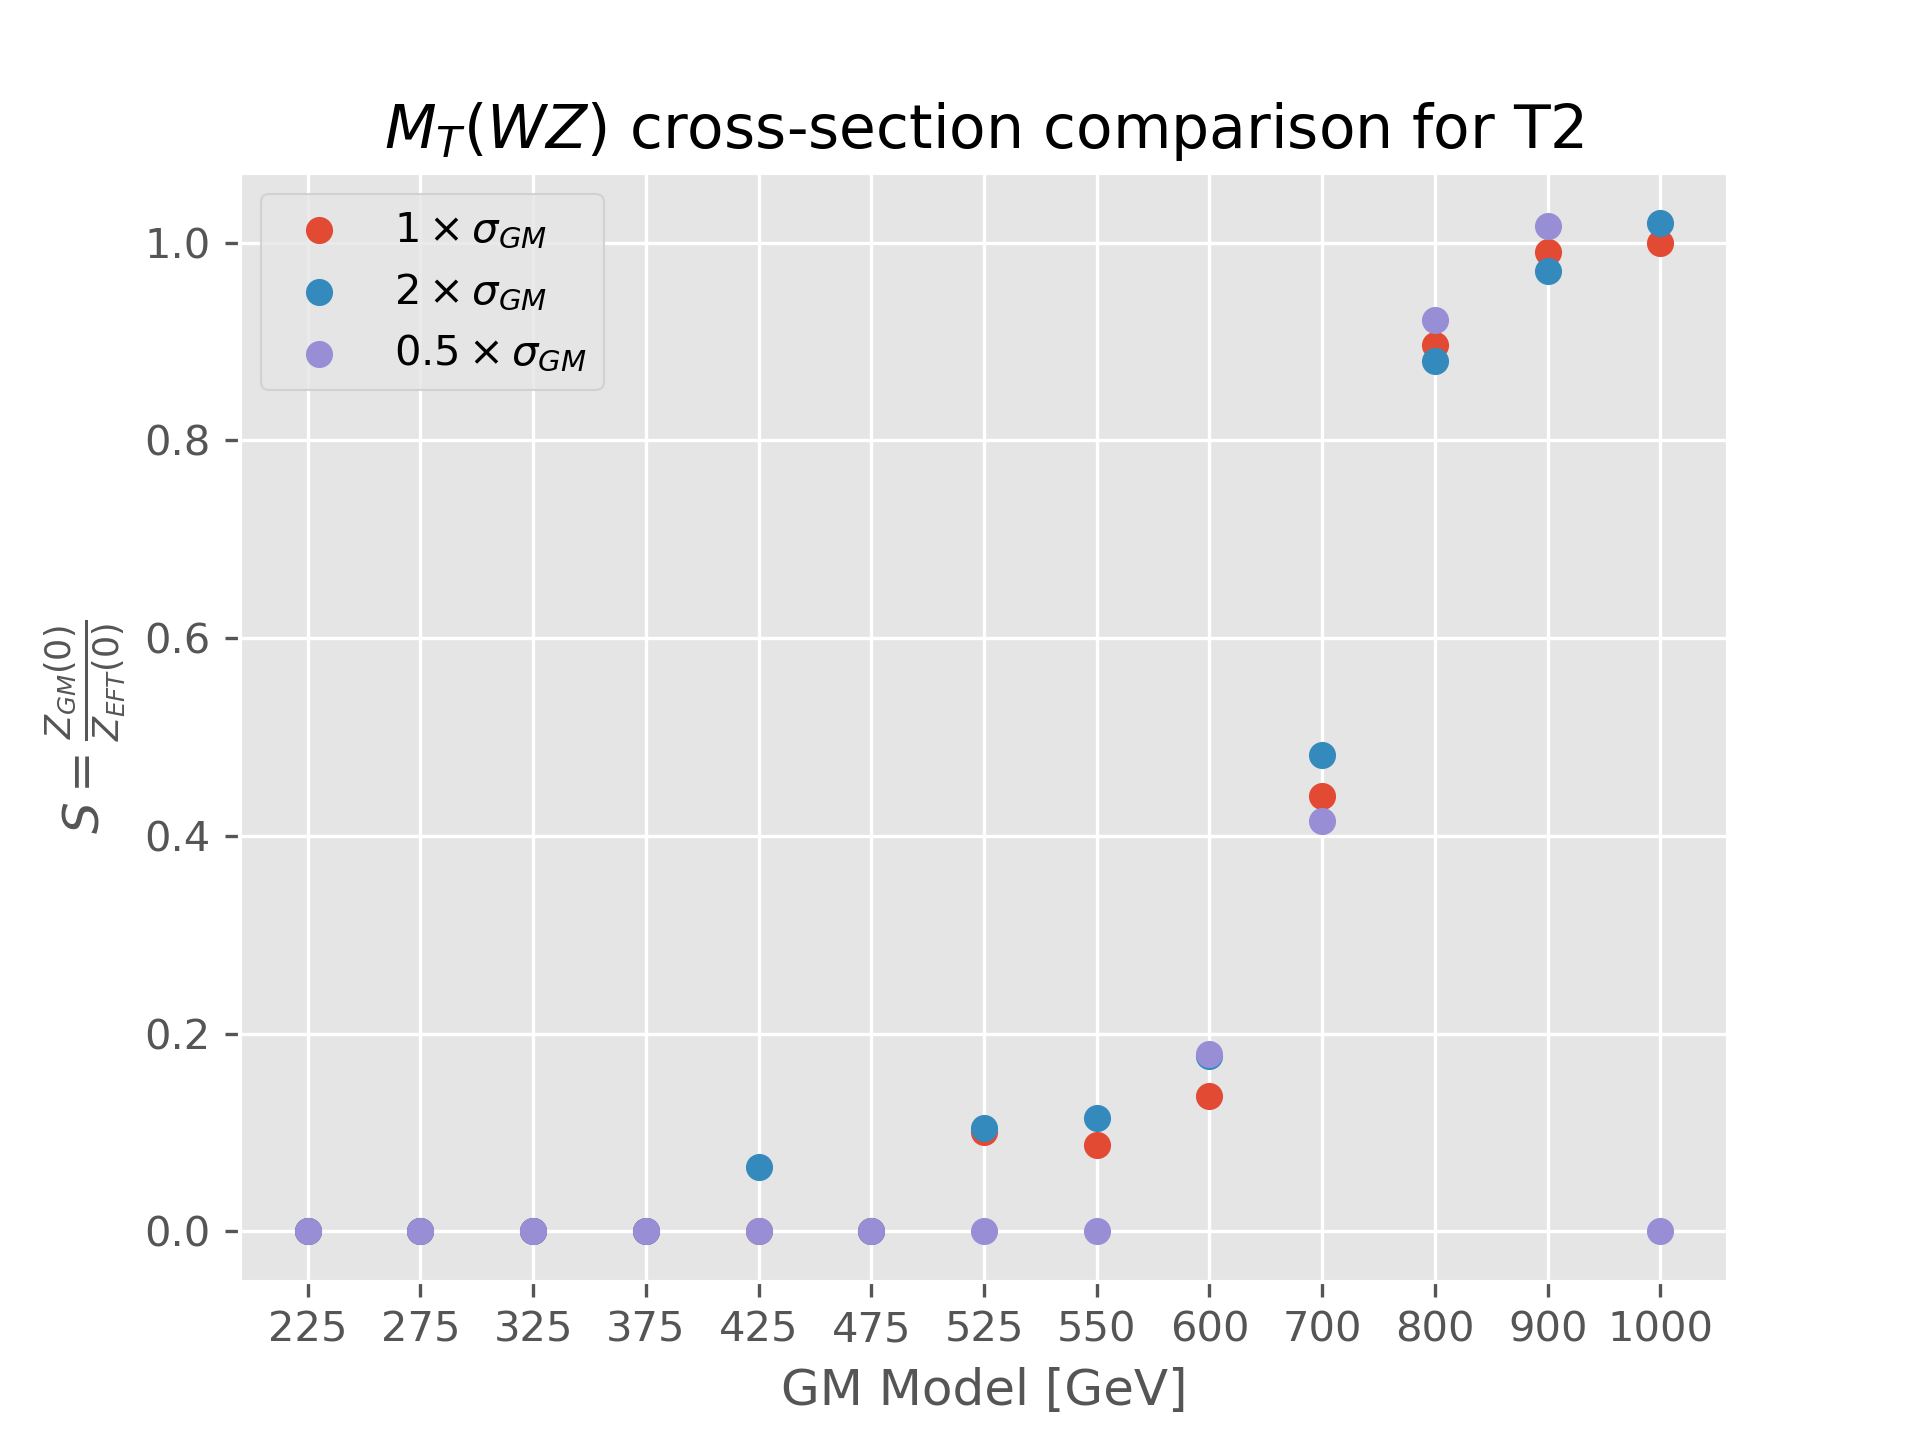
\includegraphics[width=\textwidth]{Plots/gm_relevanze/MTWZ_comparision_T2.png}

    \end{subfigure}

\end{figure}

\section{Resonances}
\label{sec:further_resonace}
\subsection{900 GeV resonance}
\begin{figure}[h]

    \centering
    \begin{subfigure}{0.45\textwidth}
        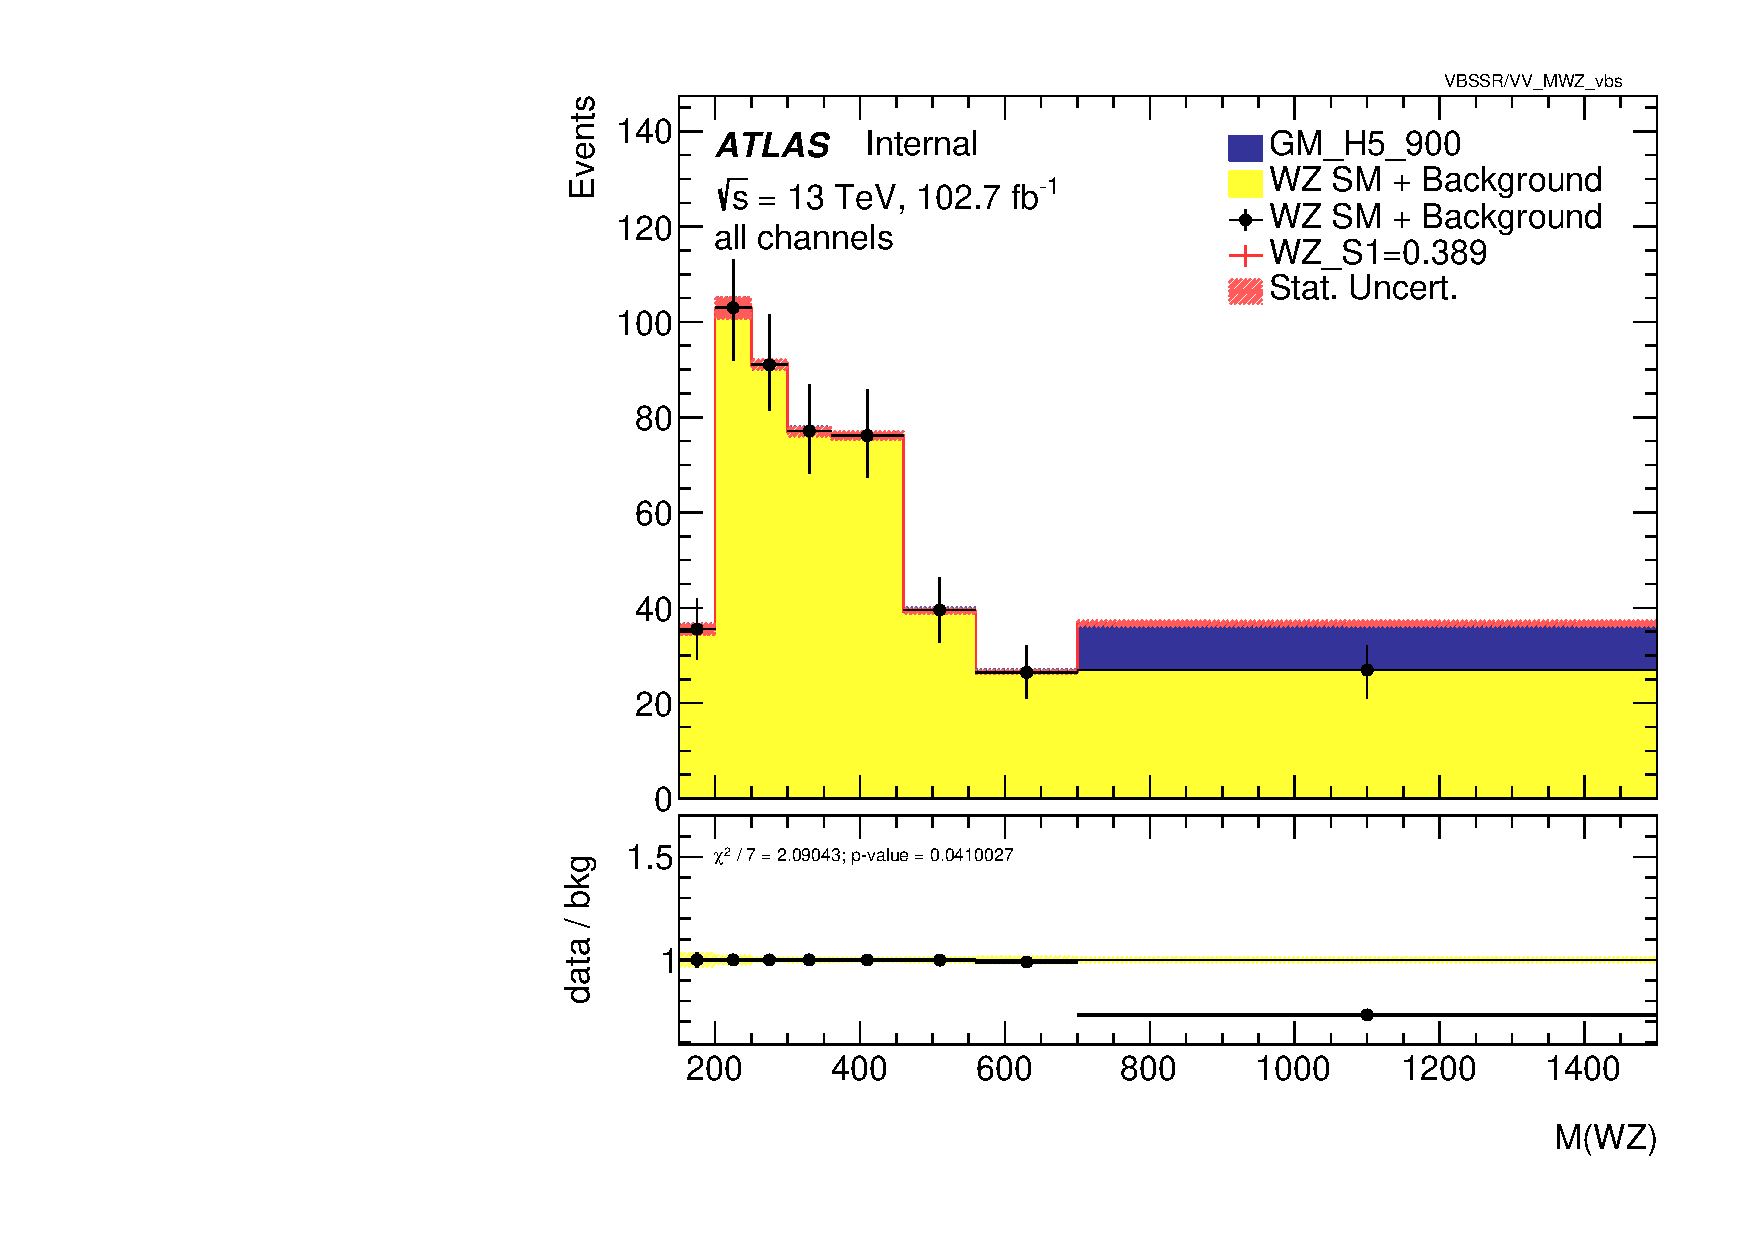
\includegraphics[width=\textwidth]{Plots/ALL_MWZ_right_color/GM_H5_900/S1/2022-05-07/VBSSR/all_VV_MWZ_vbs.pdf}
    \end{subfigure}
    \begin{subfigure}{0.45\textwidth}
        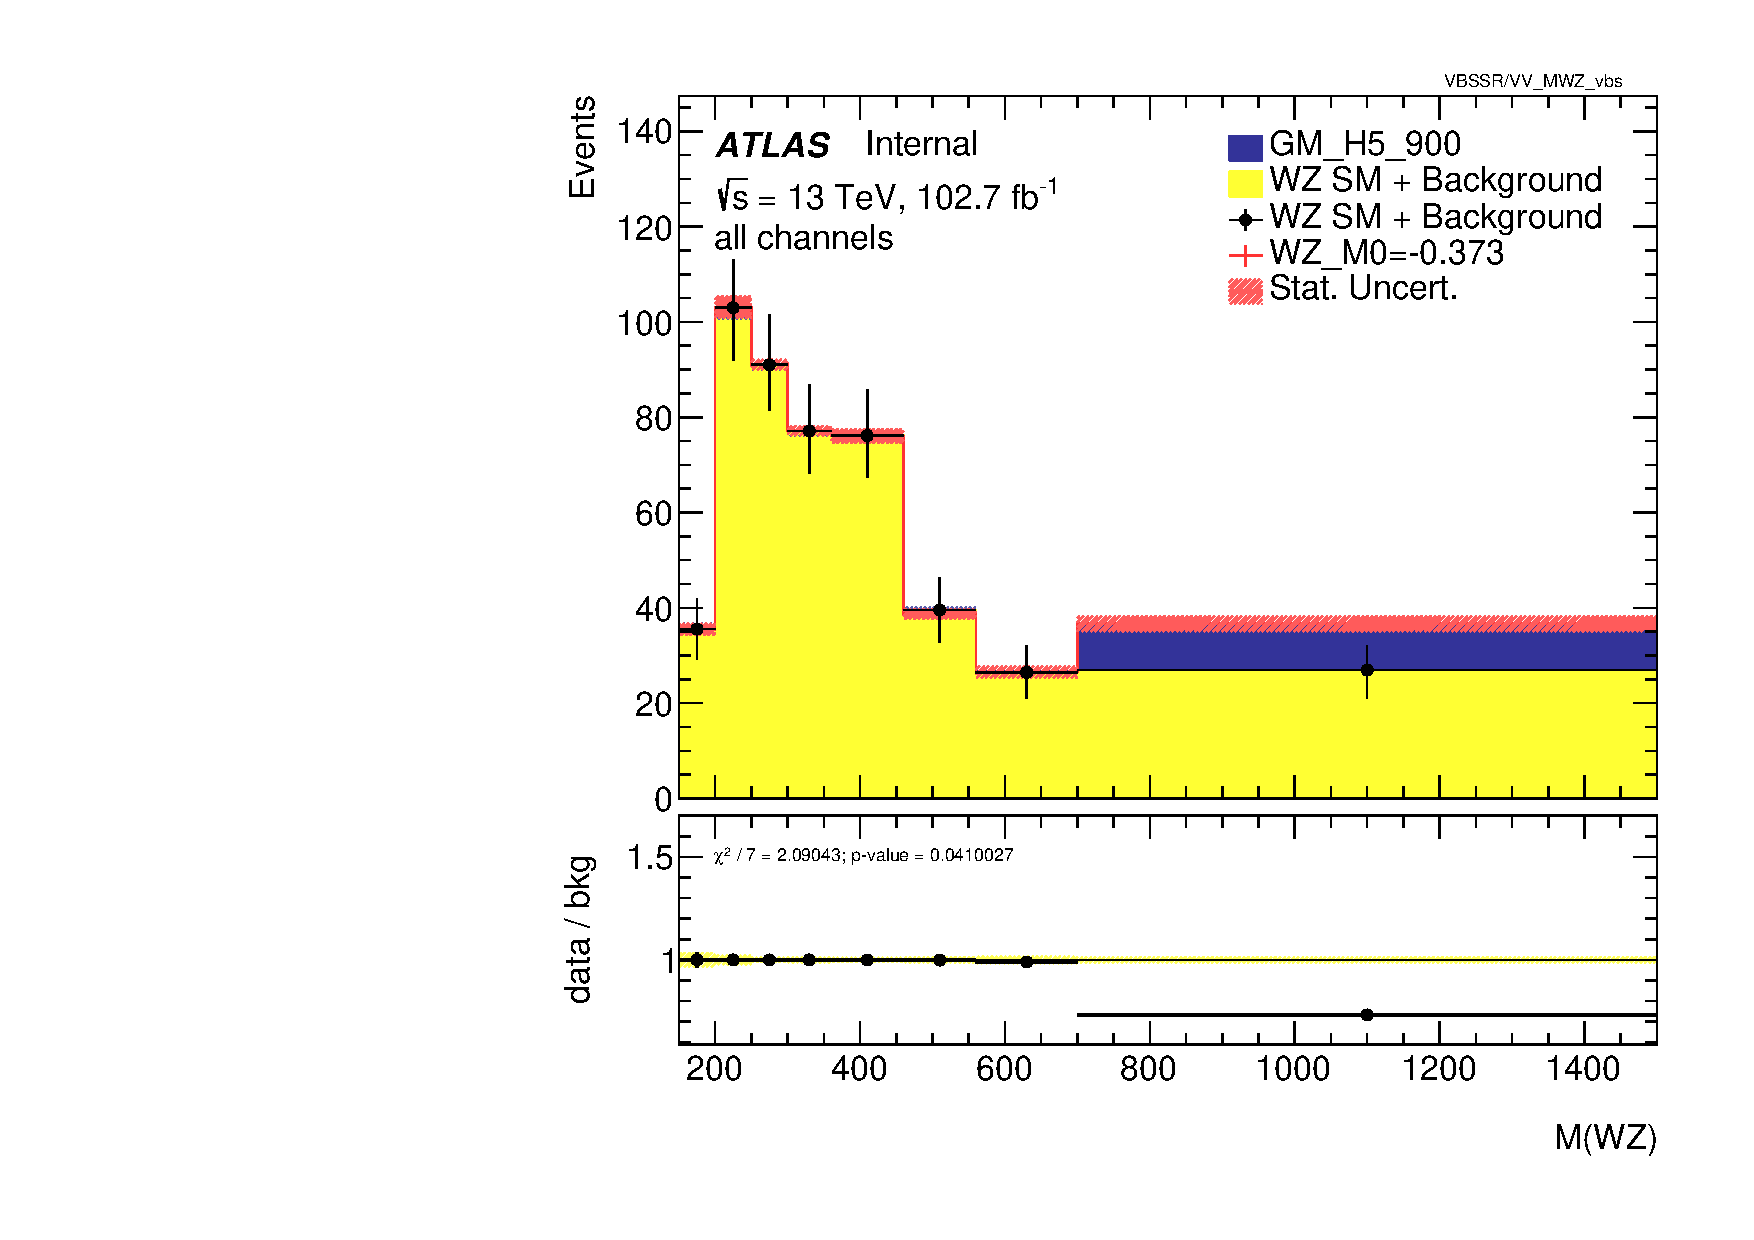
\includegraphics[width=\textwidth]{Plots/ALL_MWZ_right_color/GM_H5_900/M0/2022-05-07/VBSSR/all_VV_MWZ_vbs.pdf}
    \end{subfigure}
    \begin{subfigure}{0.45\textwidth}
        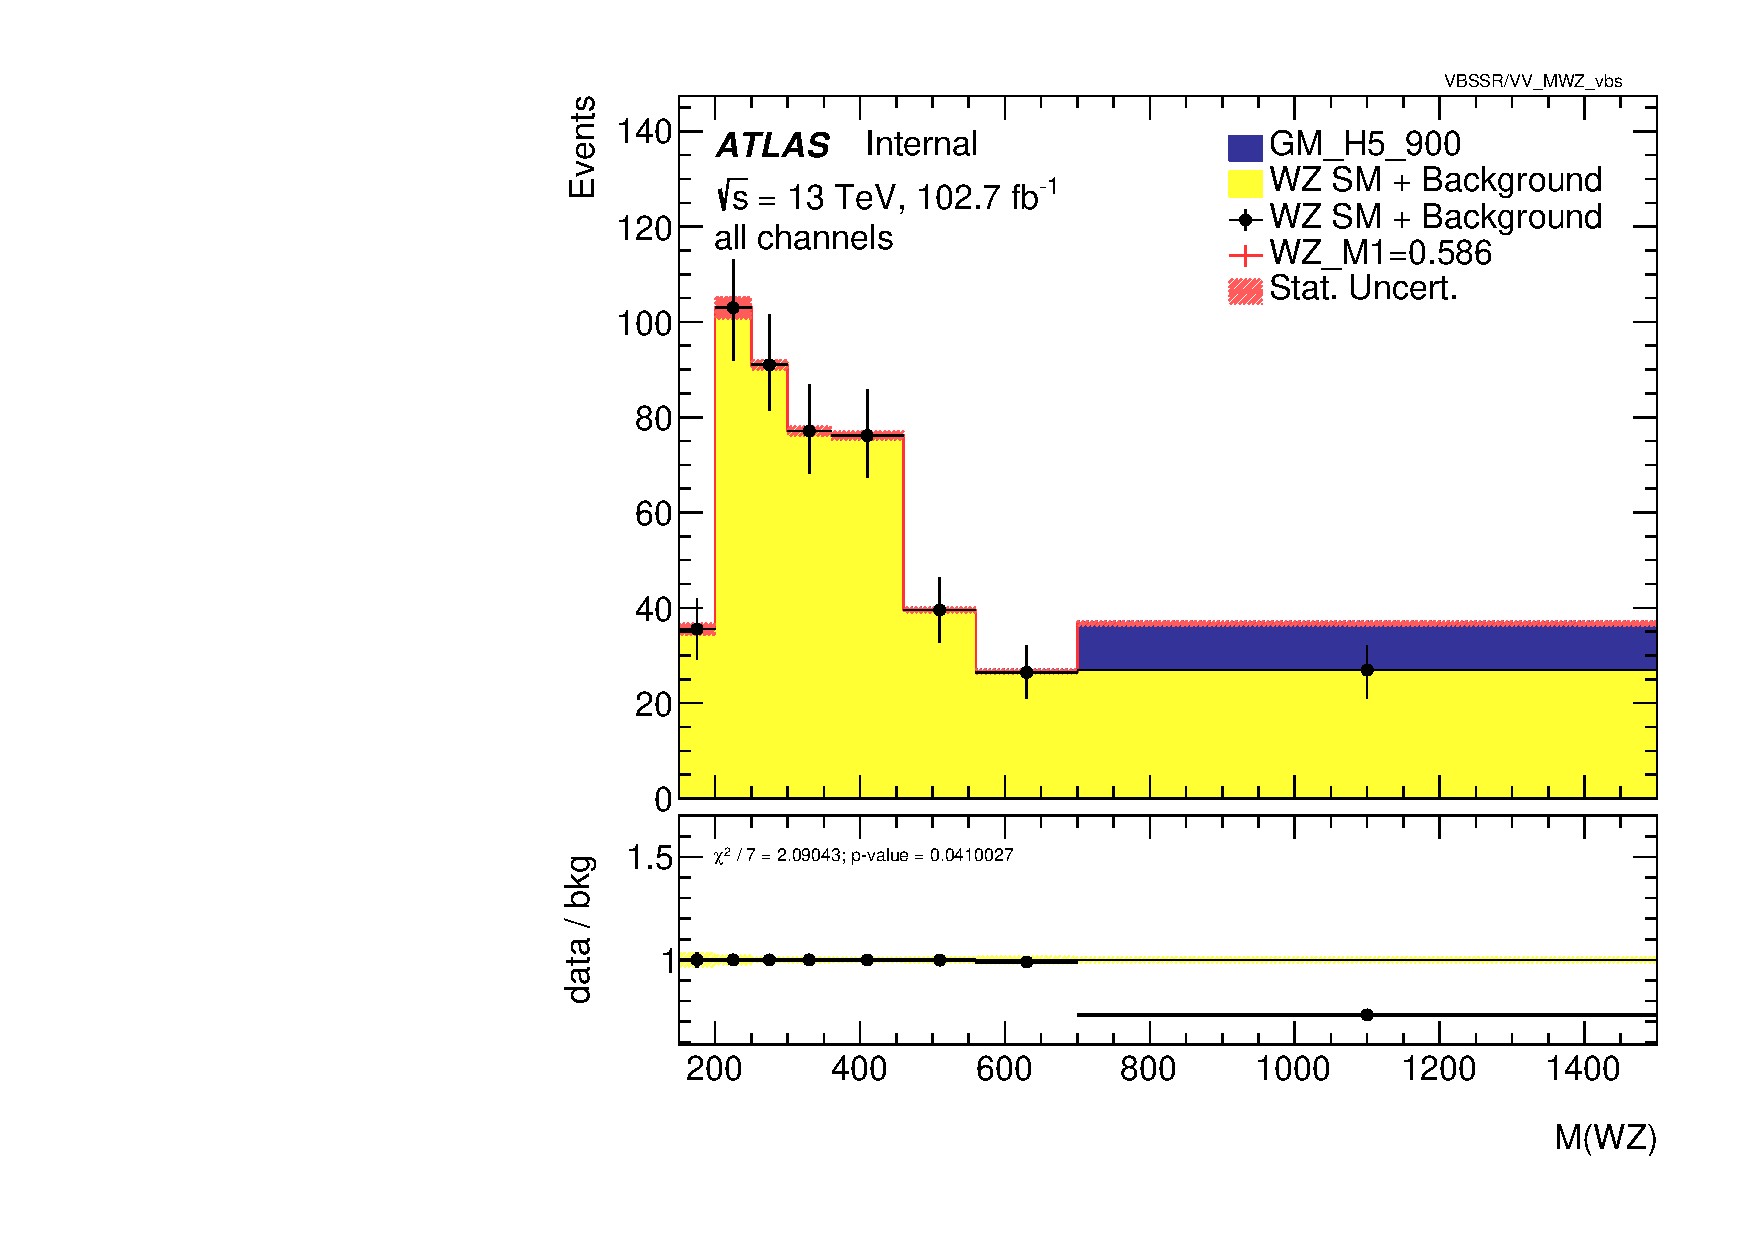
\includegraphics[width=\textwidth]{Plots/ALL_MWZ_right_color/GM_H5_900/M1/2022-05-07/VBSSR/all_VV_MWZ_vbs.pdf}
    \end{subfigure}
    \begin{subfigure}{0.45\textwidth}
        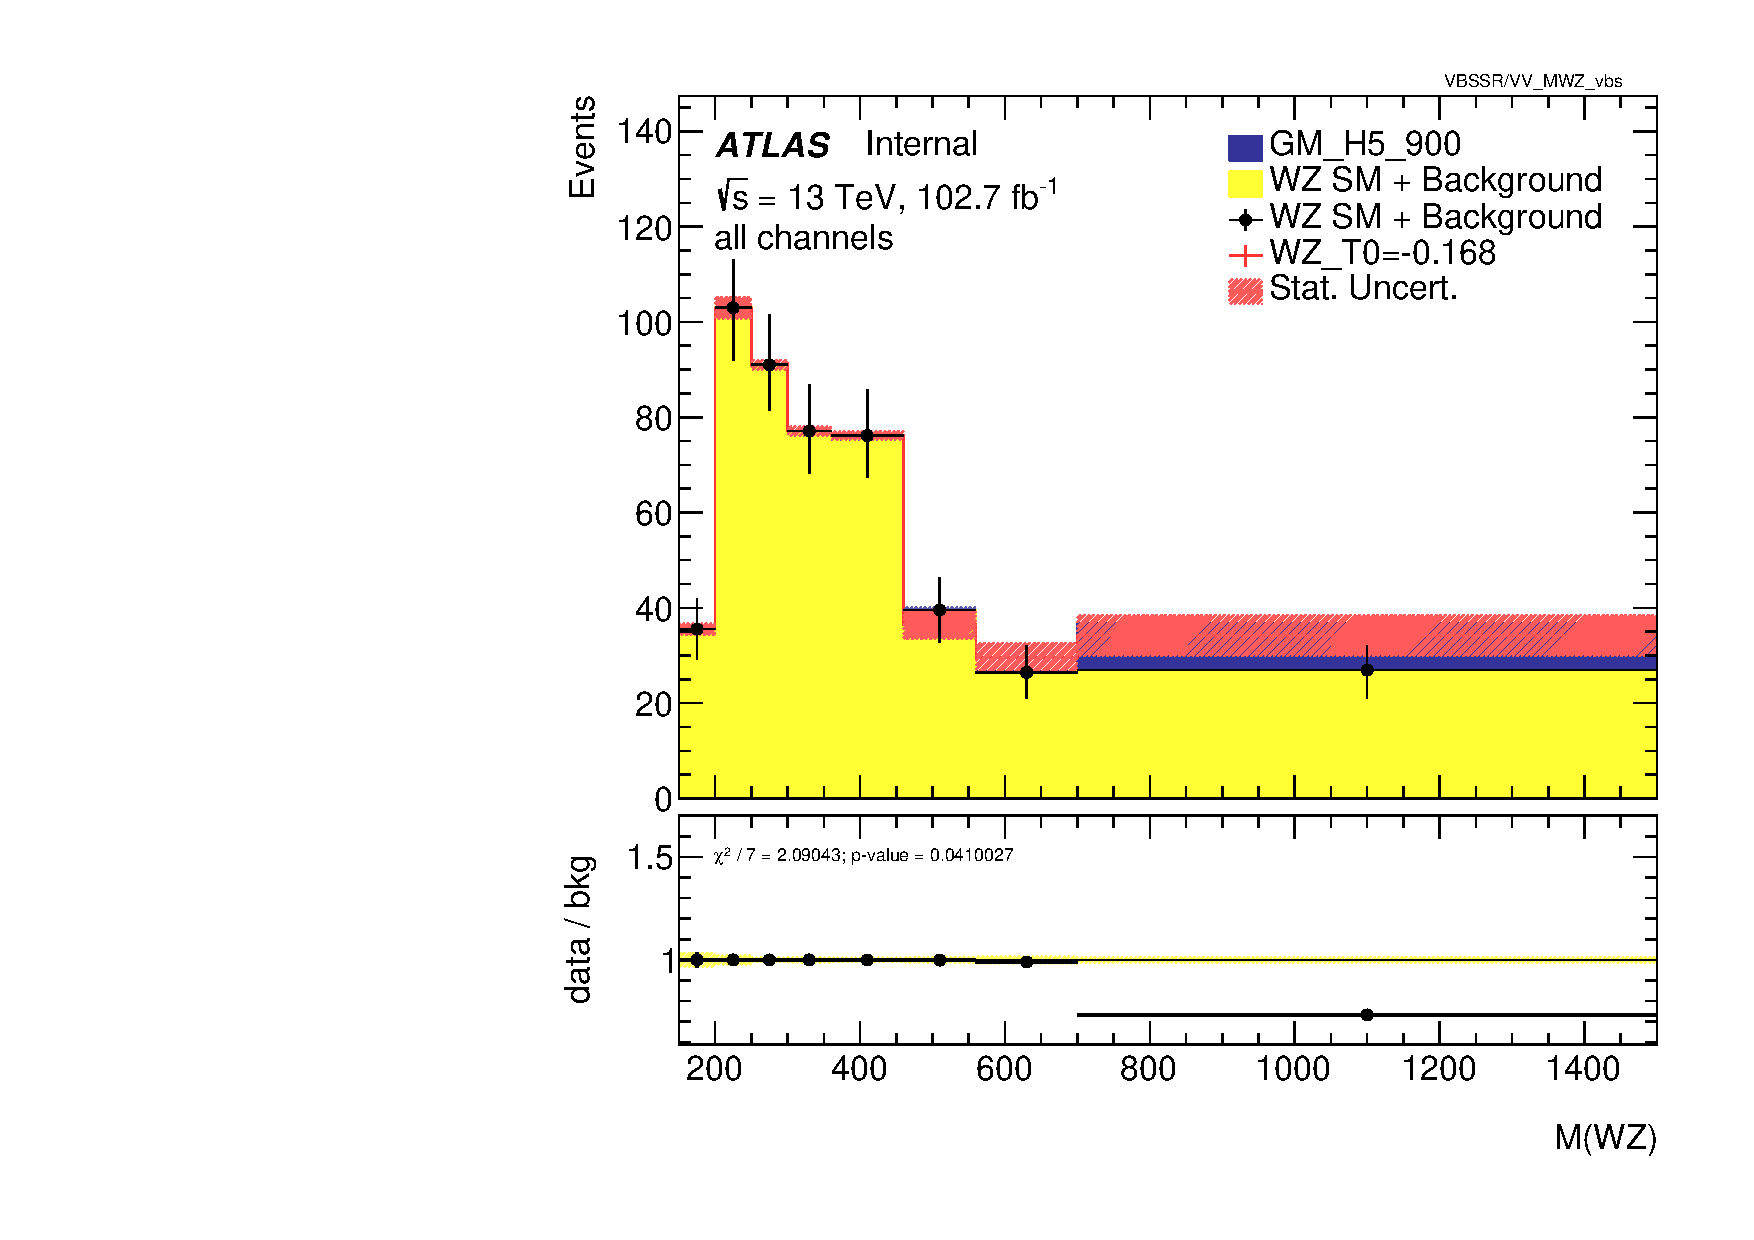
\includegraphics[width=\textwidth]{Plots/ALL_MWZ_right_color/GM_H5_900/T0/2022-05-07/VBSSR/all_VV_MWZ_vbs.pdf}
    \end{subfigure}
    \begin{subfigure}{0.45\textwidth}
        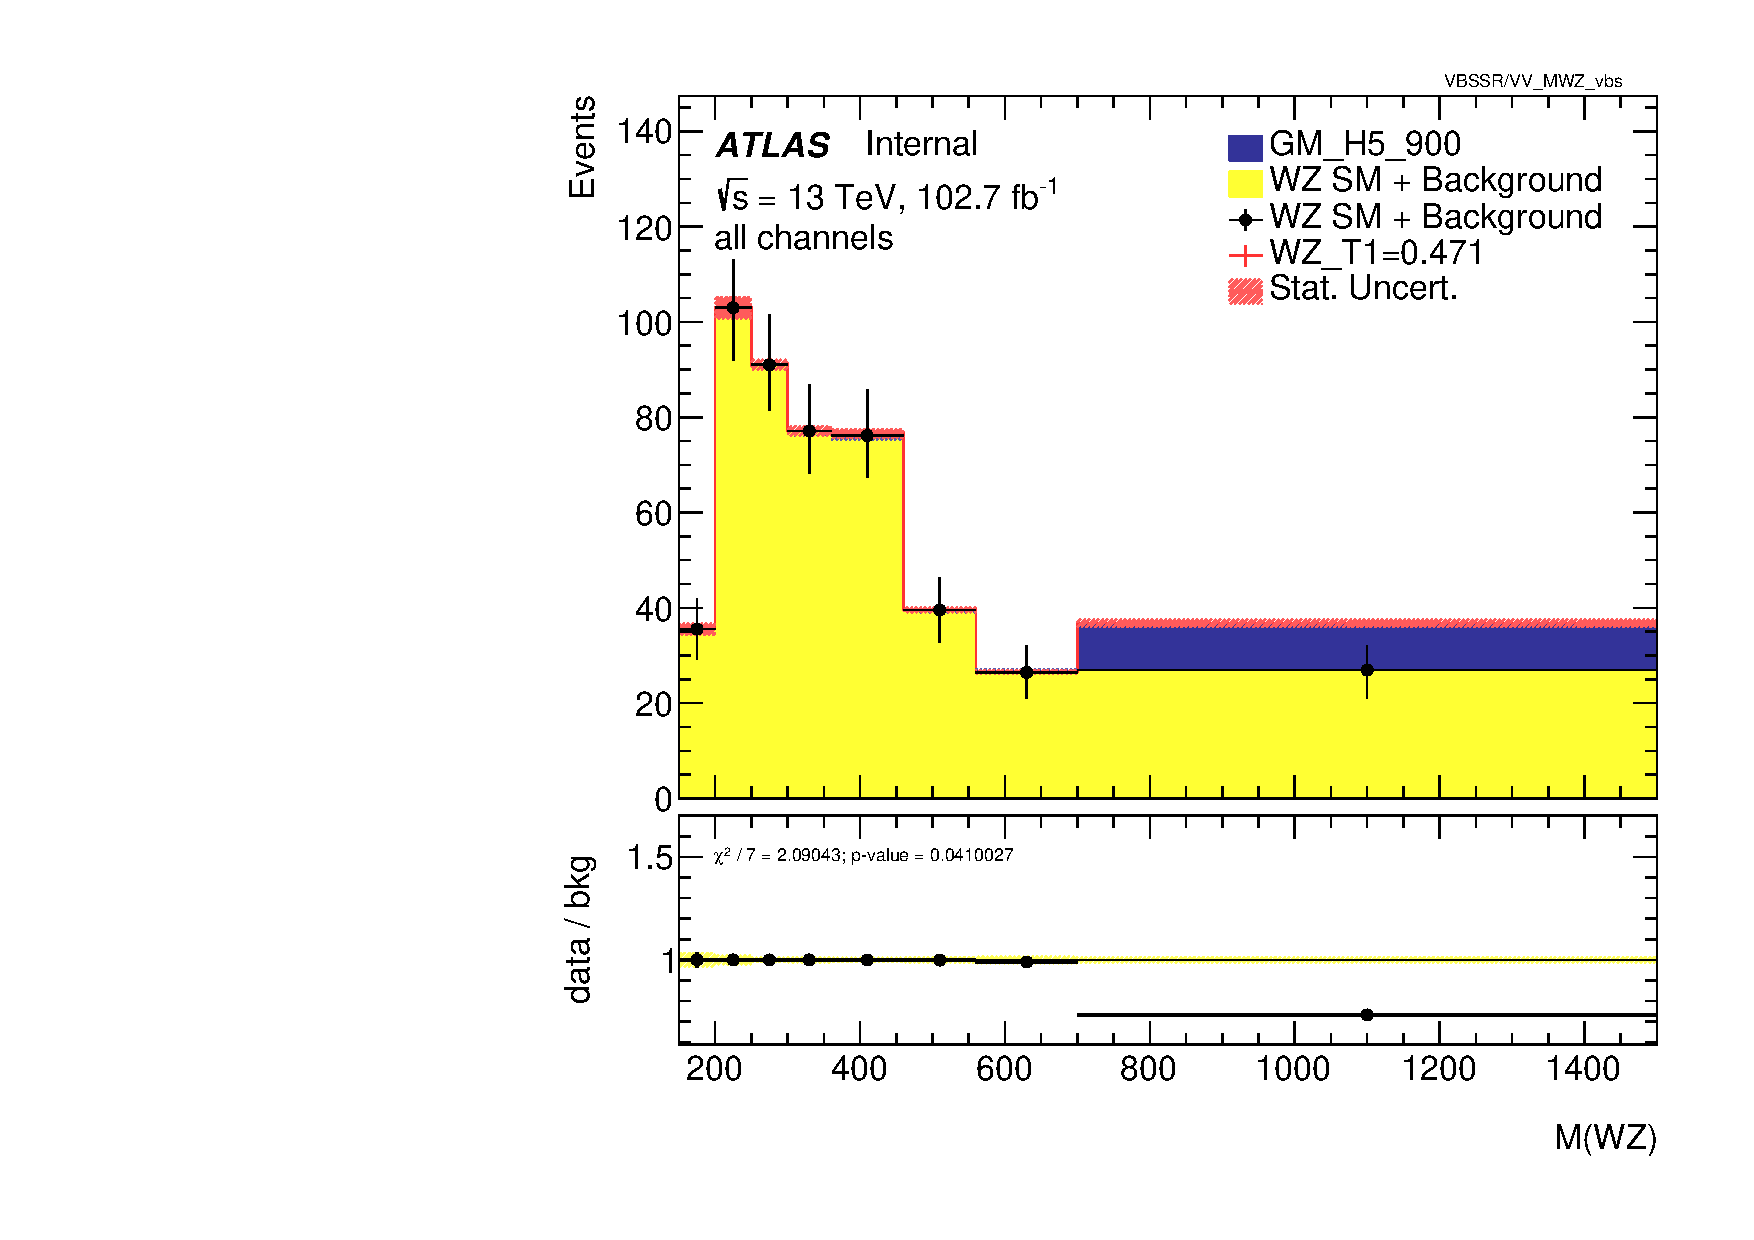
\includegraphics[width=\textwidth]{Plots/ALL_MWZ_right_color/GM_H5_900/T1/2022-05-07/VBSSR/all_VV_MWZ_vbs.pdf}
    \end{subfigure}
    \begin{subfigure}{0.45\textwidth}
        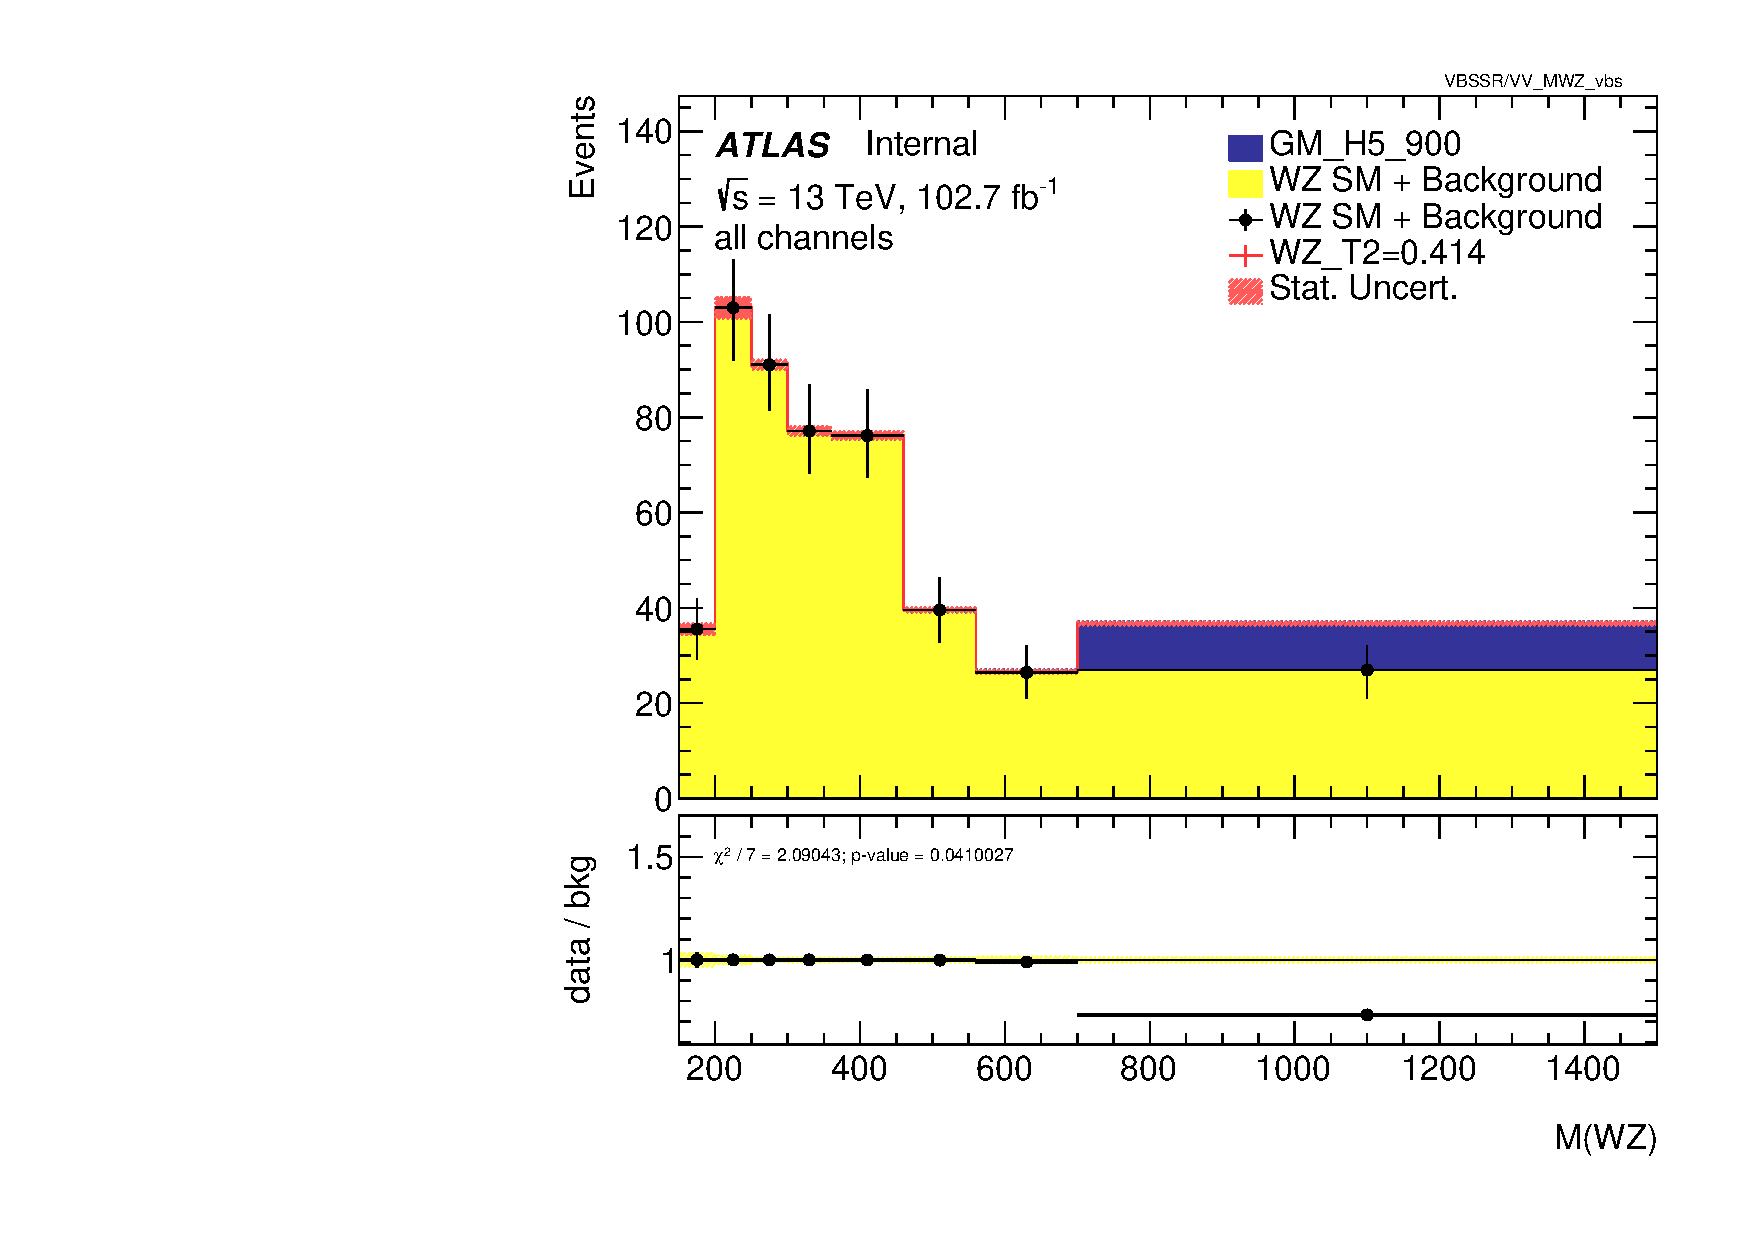
\includegraphics[width=\textwidth]{Plots/ALL_MWZ_right_color/GM_H5_900/T2/2022-05-07/VBSSR/all_VV_MWZ_vbs.pdf}
    \end{subfigure}

    \caption{Invariant mass for parameters S1, M0, M1, T0, T1, T2 with best fit value for 900 GeV resonance}
    \label{fig:all_mwz_900}
\end{figure}

\begin{figure}[h]

    \centering
    \begin{subfigure}{0.45\textwidth}
        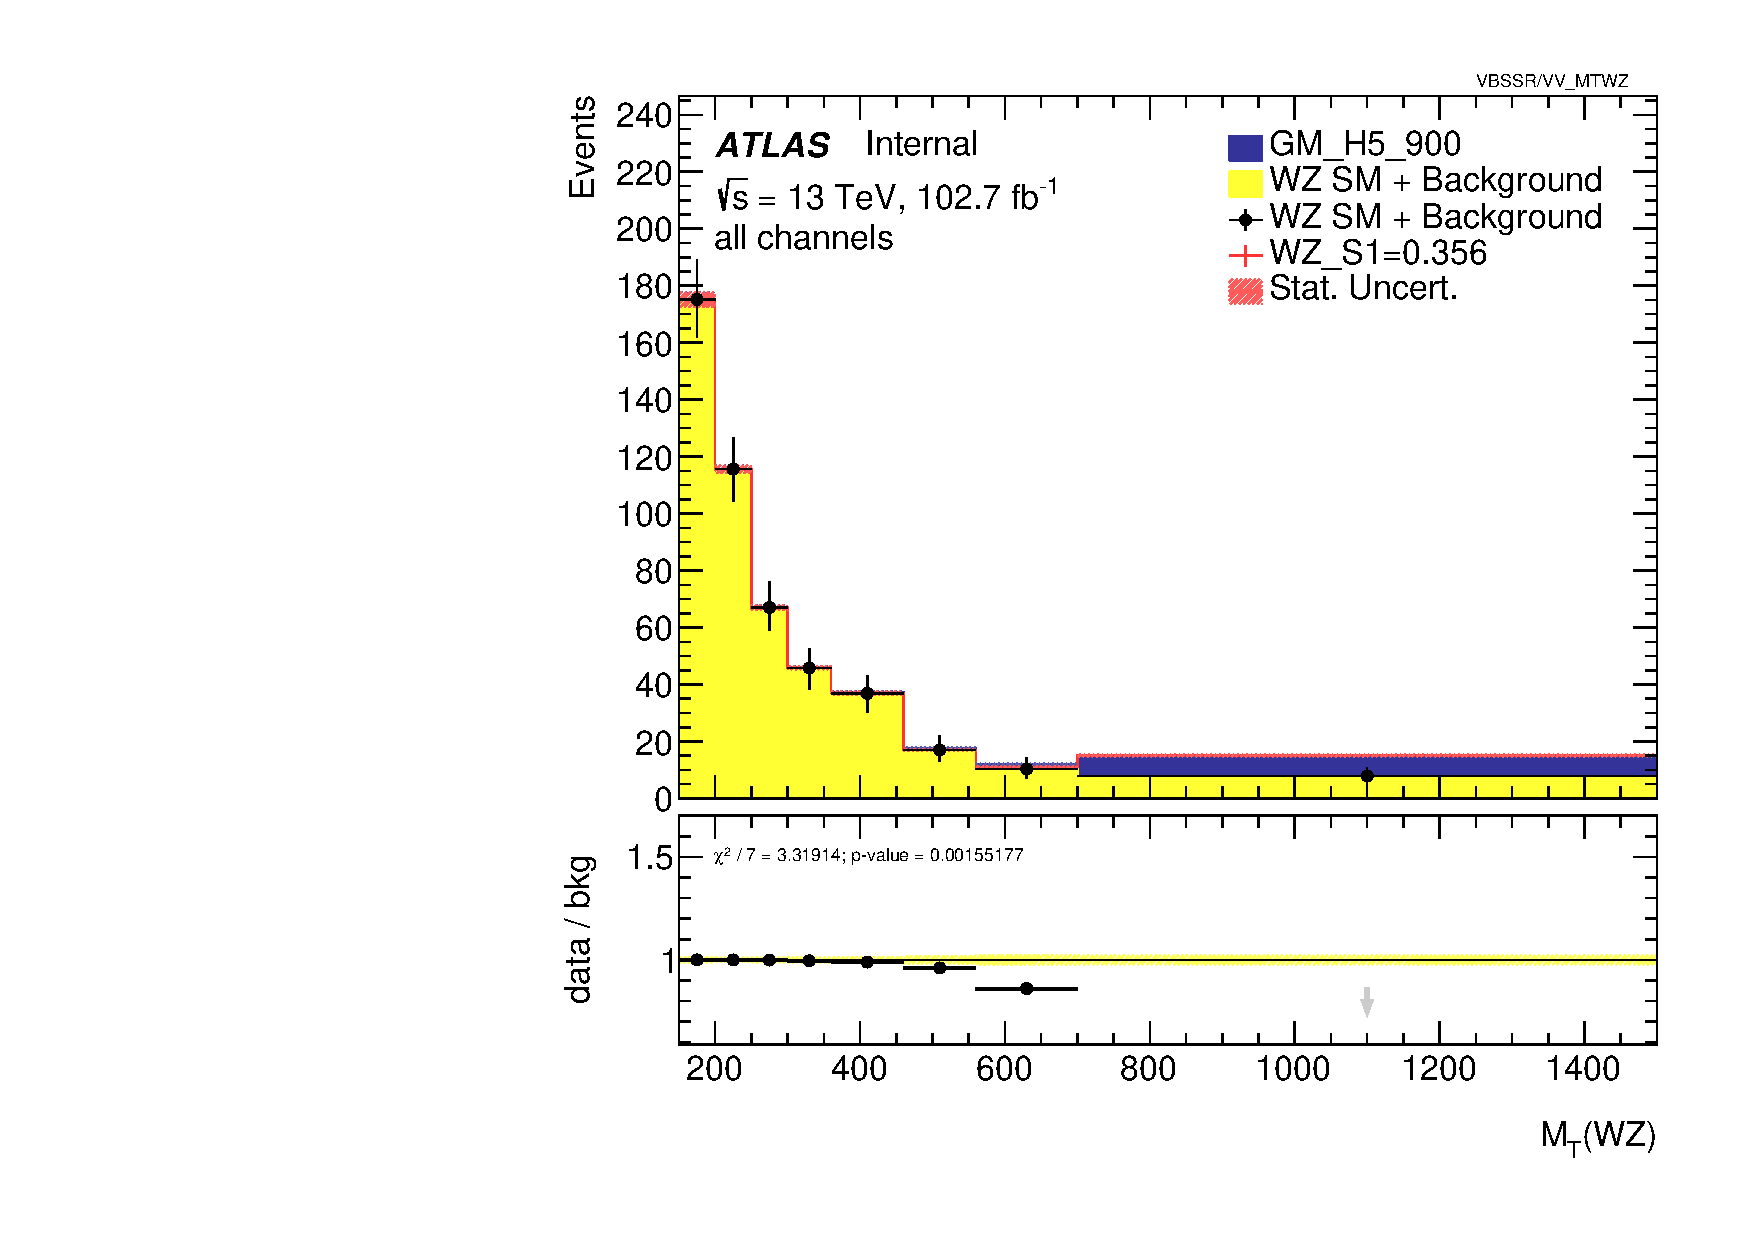
\includegraphics[width=\textwidth]{Plots/ALL_MTWZ_right_color/GM_H5_900/S1/2022-05-07/VBSSR/all_VV_MTWZ.pdf}
    \end{subfigure}
    \begin{subfigure}{0.45\textwidth}
        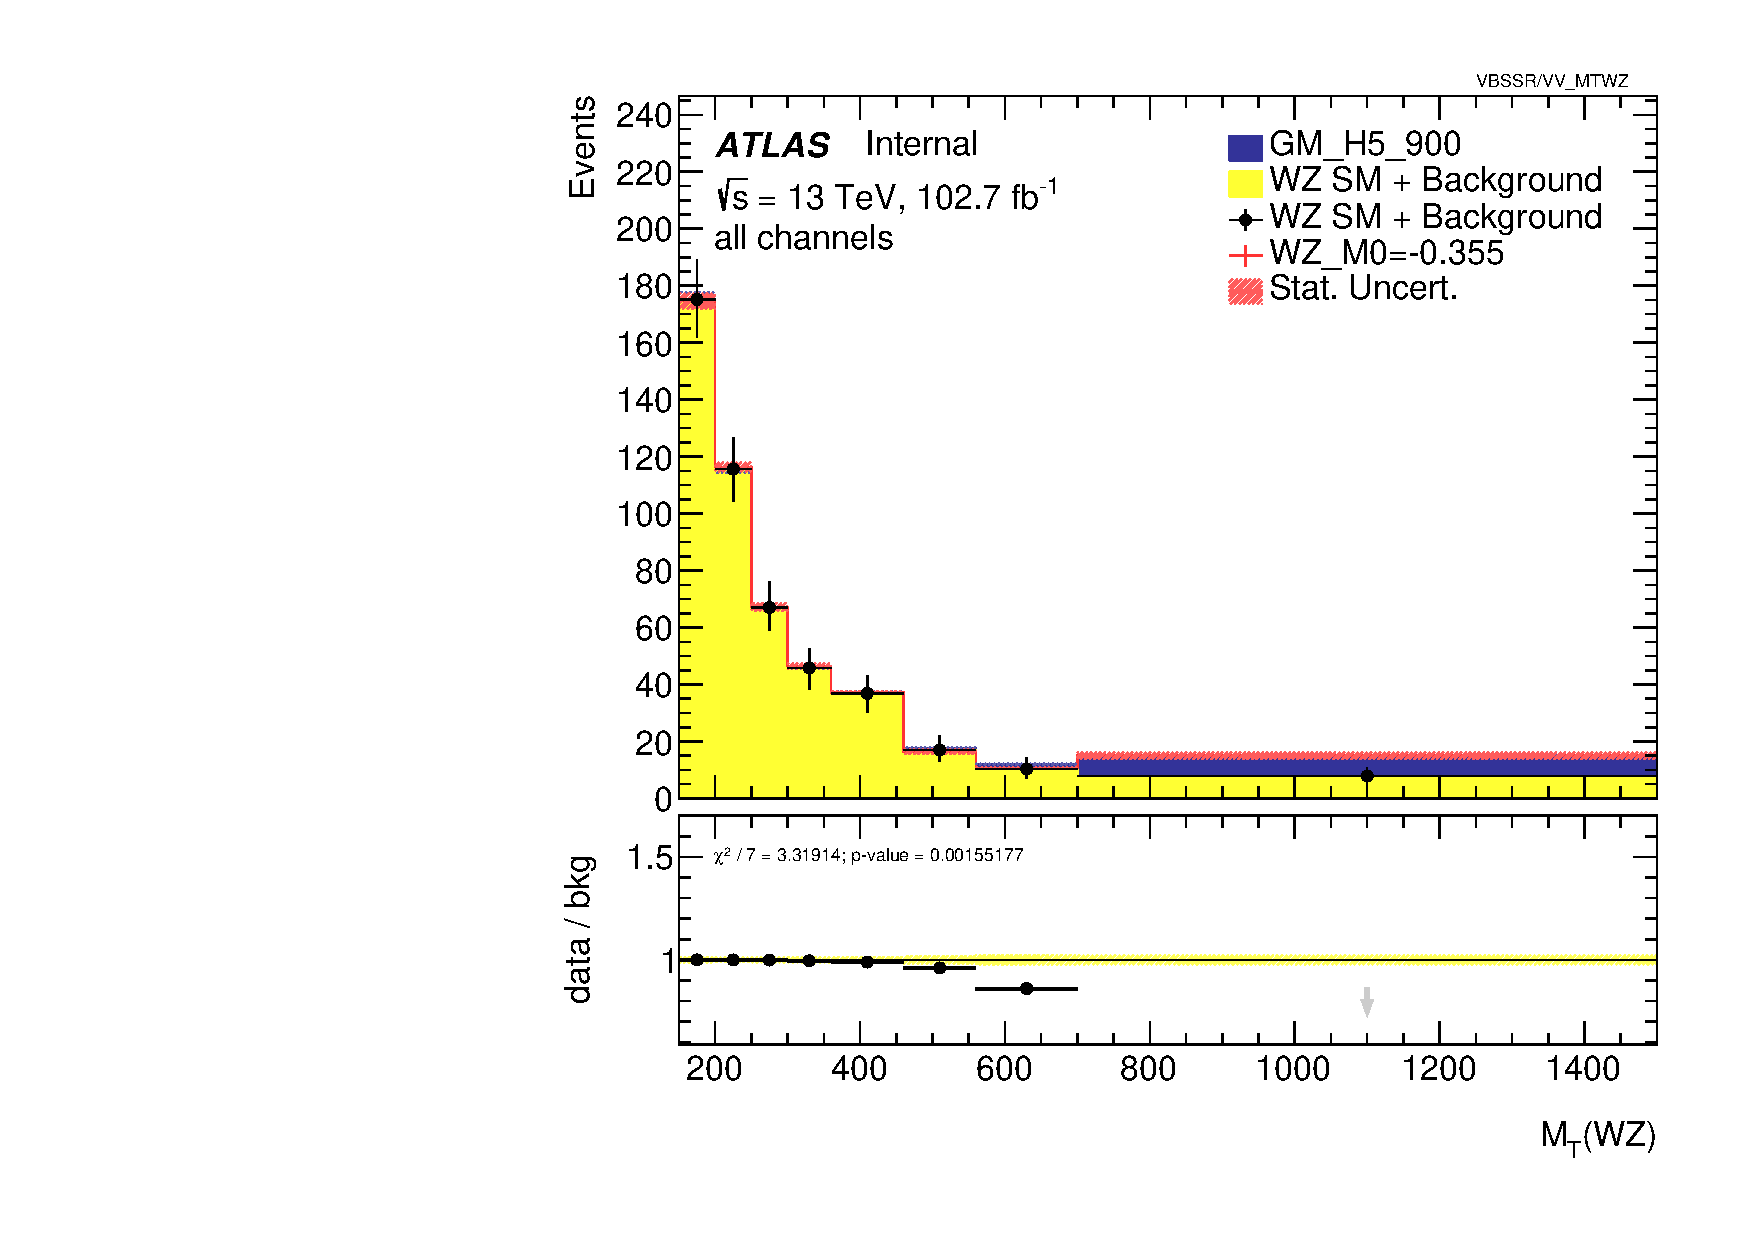
\includegraphics[width=\textwidth]{Plots/ALL_MTWZ_right_color/GM_H5_900/M0/2022-05-07/VBSSR/all_VV_MTWZ.pdf}
    \end{subfigure}
    \begin{subfigure}{0.45\textwidth}
        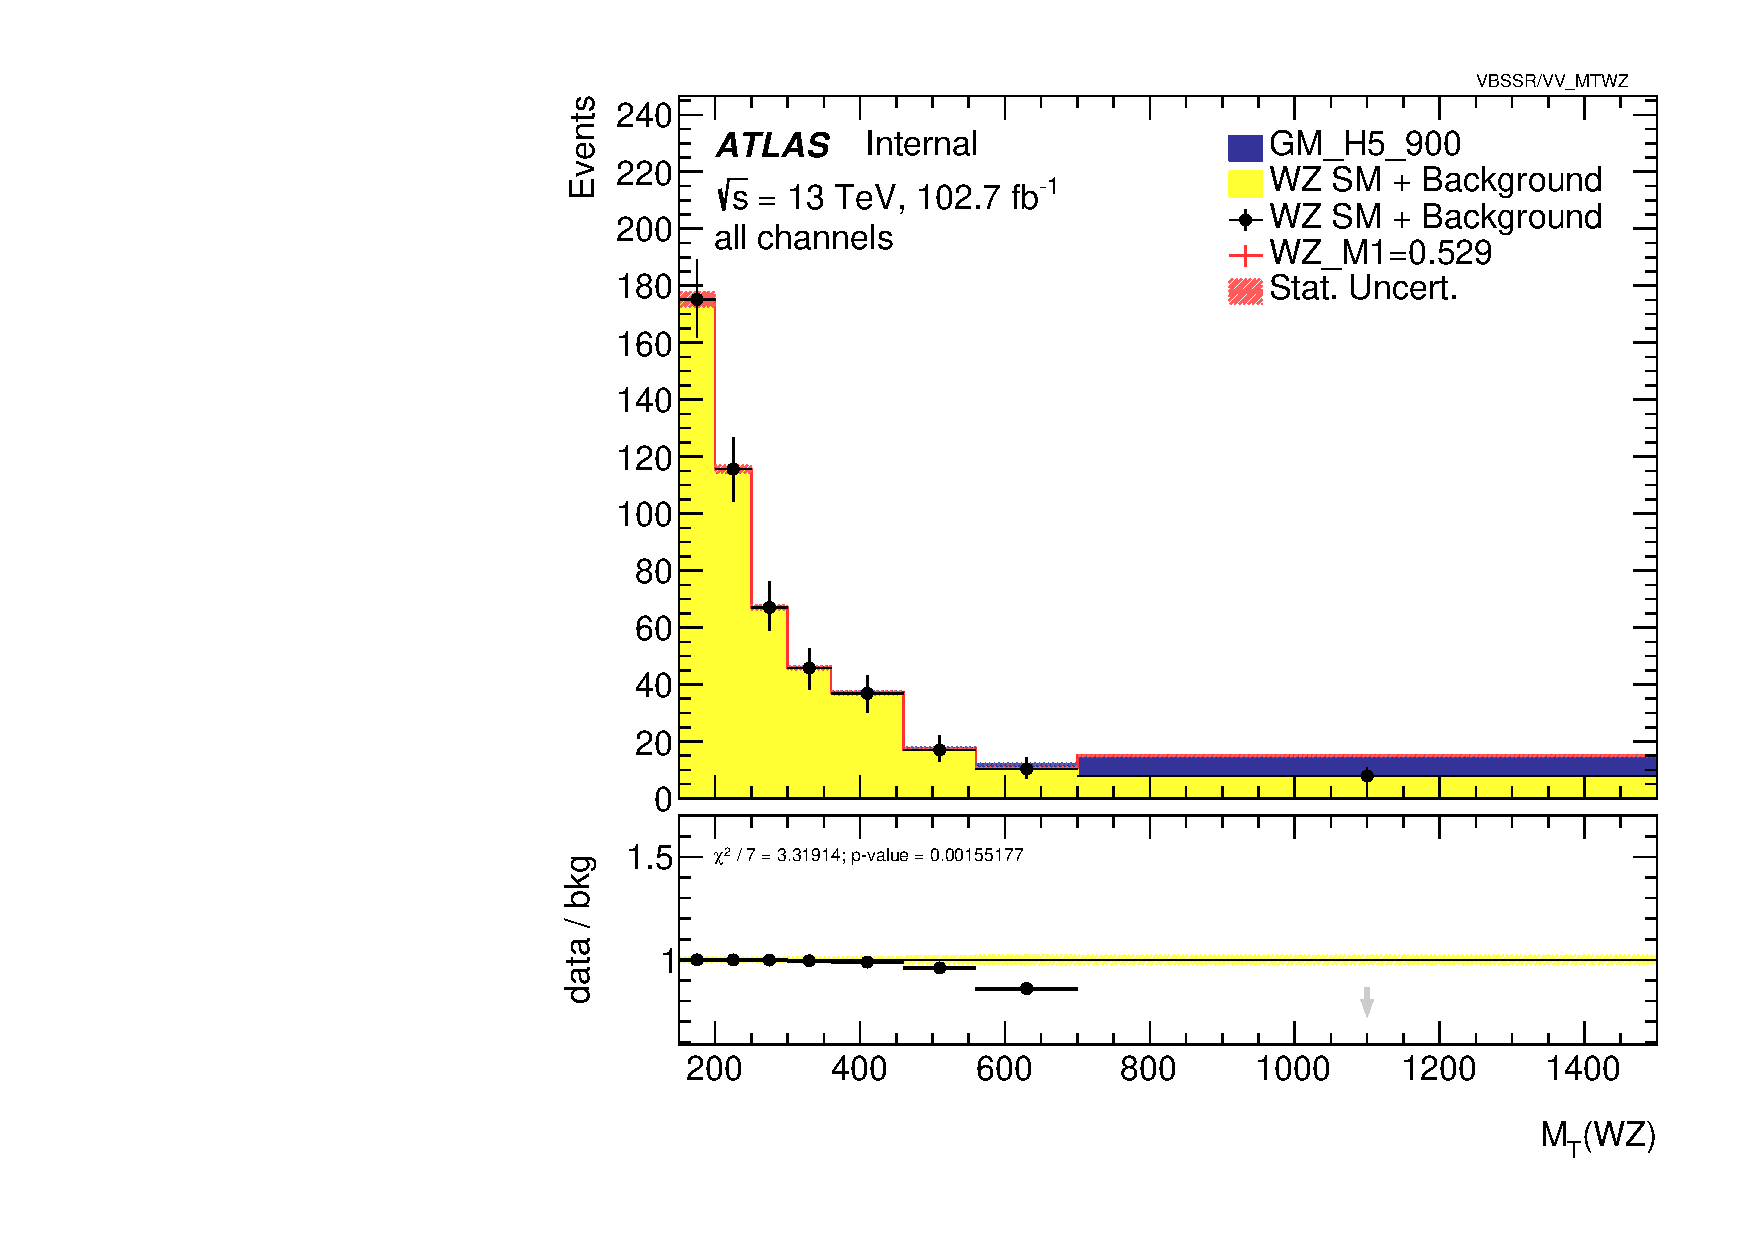
\includegraphics[width=\textwidth]{Plots/ALL_MTWZ_right_color/GM_H5_900/M1/2022-05-07/VBSSR/all_VV_MTWZ.pdf}
    \end{subfigure}
    \begin{subfigure}{0.45\textwidth}
        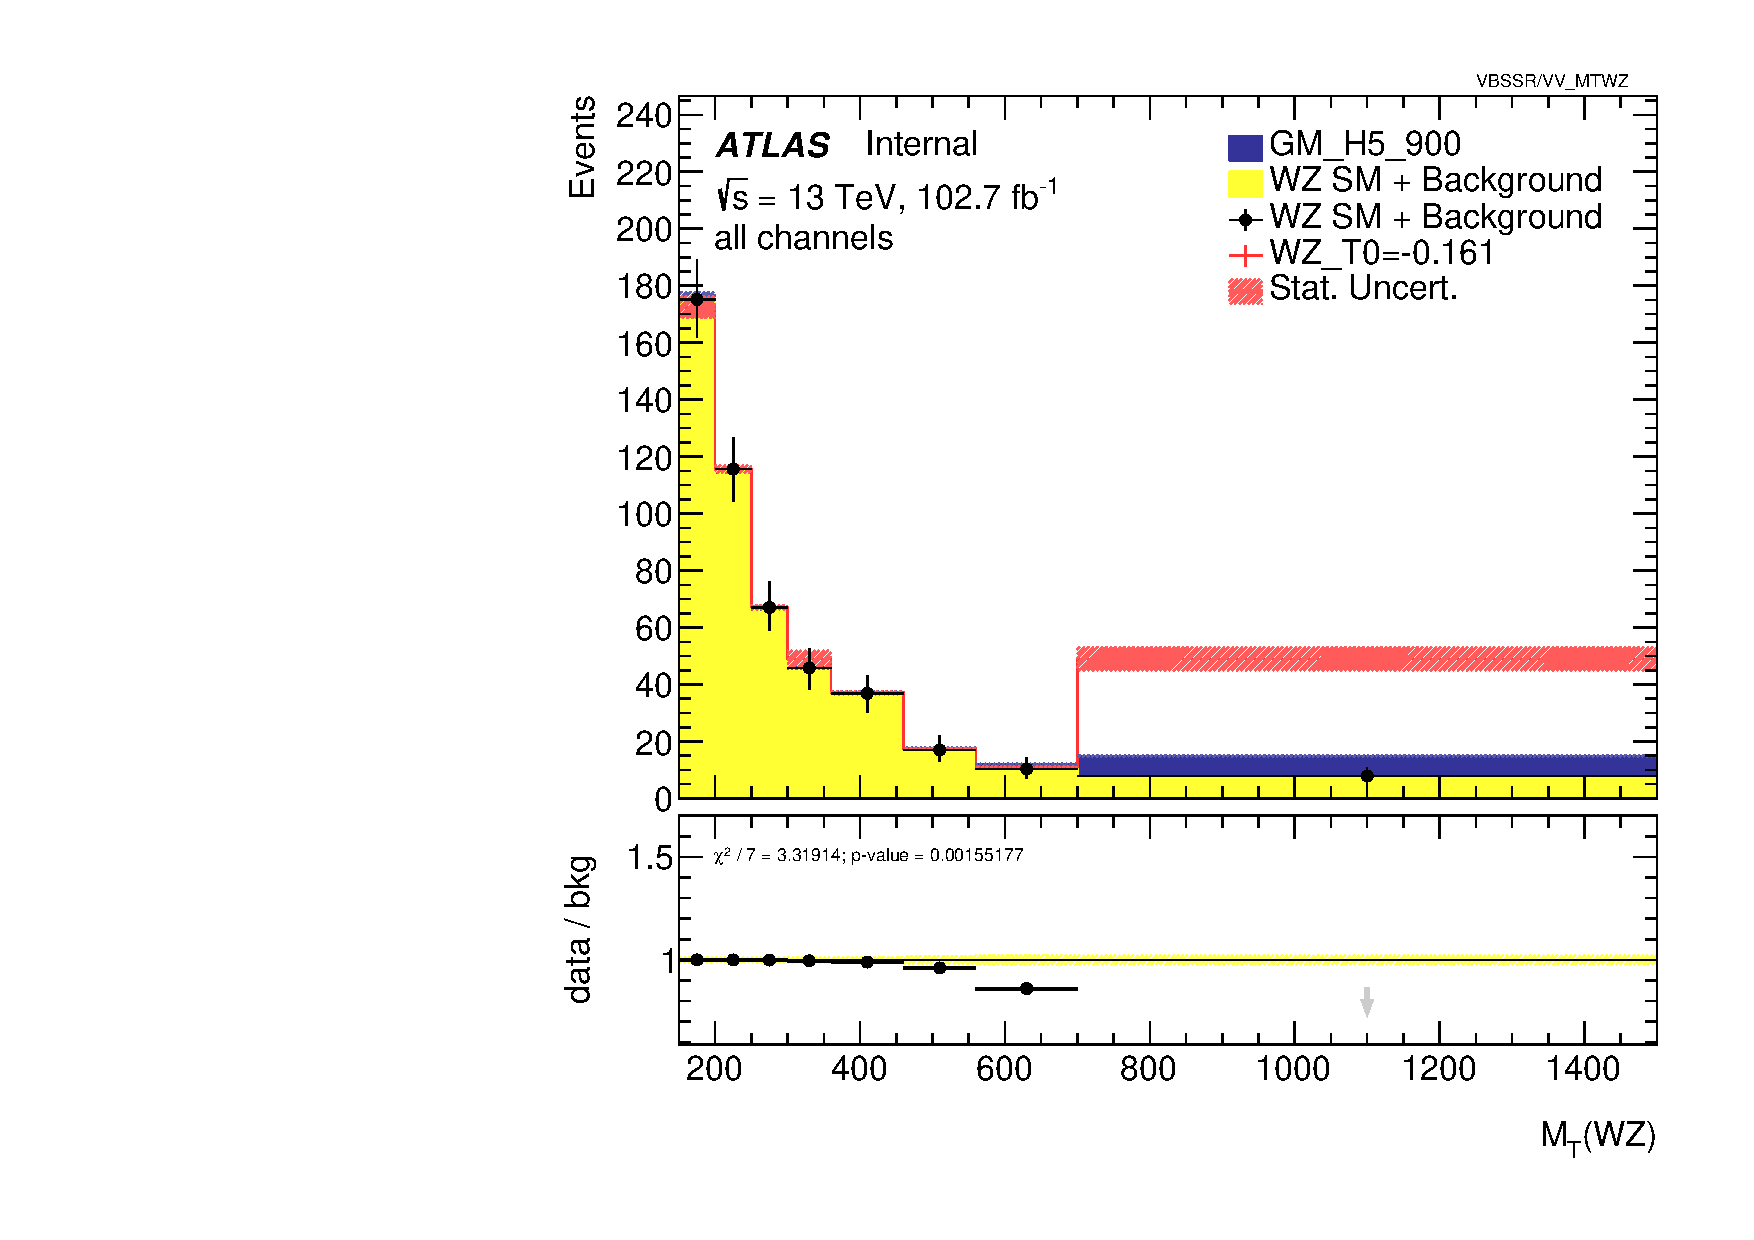
\includegraphics[width=\textwidth]{Plots/ALL_MTWZ_right_color/GM_H5_900/T0/2022-05-07/VBSSR/all_VV_MTWZ.pdf}
    \end{subfigure}
    \begin{subfigure}{0.45\textwidth}
        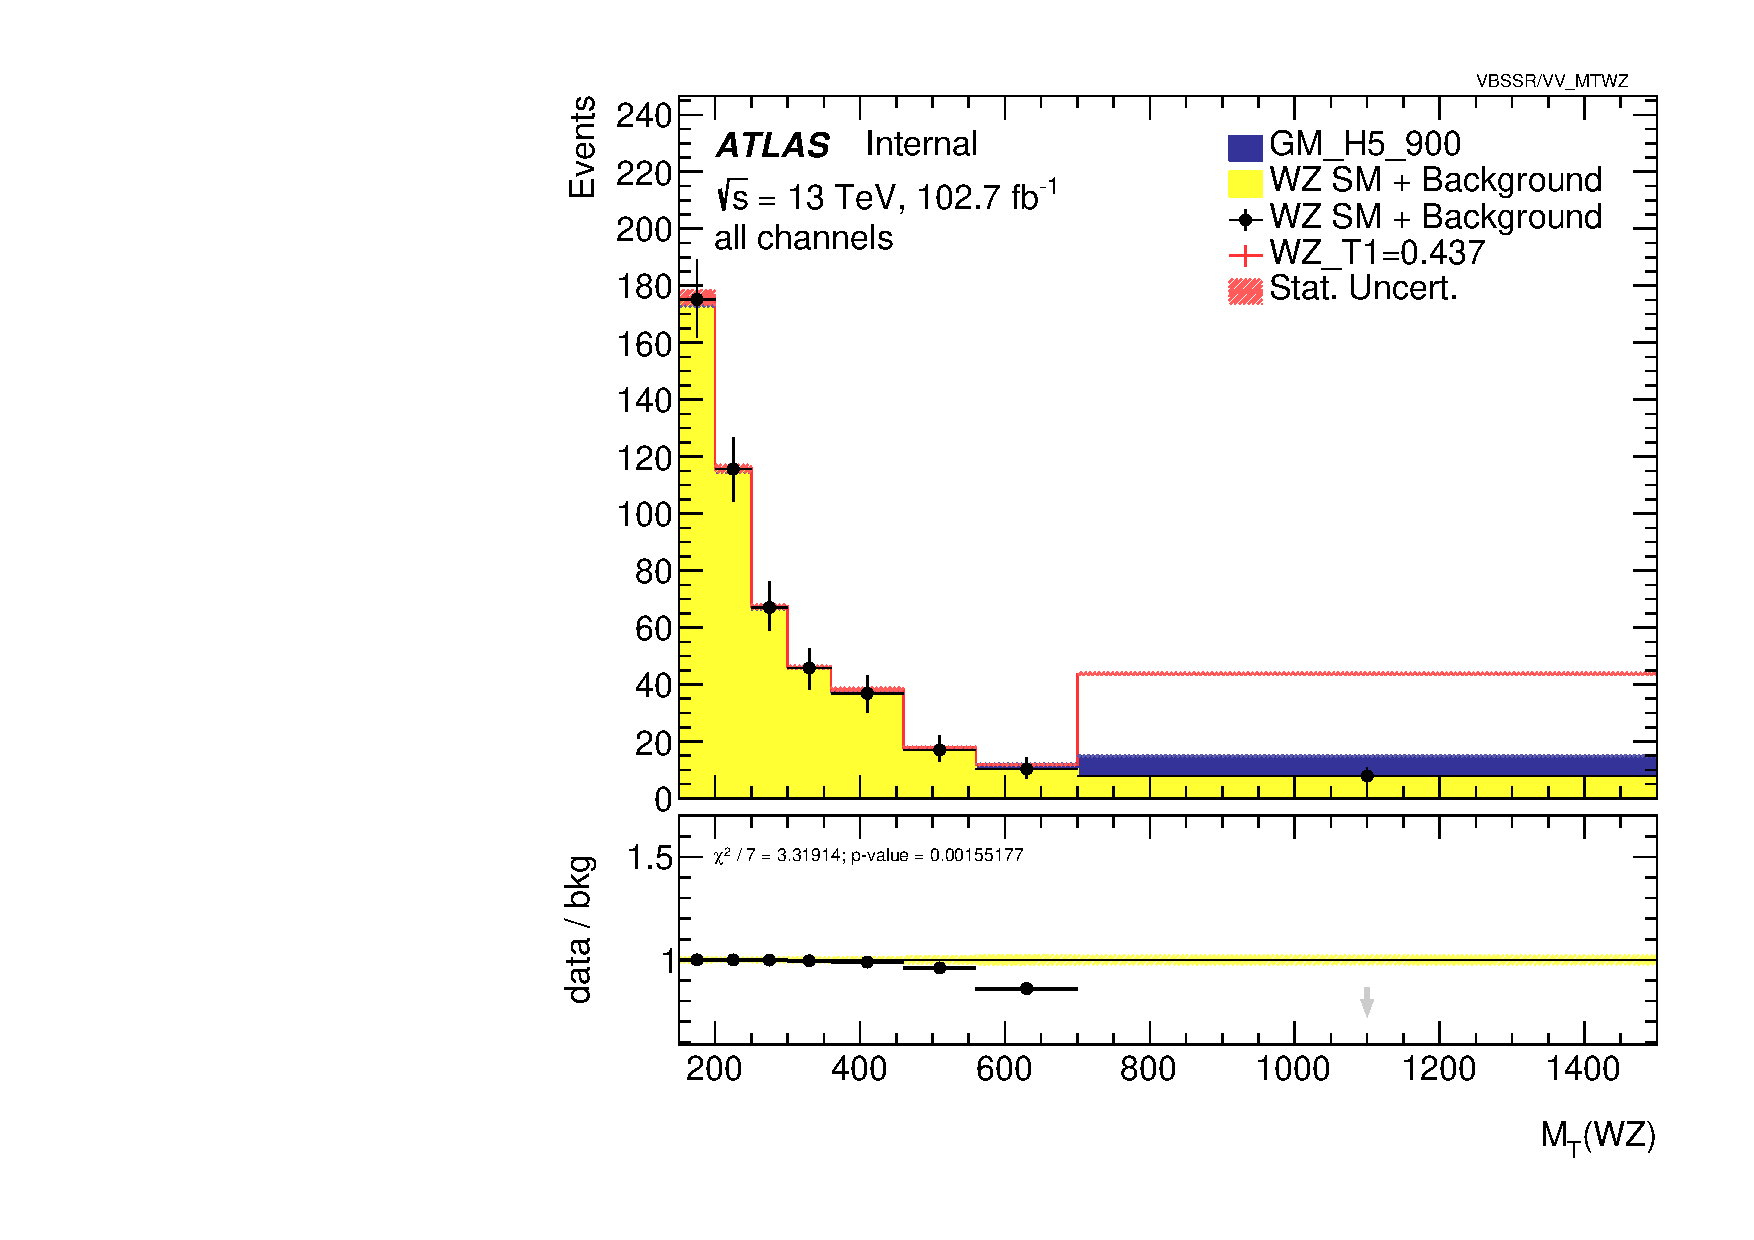
\includegraphics[width=\textwidth]{Plots/ALL_MTWZ_right_color/GM_H5_900/T1/2022-05-07/VBSSR/all_VV_MTWZ.pdf}
    \end{subfigure}
    \begin{subfigure}{0.45\textwidth}
        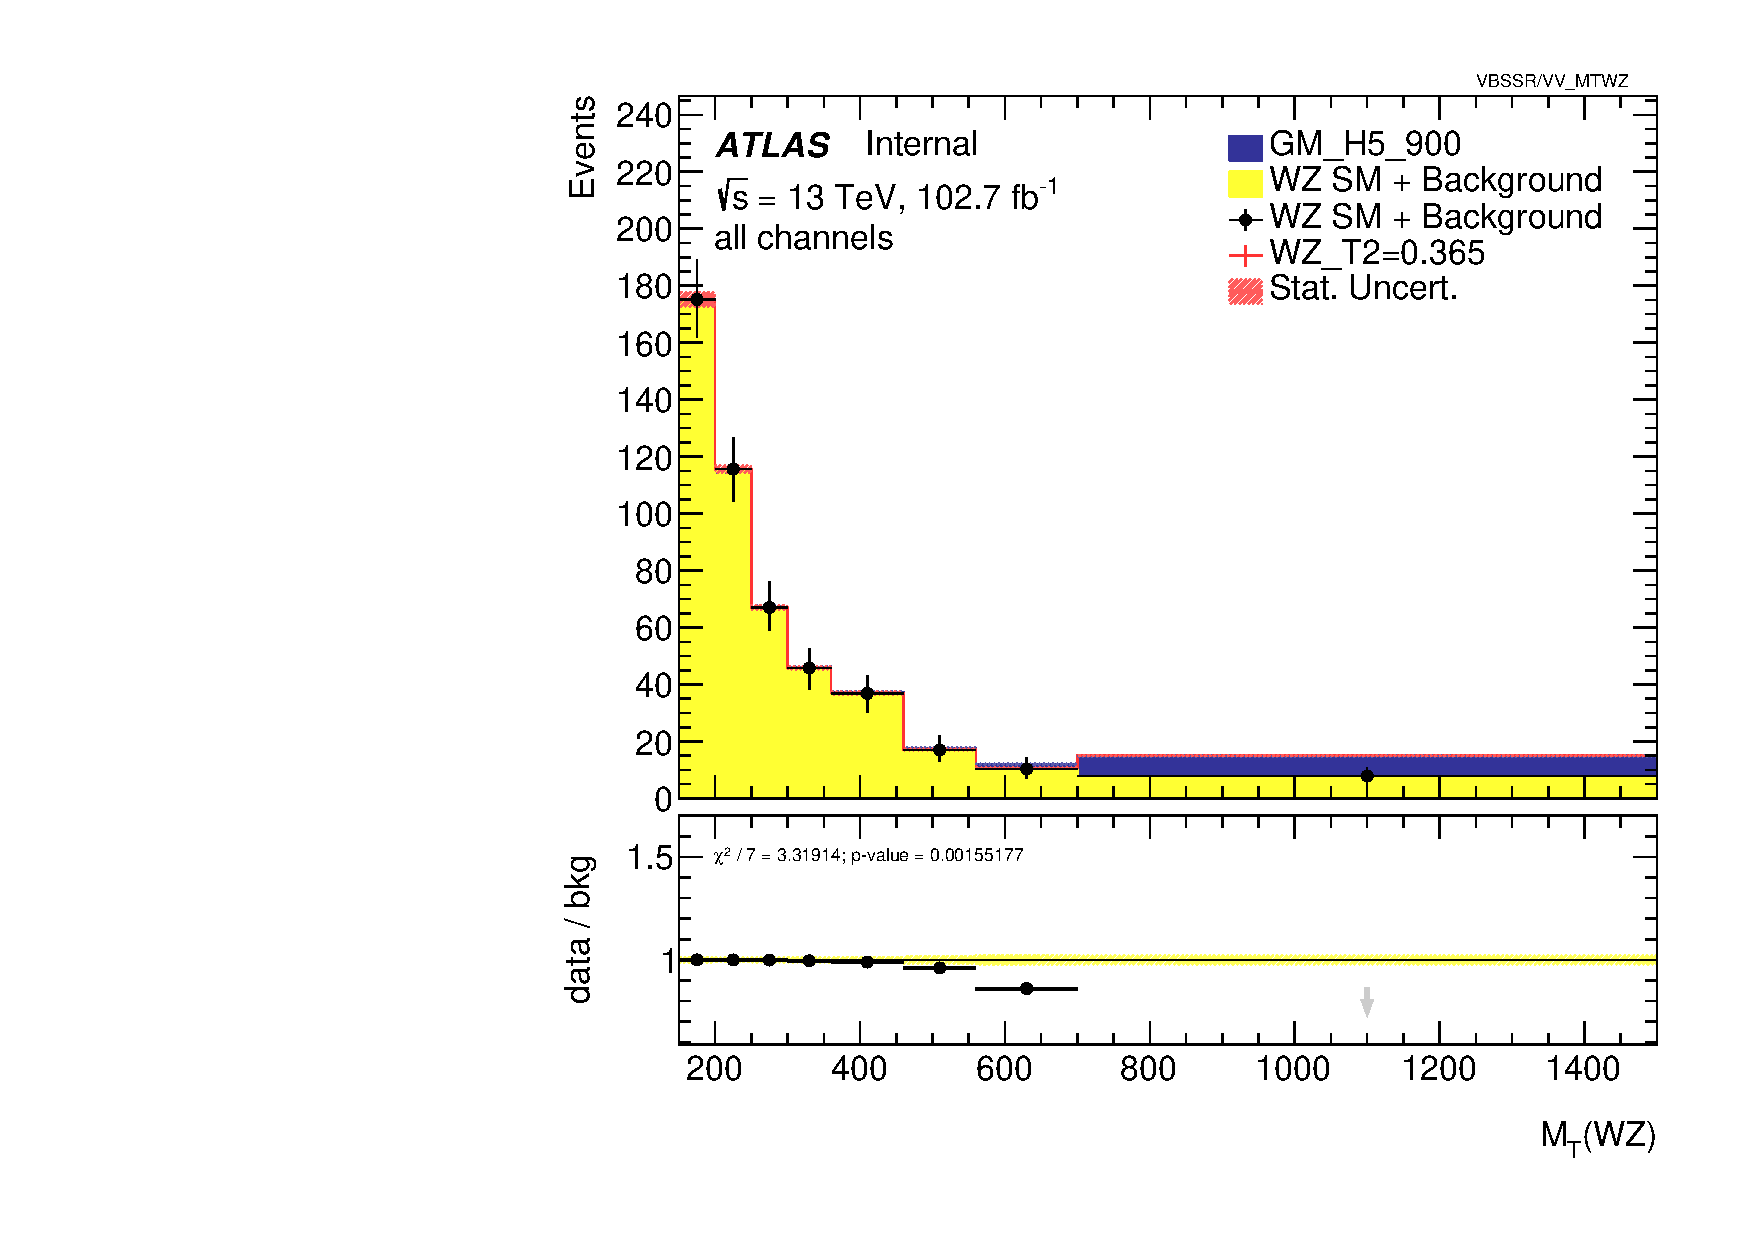
\includegraphics[width=\textwidth]{Plots/ALL_MTWZ_right_color/GM_H5_900/T2/2022-05-07/VBSSR/all_VV_MTWZ.pdf}
    \end{subfigure}

    \caption{transverse mass for parameters S1, M0, M1, T0, T1, T2 with best fit value for 900 GeV resonance}
    \label{fig:all_mtwz_900}
\end{figure}
%--------------------------------------------------------------------------------------------------
\pagebreak
\newpage

\subsection{1000 GeV resonance}

\begin{figure}[h]

    \centering
    \begin{subfigure}{0.45\textwidth}
        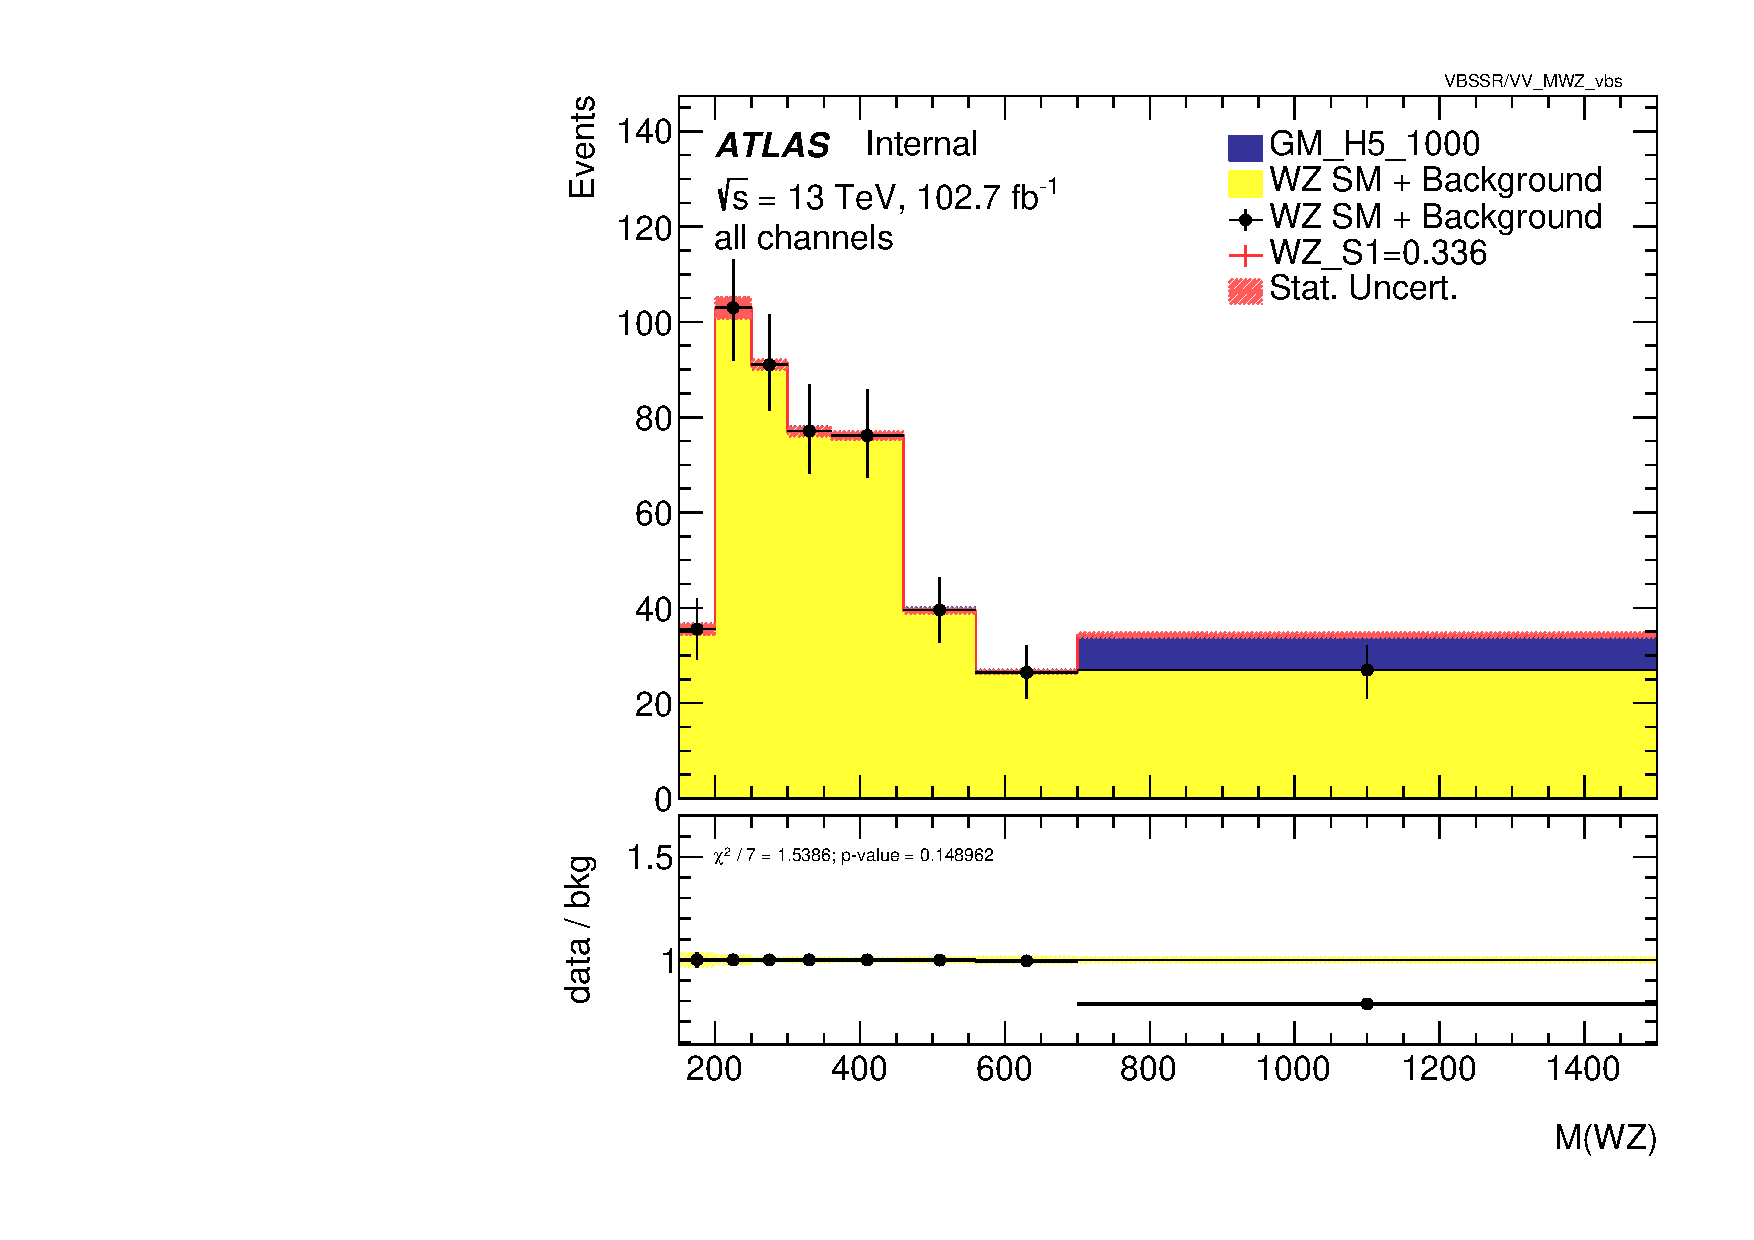
\includegraphics[width=\textwidth]{Plots/ALL_MWZ_right_color/GM_H5_1000/S1/2022-05-07/VBSSR/all_VV_MWZ_vbs.pdf}
    \end{subfigure}
    \begin{subfigure}{0.45\textwidth}
        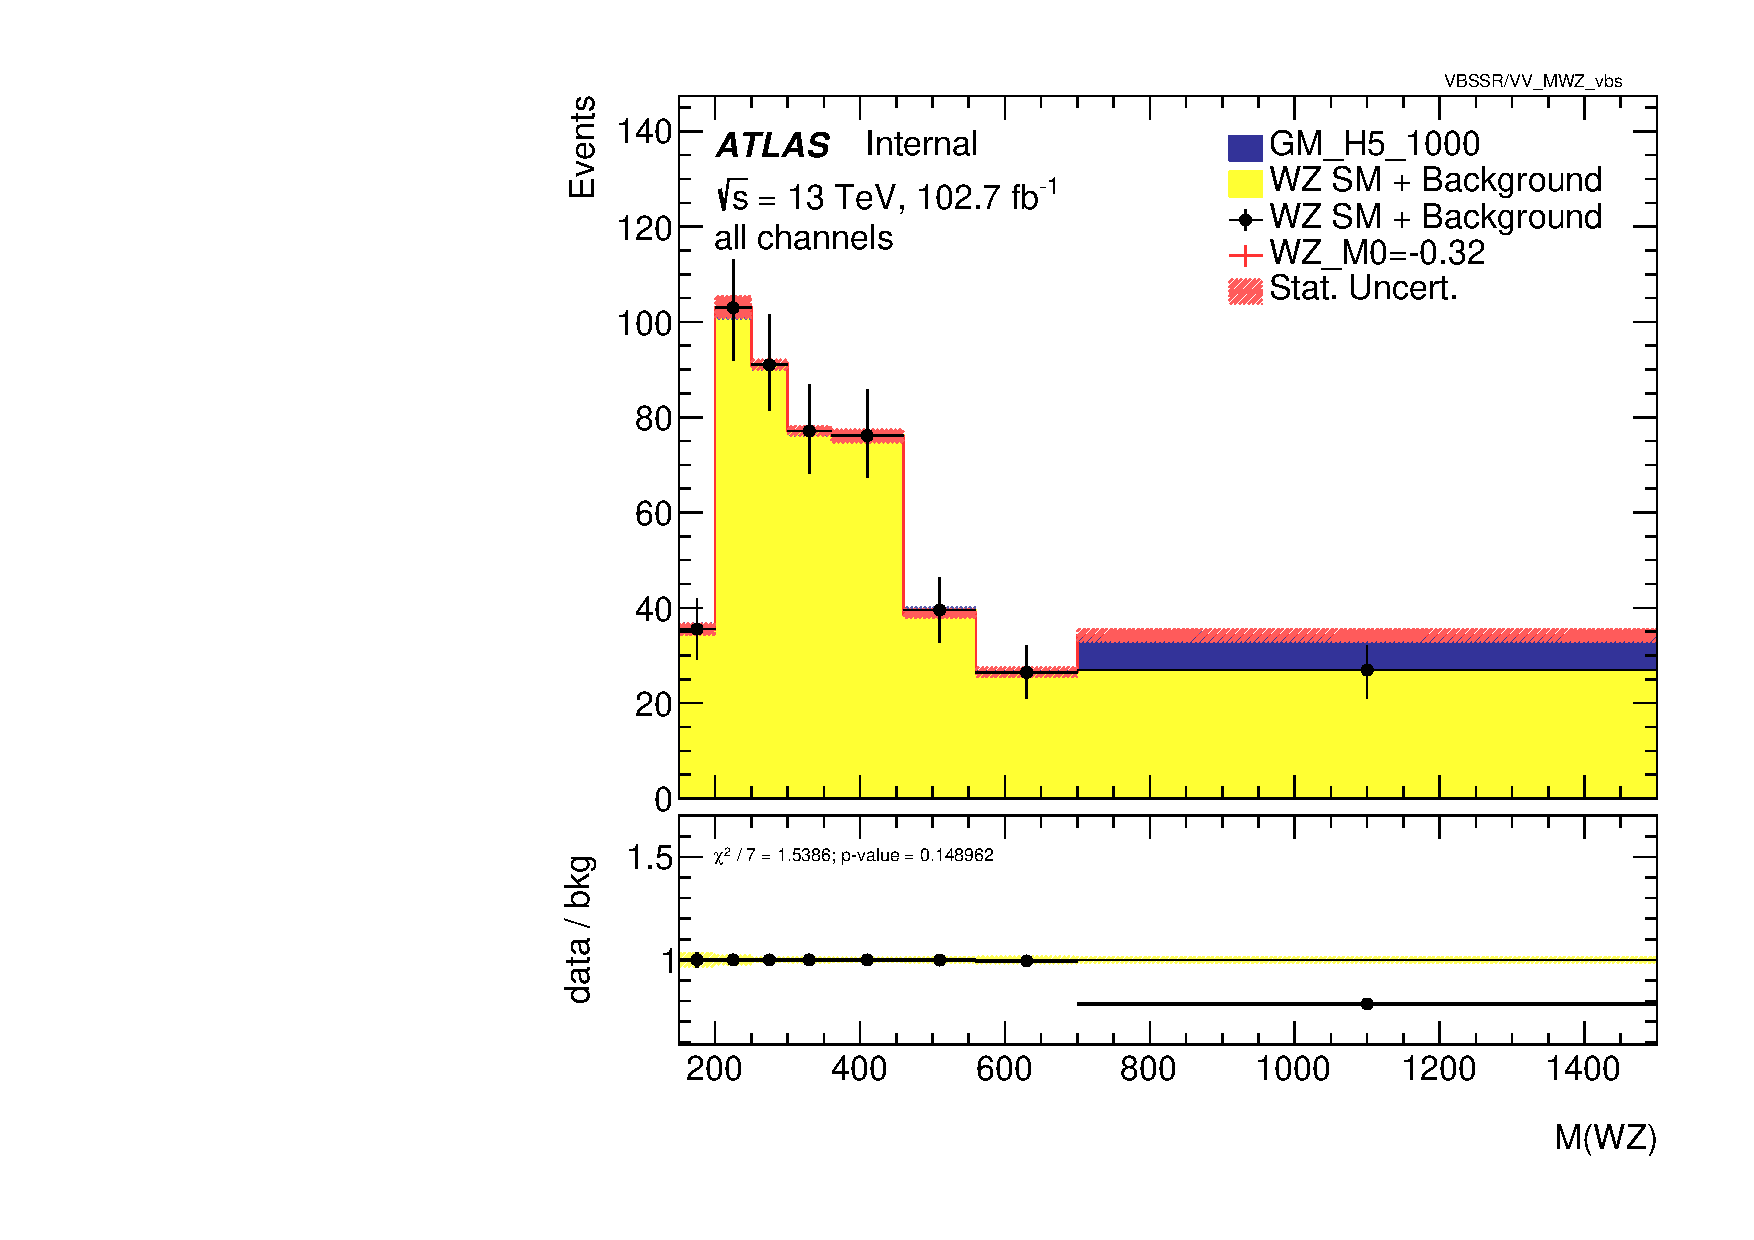
\includegraphics[width=\textwidth]{Plots/ALL_MWZ_right_color/GM_H5_1000/M0/2022-05-07/VBSSR/all_VV_MWZ_vbs.pdf}
    \end{subfigure}
    \begin{subfigure}{0.45\textwidth}
        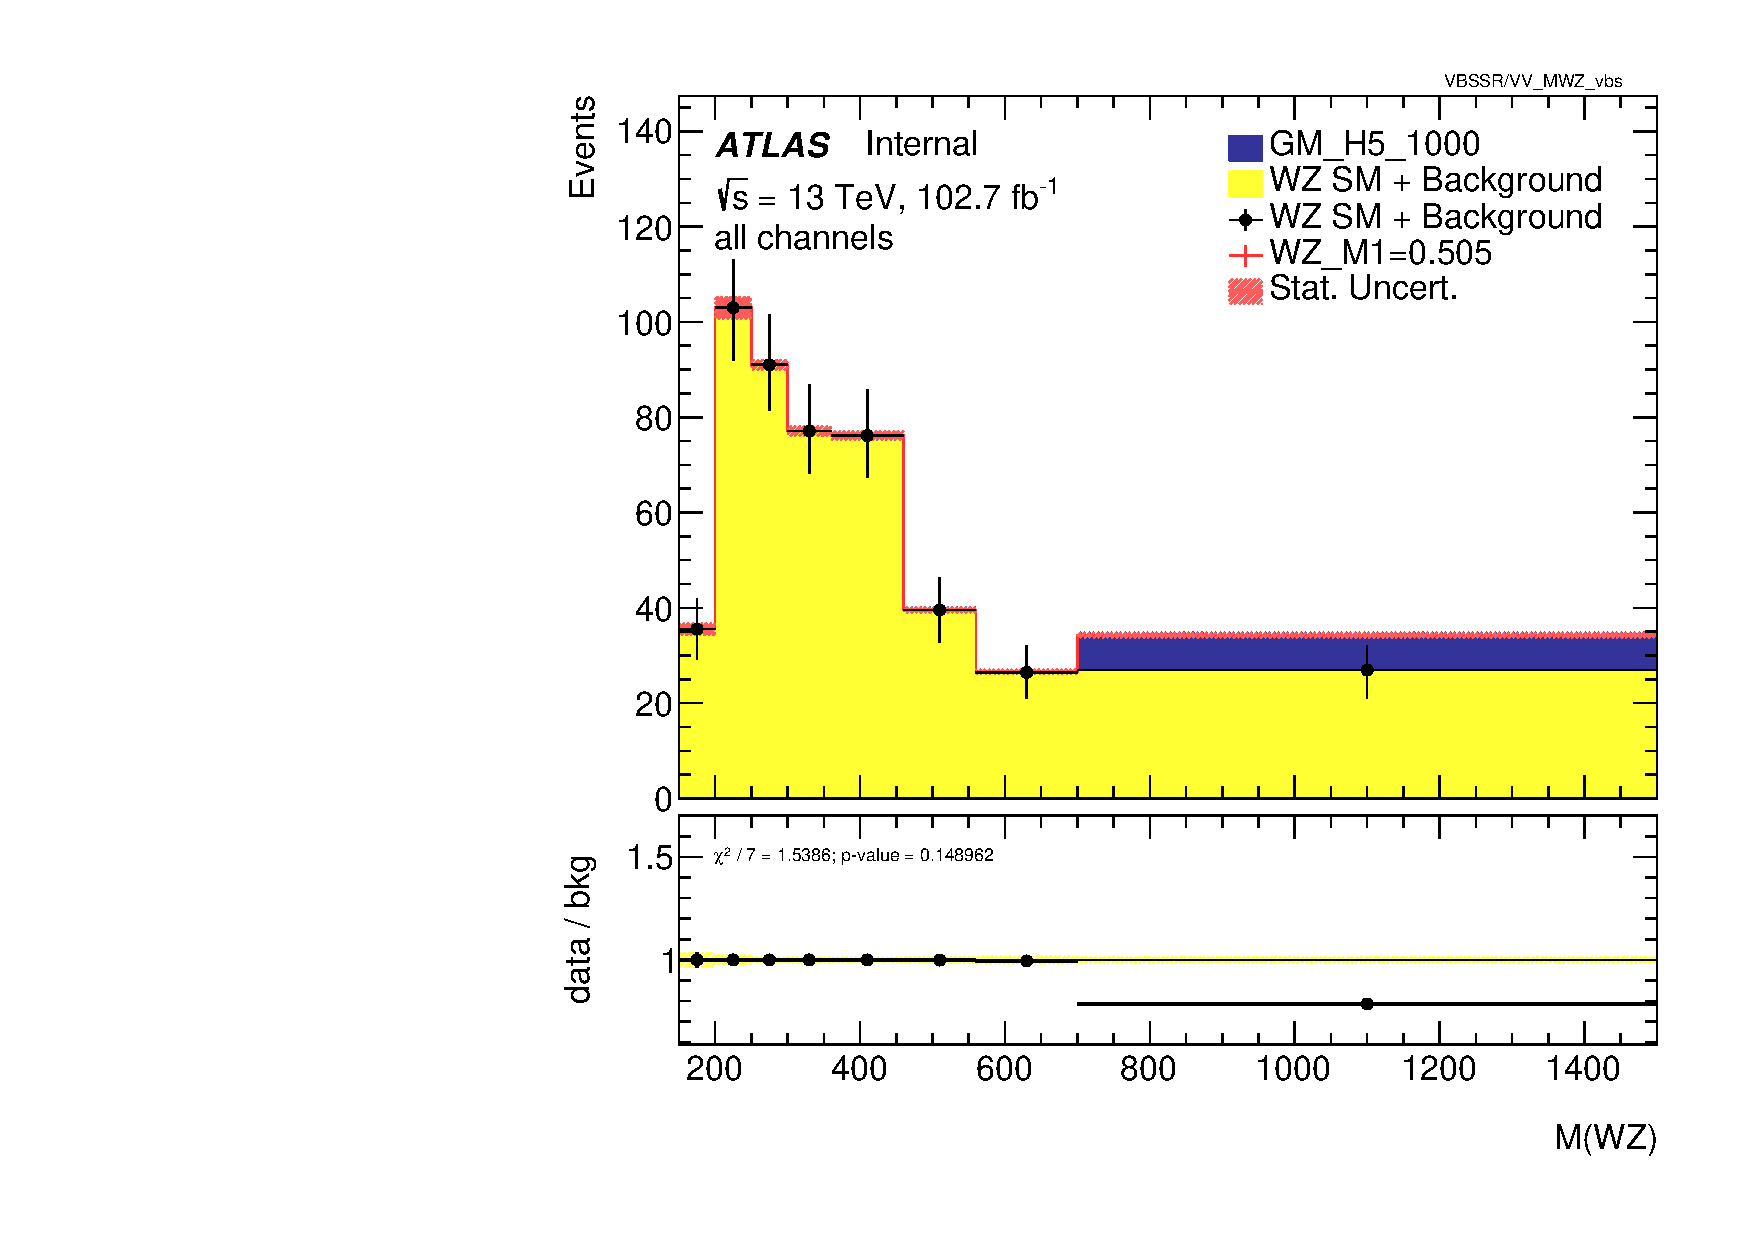
\includegraphics[width=\textwidth]{Plots/ALL_MWZ_right_color/GM_H5_1000/M1/2022-05-07/VBSSR/all_VV_MWZ_vbs.pdf}
    \end{subfigure}
    \begin{subfigure}{0.45\textwidth}
        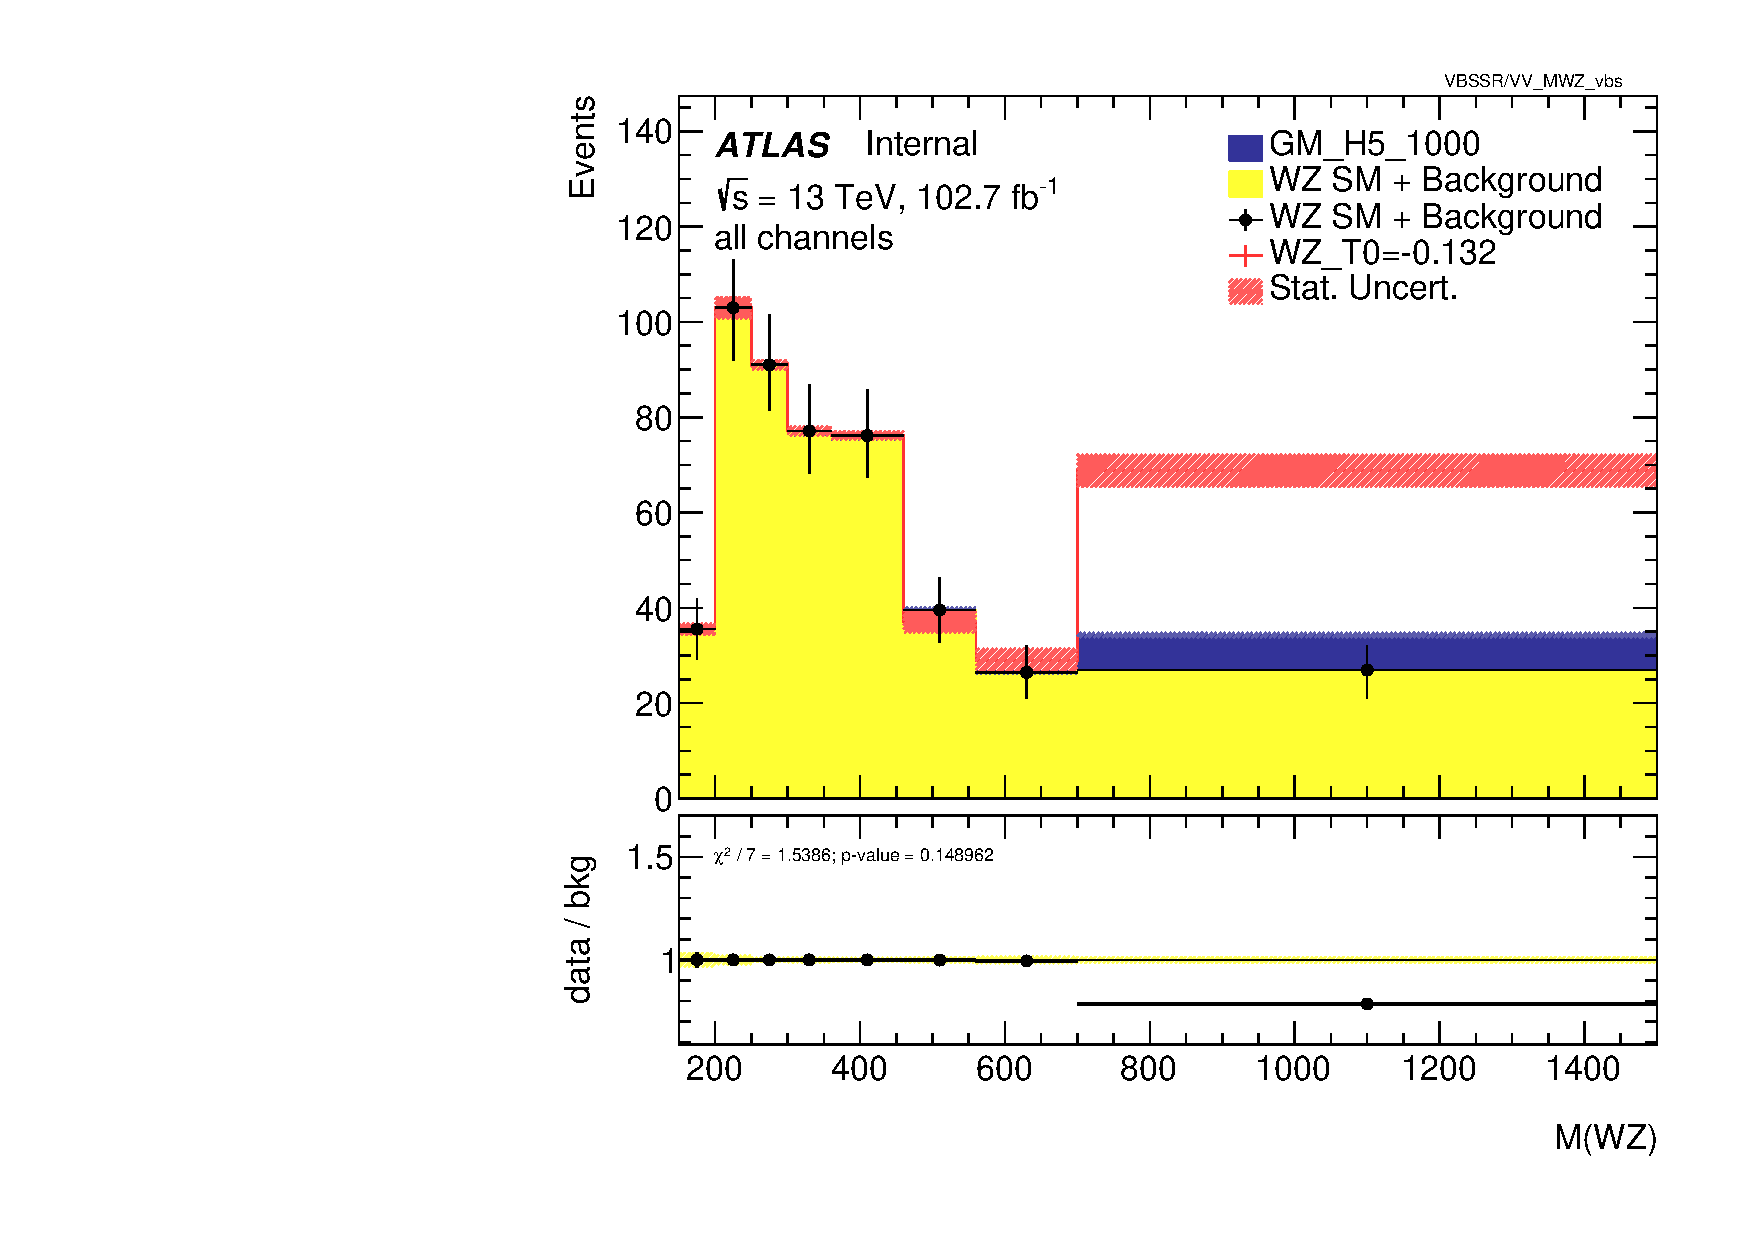
\includegraphics[width=\textwidth]{Plots/ALL_MWZ_right_color/GM_H5_1000/T0/2022-05-07/VBSSR/all_VV_MWZ_vbs.pdf}
    \end{subfigure}
    \begin{subfigure}{0.45\textwidth}
        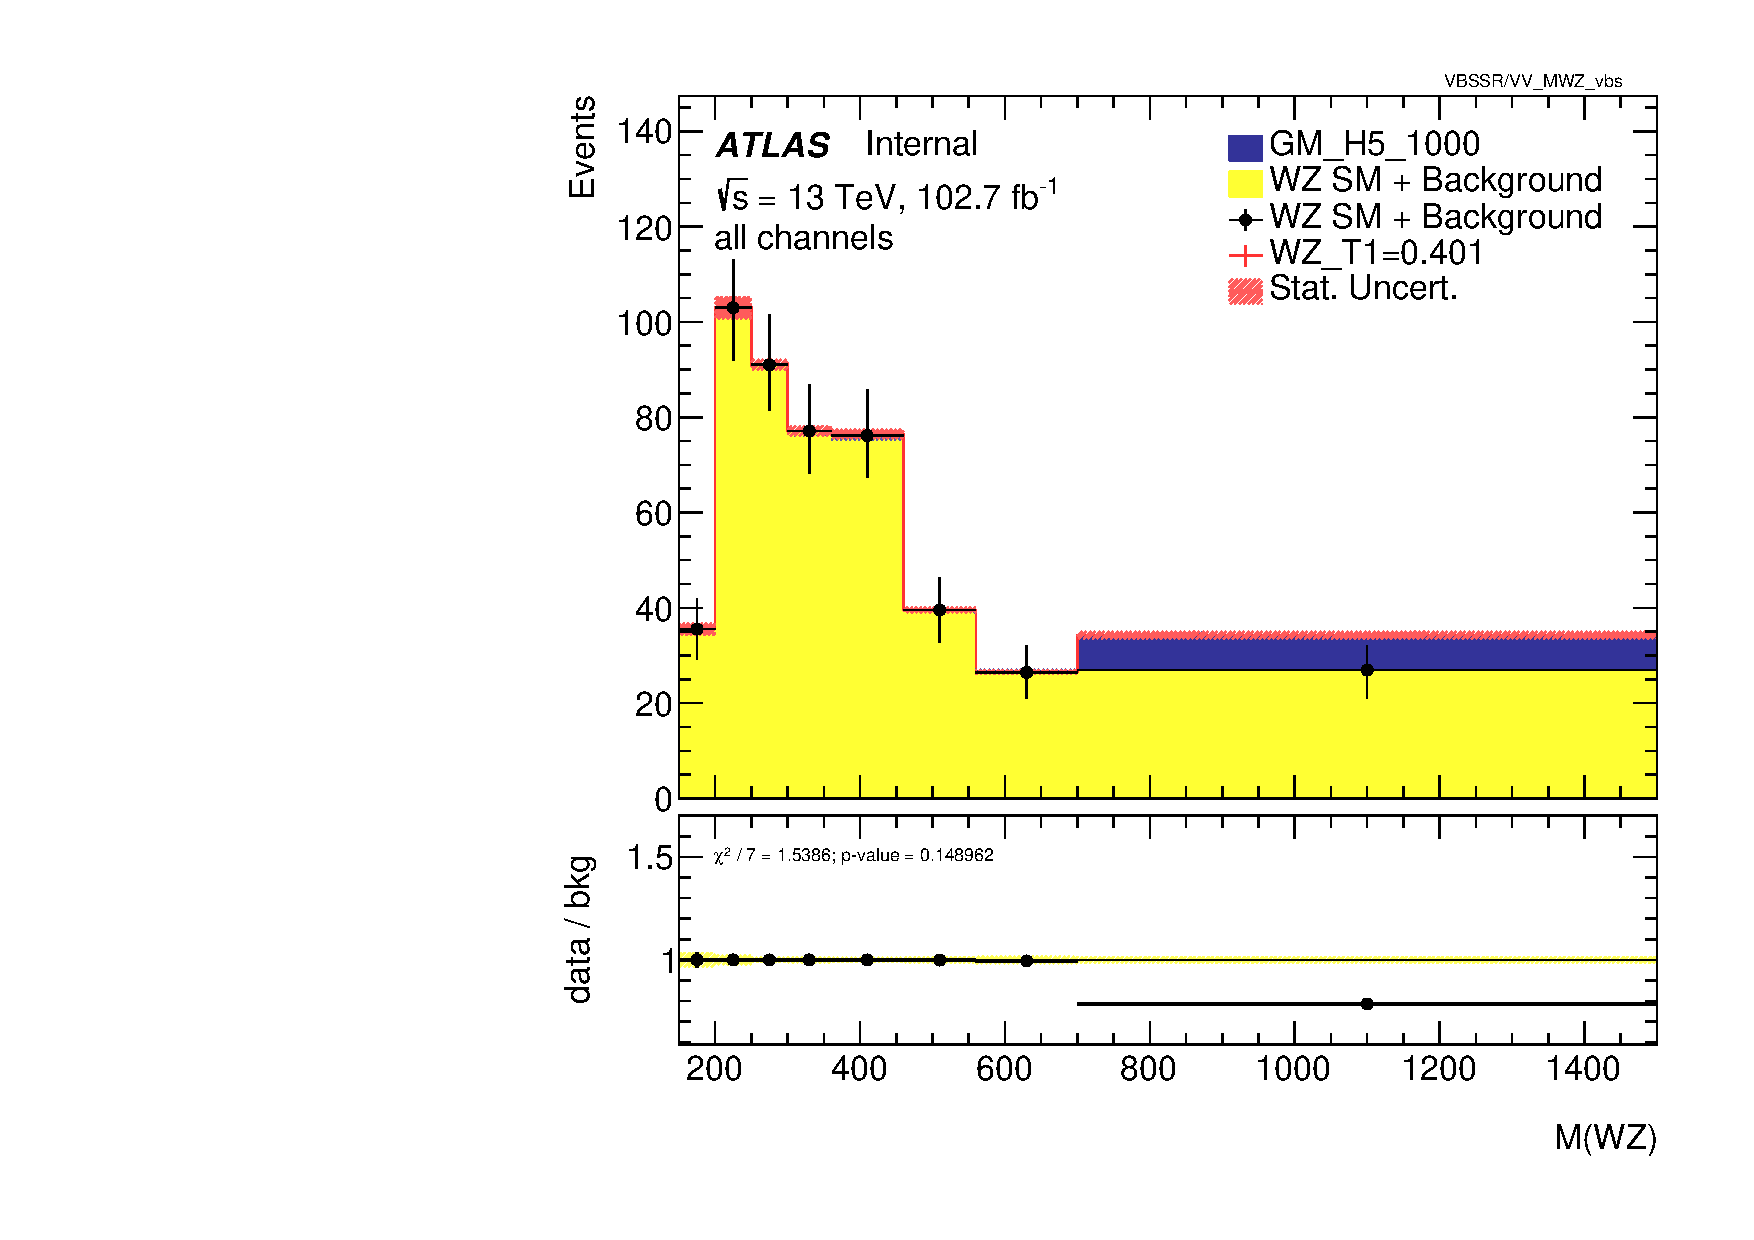
\includegraphics[width=\textwidth]{Plots/1000_T1_MWZ/all_VV_MWZ_vbs.pdf}
    \end{subfigure}
    \begin{subfigure}{0.45\textwidth}
        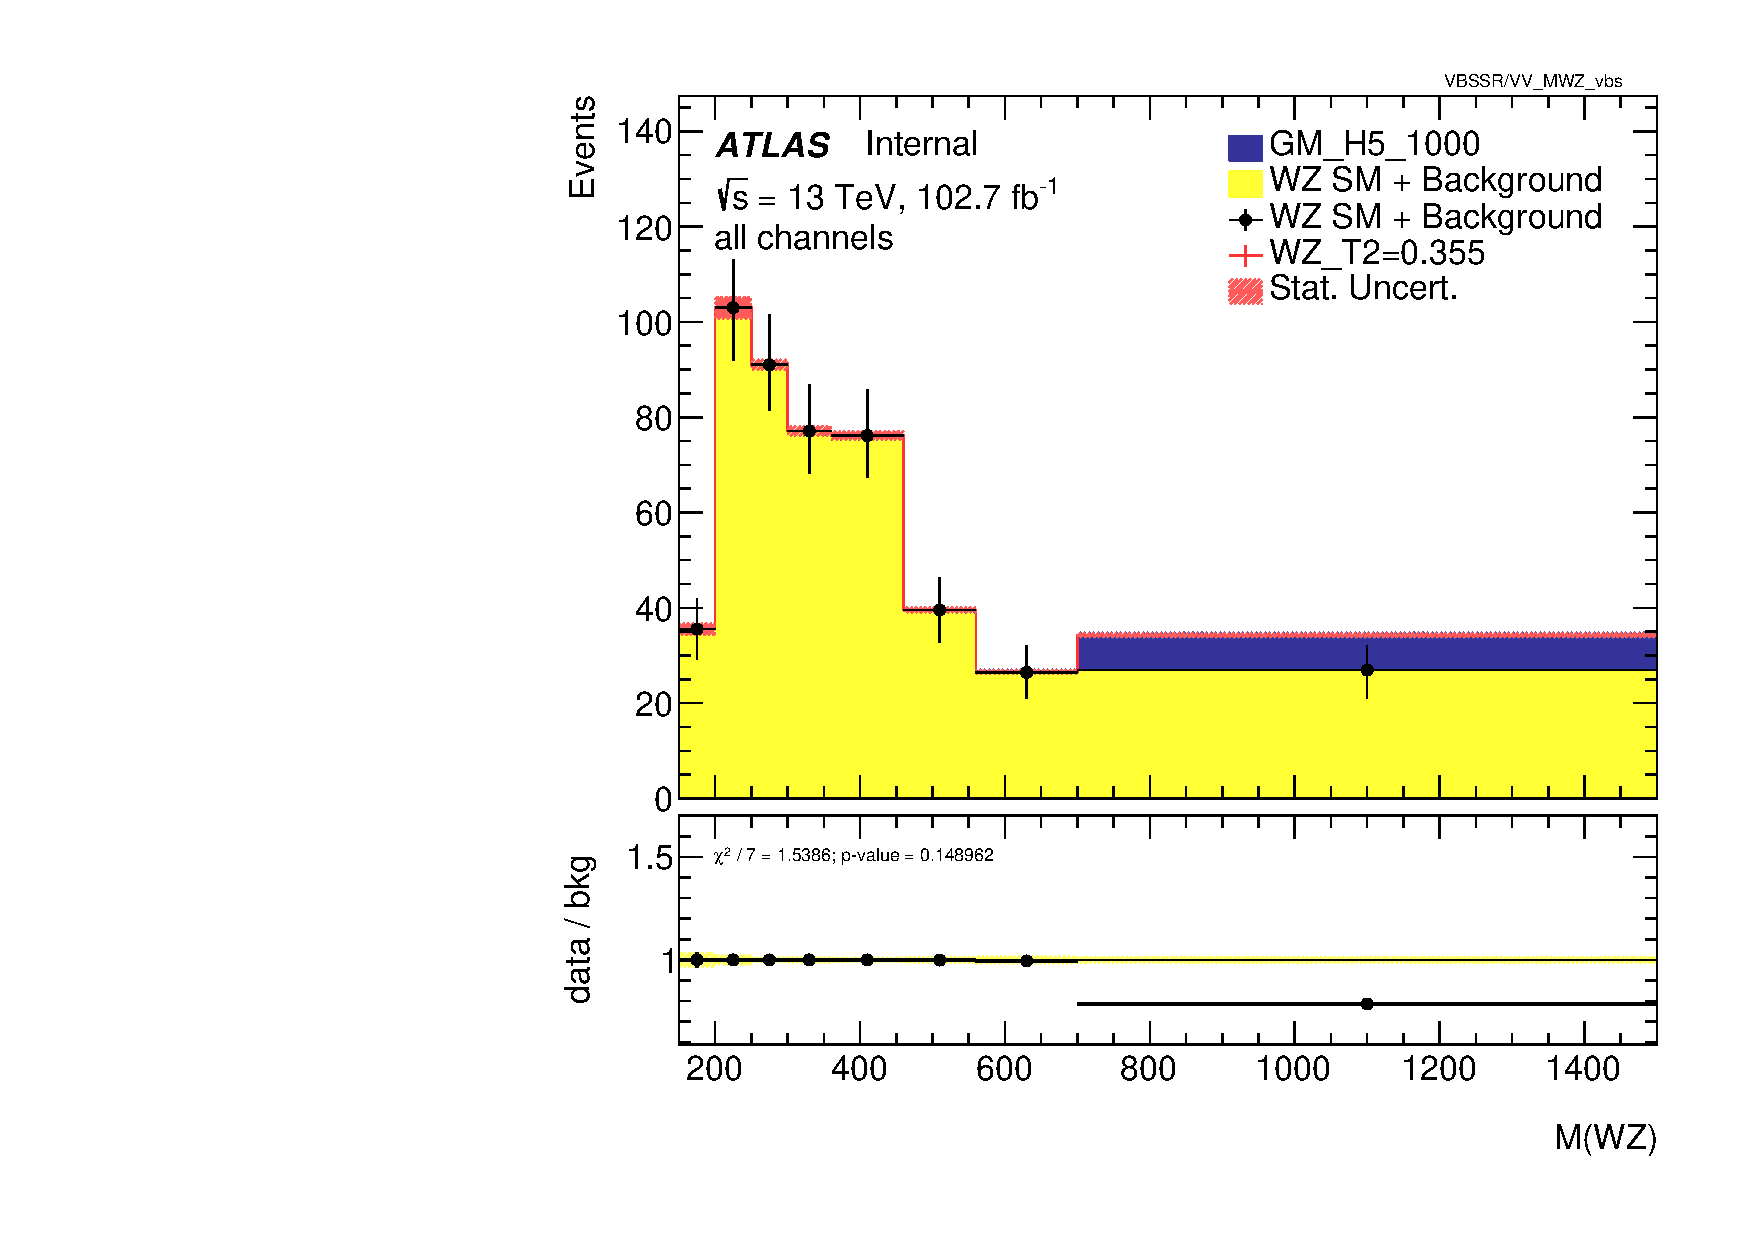
\includegraphics[width=\textwidth]{Plots/ALL_MWZ_right_color/GM_H5_1000/T2/2022-05-07/VBSSR/all_VV_MWZ_vbs.pdf}
    \end{subfigure}

    \caption{Invariant mass for parameters S1, M0, M1, T0, T1, T2 with best fit value for 1000 GeV resonance}
    \label{fig:all_mwz_1000}
\end{figure}

\begin{figure}[h]

    \centering
    \begin{subfigure}{0.45\textwidth}
        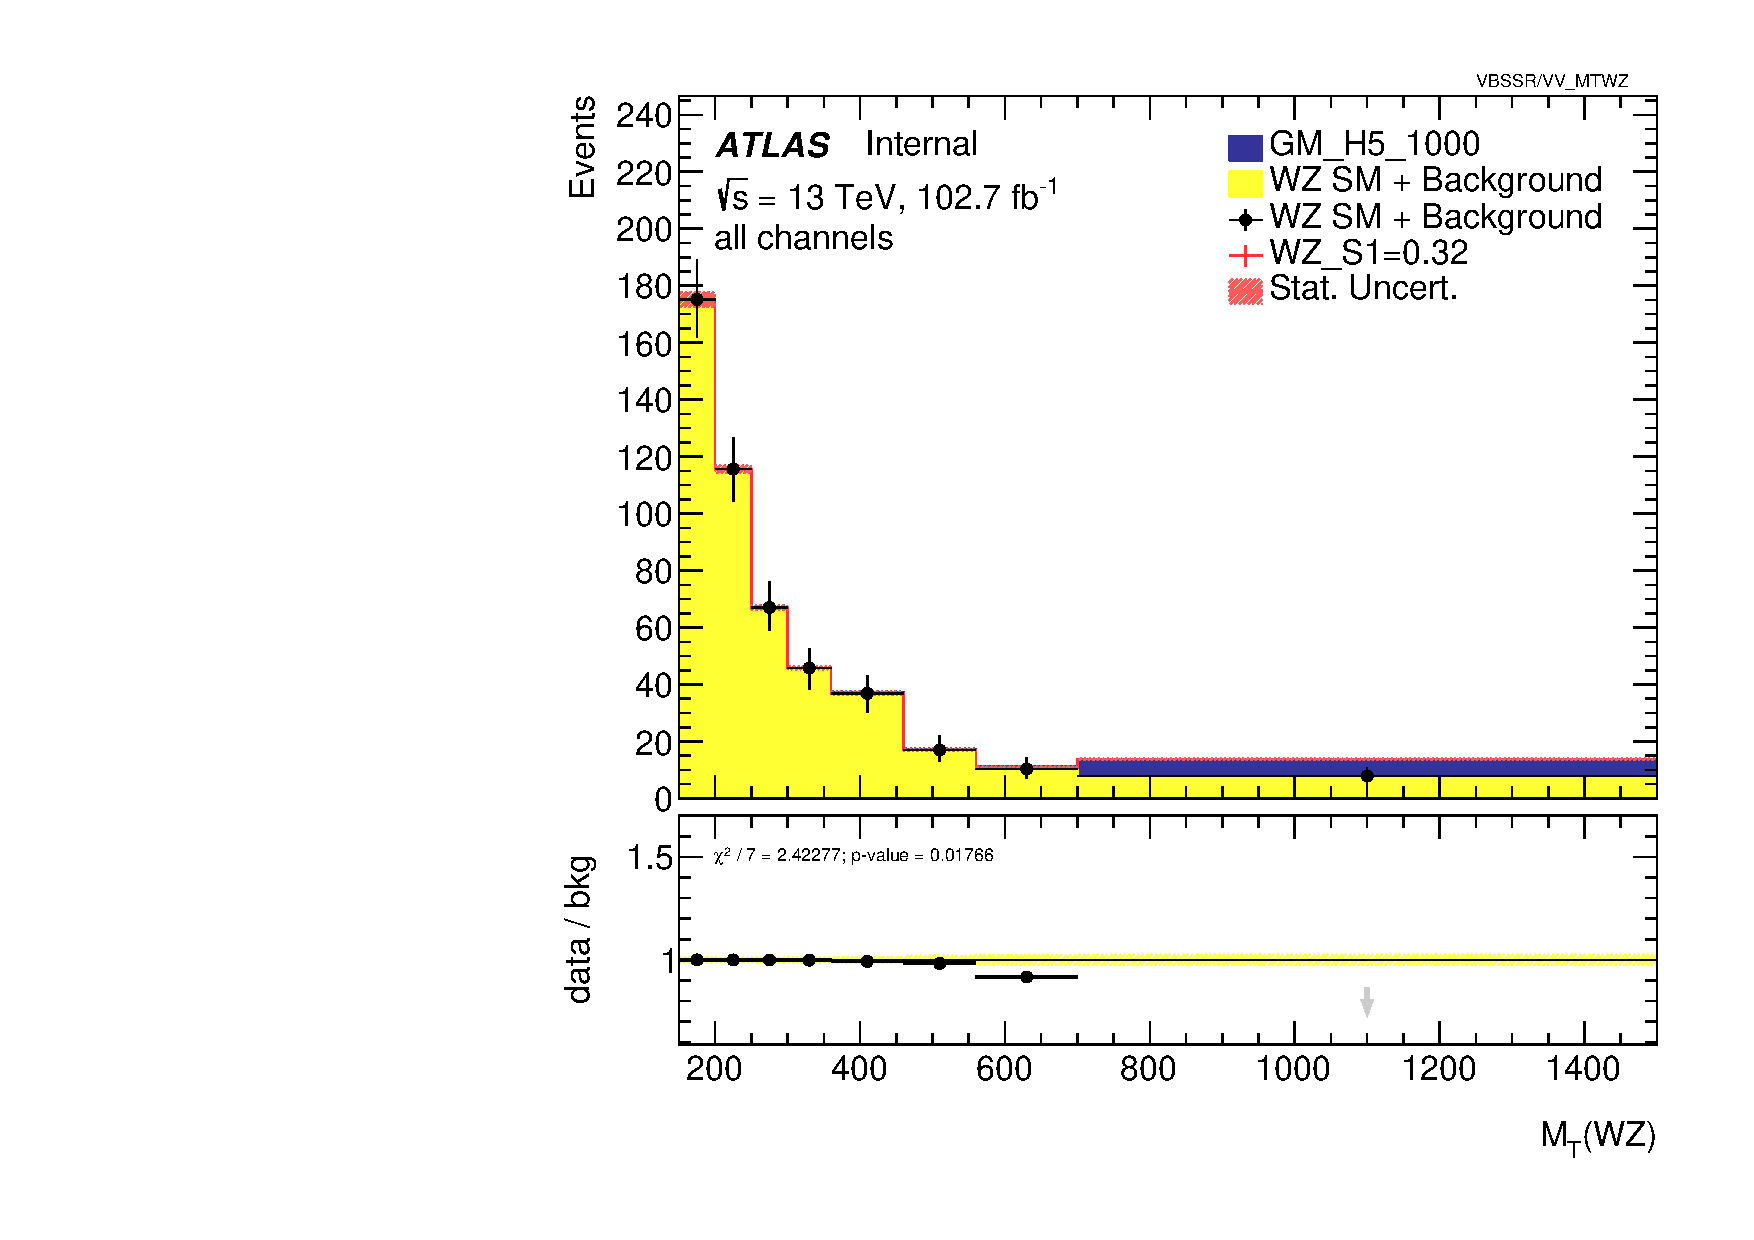
\includegraphics[width=\textwidth]{Plots/ALL_MTWZ_right_color/GM_H5_1000/S1/2022-05-07/VBSSR/all_VV_MTWZ.pdf}
    \end{subfigure}
    \begin{subfigure}{0.45\textwidth}
        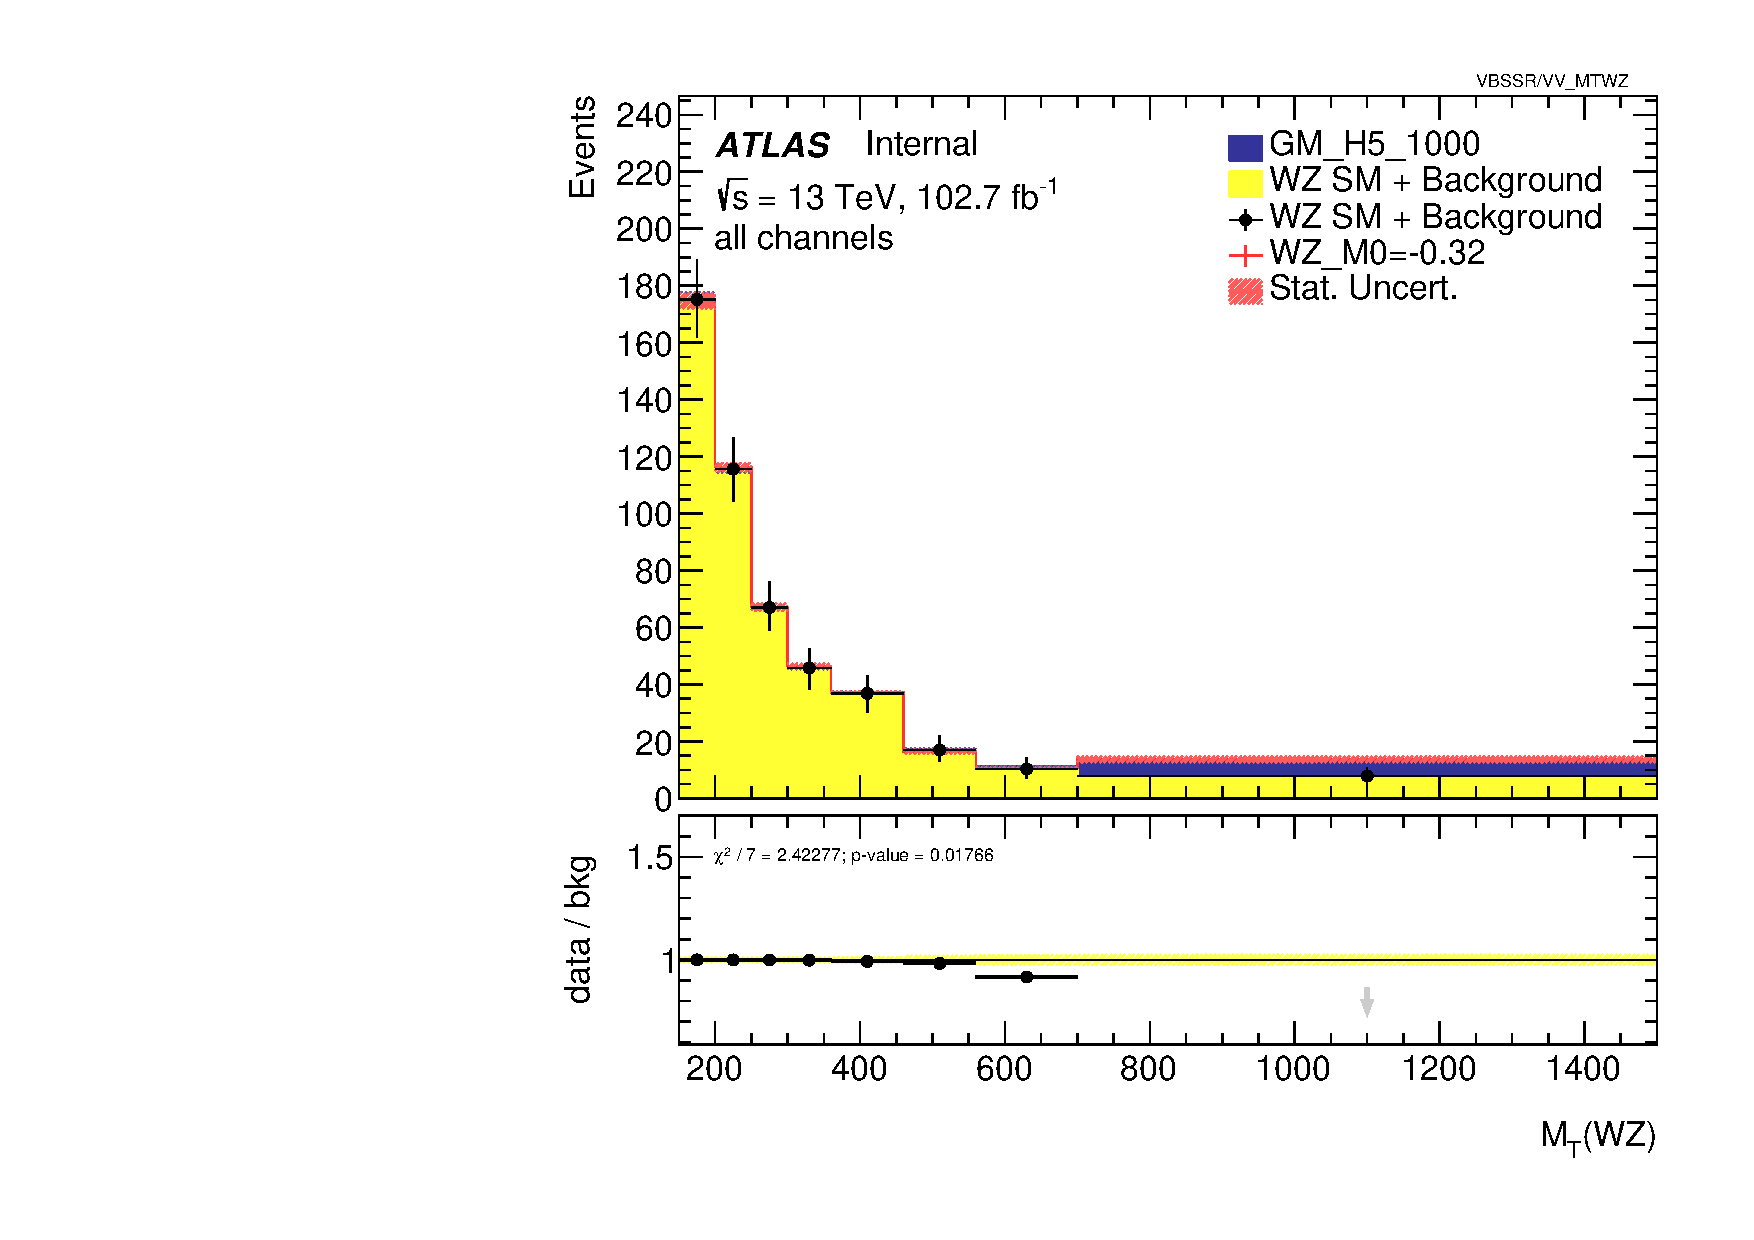
\includegraphics[width=\textwidth]{Plots/ALL_MTWZ_right_color/GM_H5_1000/M0/2022-05-07/VBSSR/all_VV_MTWZ.pdf}
    \end{subfigure}
    \begin{subfigure}{0.45\textwidth}
        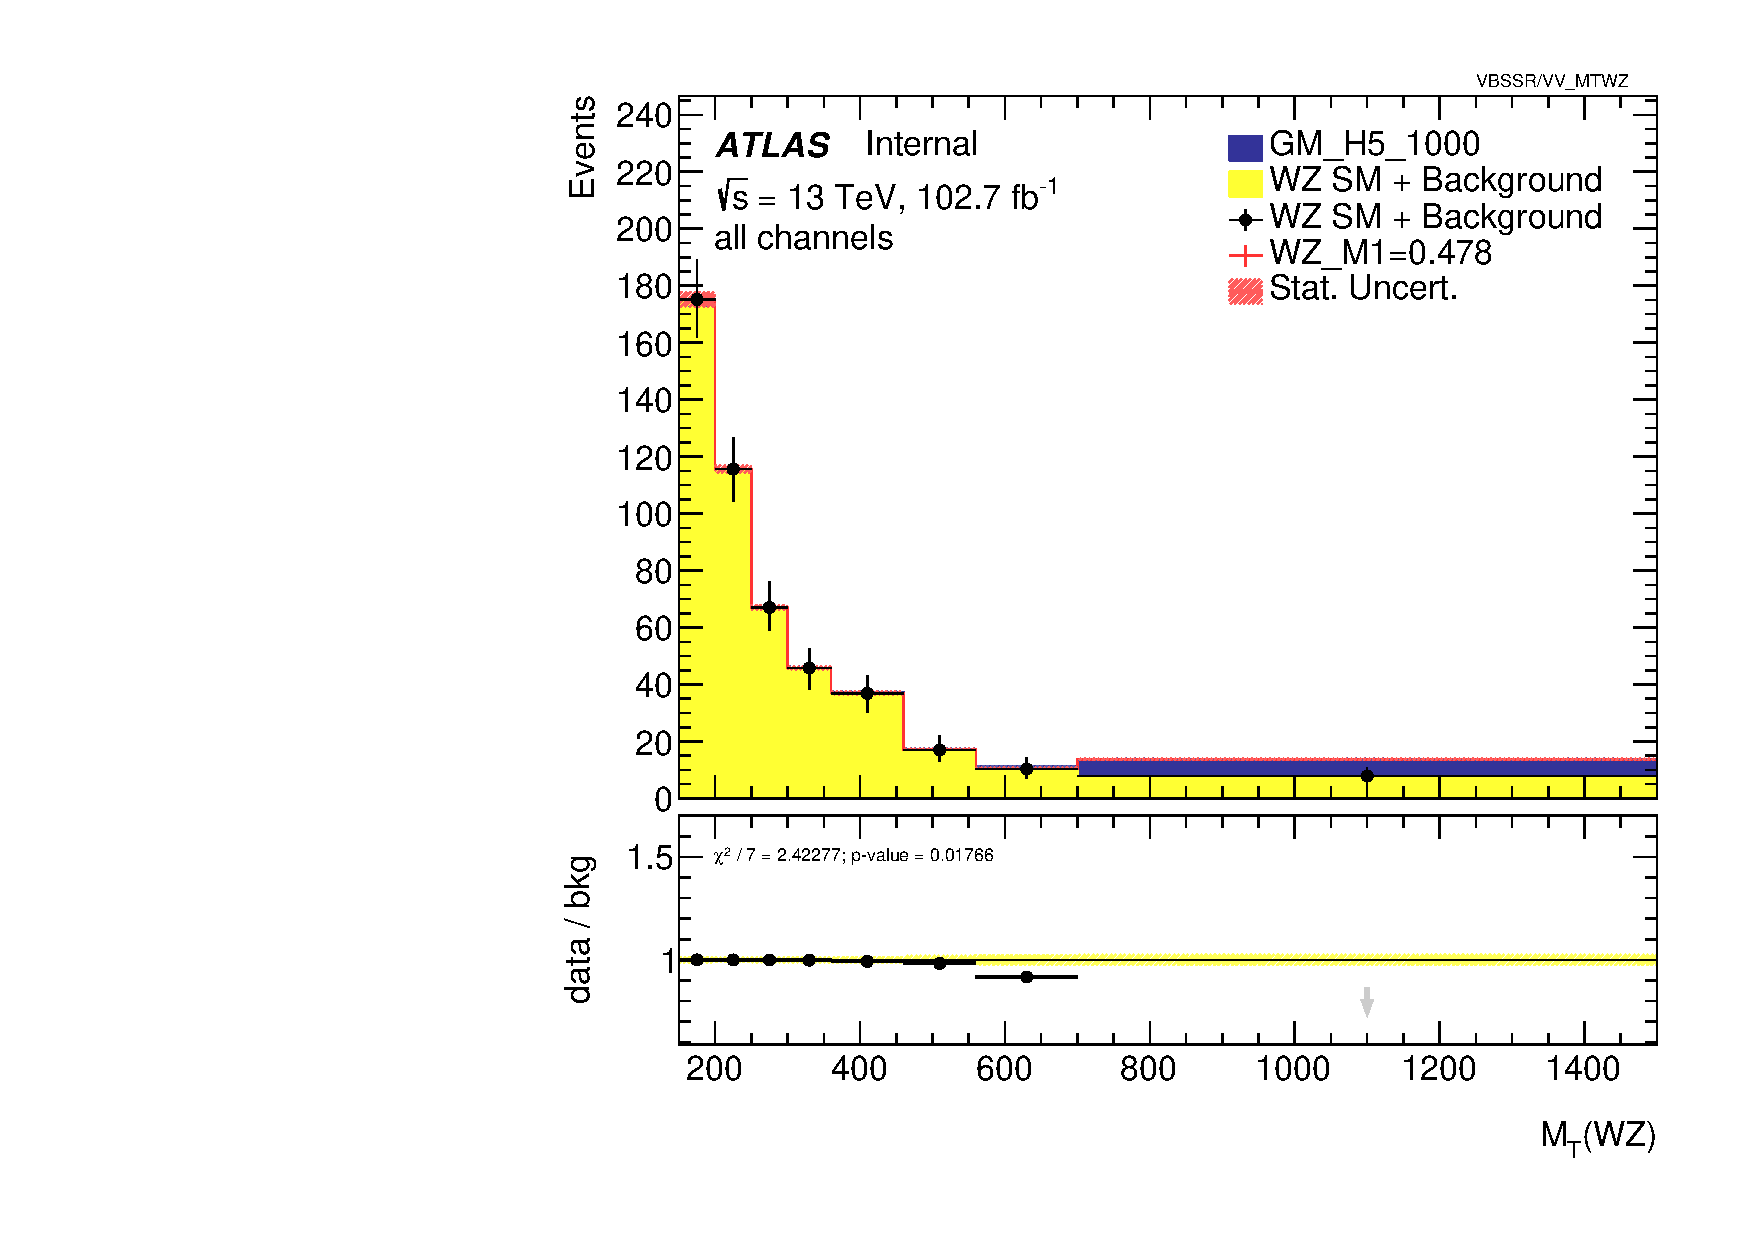
\includegraphics[width=\textwidth]{Plots/ALL_MTWZ_right_color/GM_H5_1000/M1/2022-05-07/VBSSR/all_VV_MTWZ.pdf}
    \end{subfigure}
    \begin{subfigure}{0.45\textwidth}
        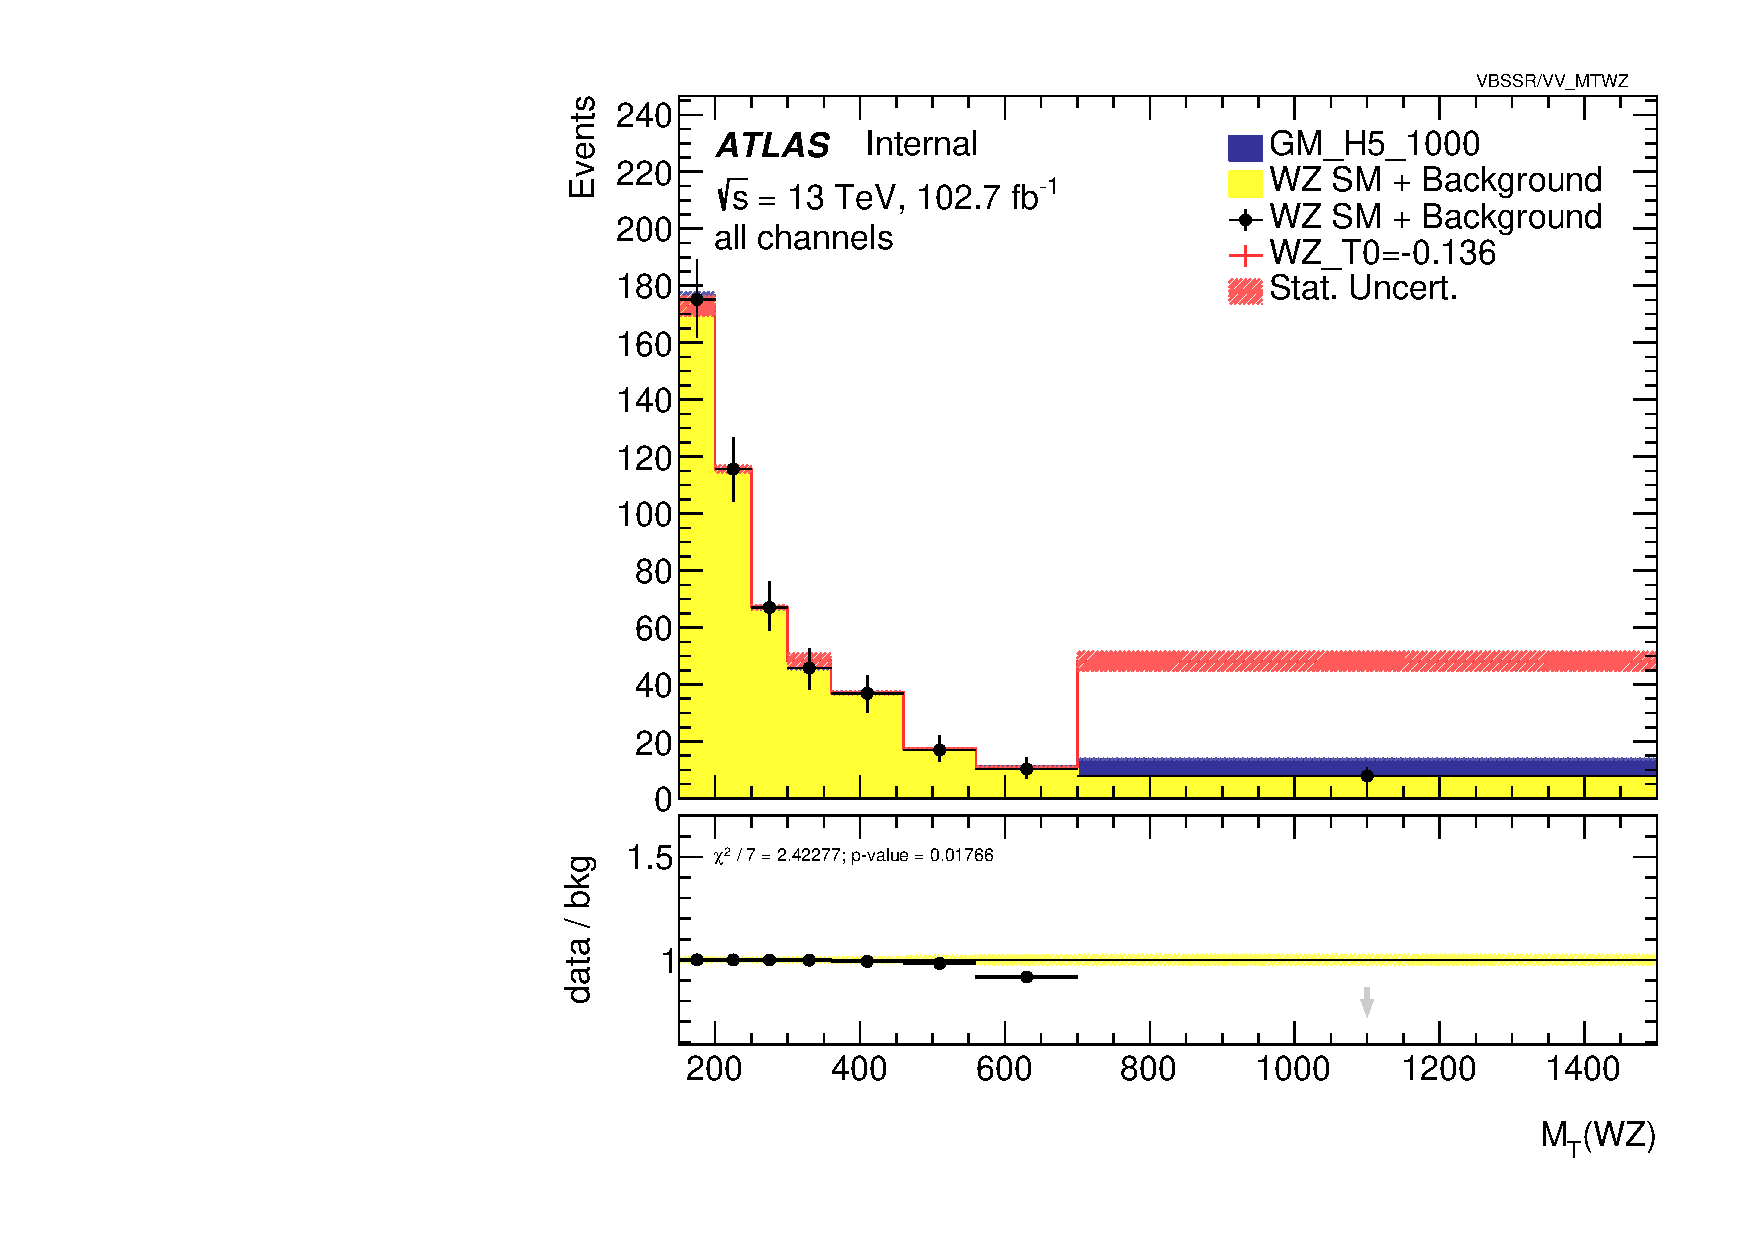
\includegraphics[width=\textwidth]{Plots/ALL_MTWZ_right_color/GM_H5_1000/T0/2022-05-07/VBSSR/all_VV_MTWZ.pdf}
    \end{subfigure}
    \begin{subfigure}{0.45\textwidth}
        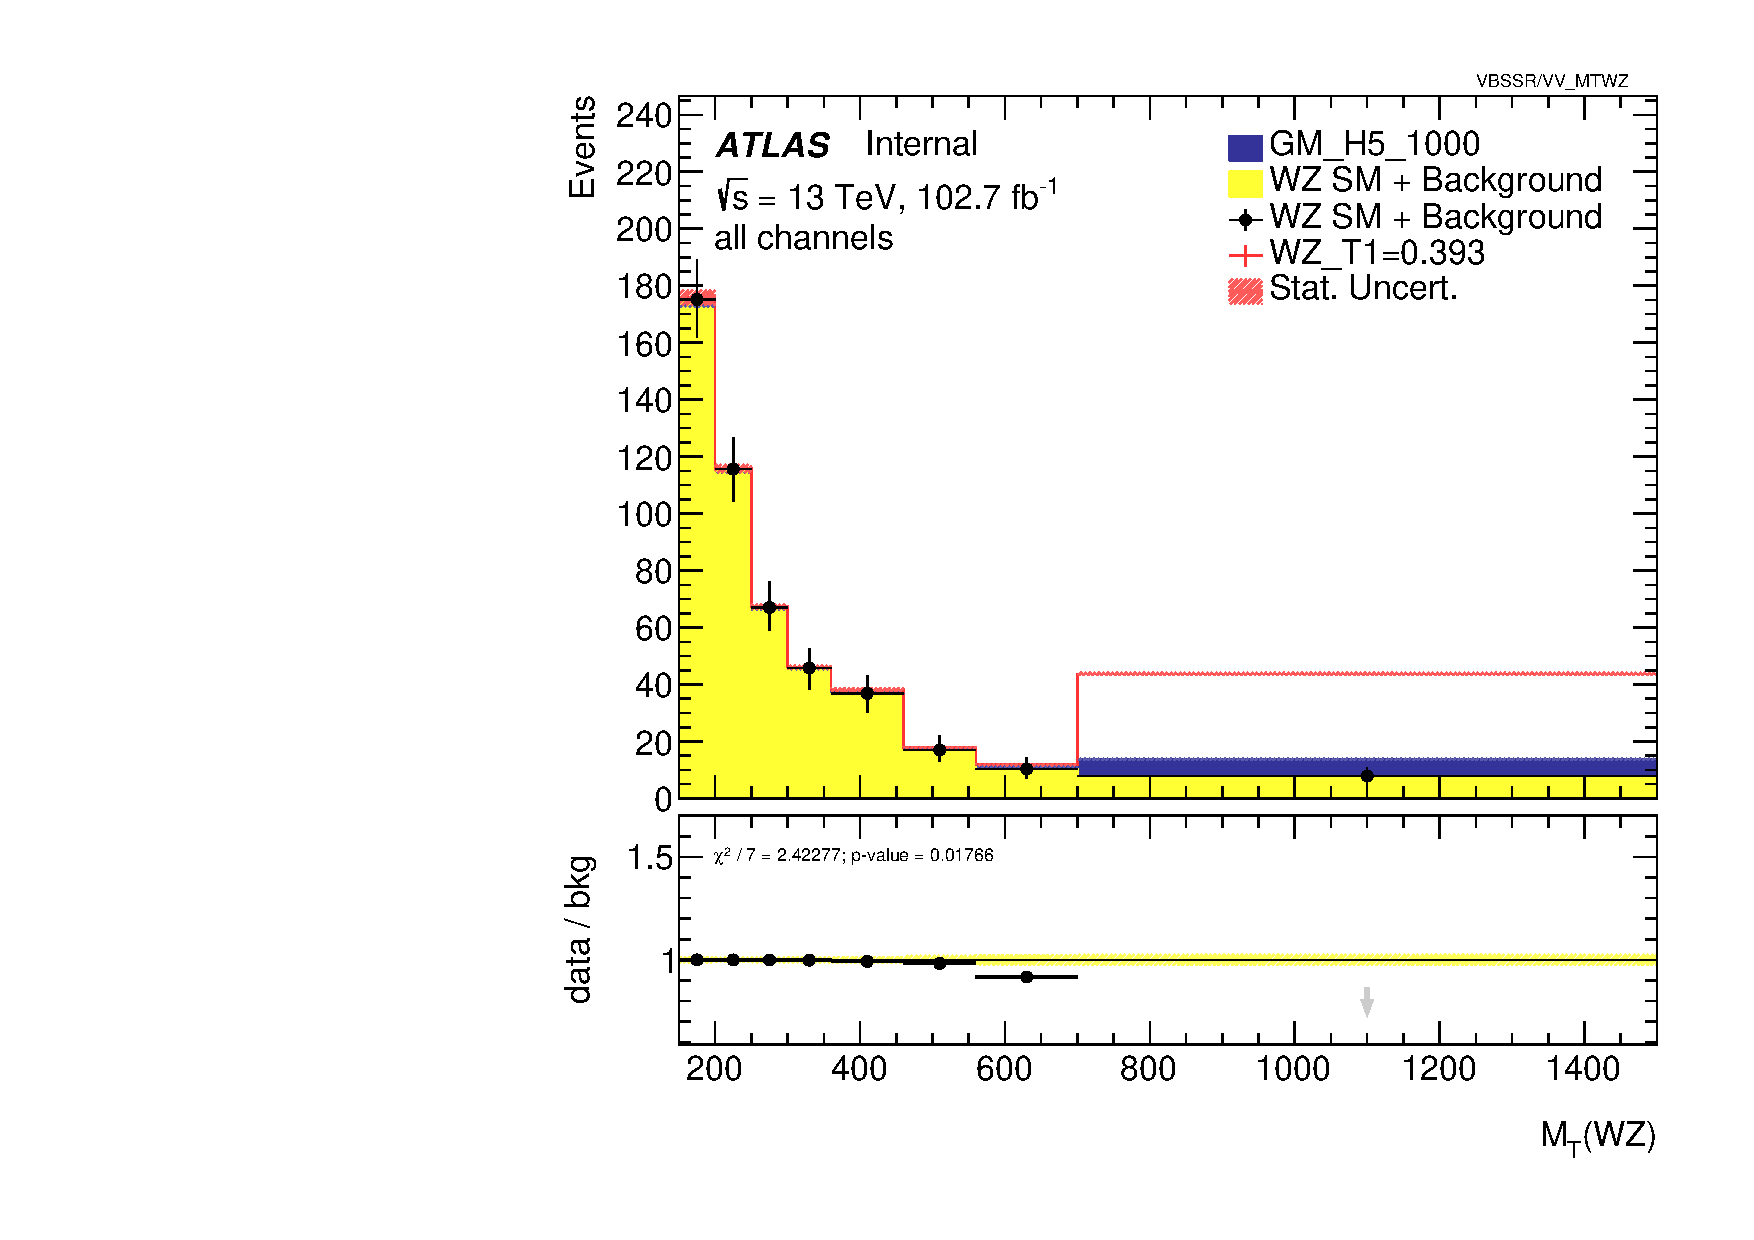
\includegraphics[width=\textwidth]{Plots/ALL_MTWZ_right_color/GM_H5_1000/T1/2022-05-07/VBSSR/all_VV_MTWZ.pdf}
    \end{subfigure}
    \begin{subfigure}{0.45\textwidth}
        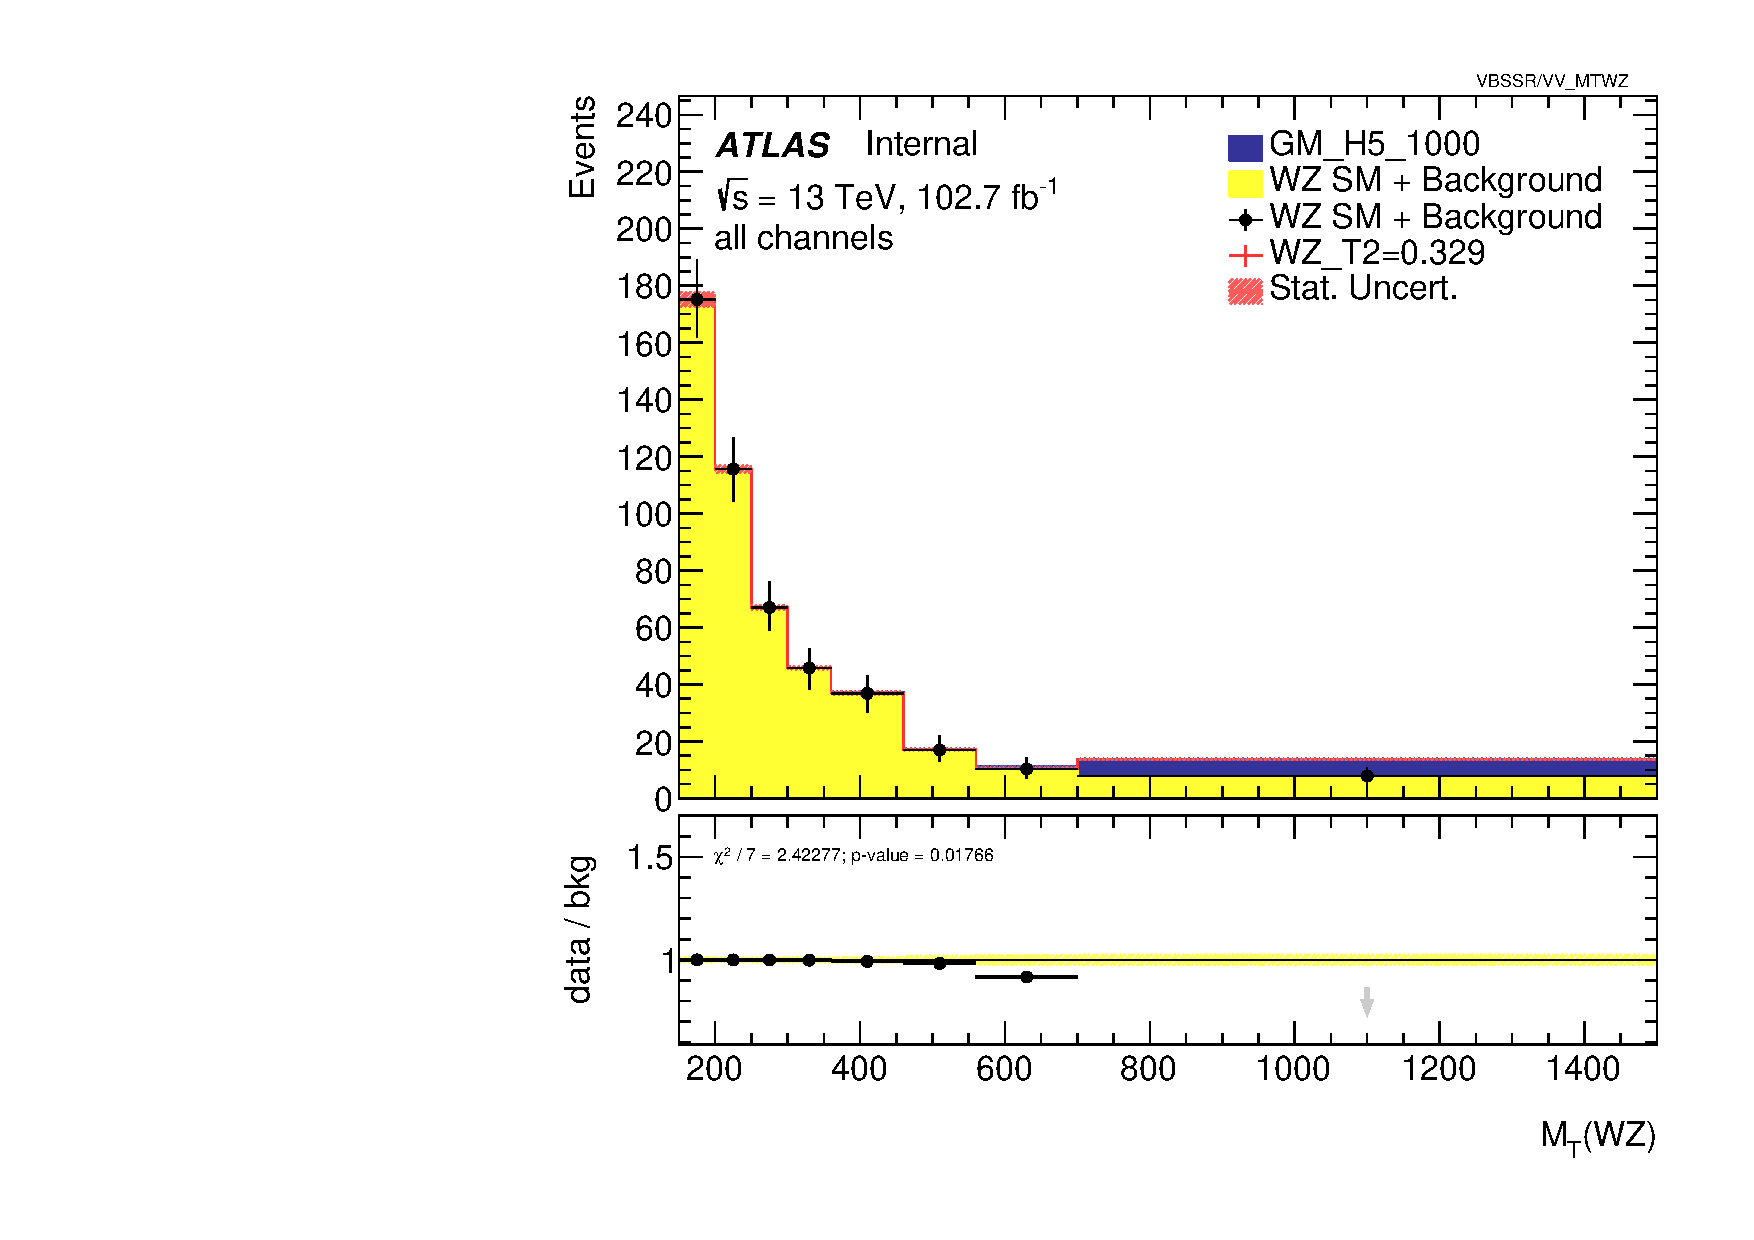
\includegraphics[width=\textwidth]{Plots/ALL_MTWZ_right_color/GM_H5_1000/T2/2022-05-07/VBSSR/all_VV_MTWZ.pdf}
    \end{subfigure}

    \caption{transverse mass for parameters S1, M0, M1, T0, T1, T2 with best fit value for 1000 GeV resonance}
    \label{fig:all_mtwz_1000}
\end{figure}




\end{document}